%% Supplementary appendices.
\chapter{平台轨迹语义压缩方法}
\label{app:platform-trajectory-compression}

原始日志逐步记录平台位置与策略，直接输入会随决策间隔和平台数量增长，且难以表达机动或驻留状态。因此，系统提取当前周期样本，经滑动窗口判定、相邻样本合并和事件汇总，生成移动与区域驻留两类语义轨迹段。

设相邻两次上层决策时刻为$t_{k-1}^{\mathrm H}$和$t_k^{\mathrm H}$。将平台$i$截至$t_k^{\mathrm H}$的原始日志按采样时刻升序排列，记为
\begin{equation}
    \mathcal T_{i,k}
    =\left(
    \left(t_l,\boldsymbol p_i^{t_l},\omega_i^{t_l}\right)
    \right)_{l=1}^{L_{i,k}},
    \qquad
    t_1<t_2<\cdots<t_{L_{i,k}}\leq t_k^{\mathrm H},
    \label{eq:appendix-trajectory-samples}
\end{equation}
其中，$L_{i,k}$为样本数，$t_l$、$\boldsymbol p_i^{t_l}$和$\omega_i^{t_l}$分别为时刻、位置和任务标签。本周期仅输出$t_l\in(t_{k-1}^{\mathrm H},t_k^{\mathrm H}]$的样本；长度不超过$W_{\mathrm{win}}$的判定窗口可调用此前最近样本，但这些历史样本不进入输出。

以第$l$个样本结尾，取$n_{i,l}=\min(W_{\mathrm{win}},l)$个样本并划分为前、后半窗$\mathcal W_{i,l}^{\mathrm{old}}$与$\mathcal W_{i,l}^{\mathrm{new}}$，其大小分别为$\lfloor n_{i,l}/2\rfloor$和$n_{i,l}-\lfloor n_{i,l}/2\rfloor$；不足两个样本时保持上一状态。两半窗中心为
\begin{equation}
    \bar{\boldsymbol p}_{i,l}^{q}
    =\frac{1}{|\mathcal W_{i,l}^{q}|}
    \sum_{h\in\mathcal W_{i,l}^{q}}\boldsymbol p_i^{t_h},
    \qquad q\in\{\mathrm{old},\mathrm{new}\}.
    \label{eq:appendix-window-centers}
\end{equation}
以前后半窗中心的欧氏距离衡量窗口内活动中心的平移量：
\begin{equation}
    d_{i,l}=\left\|
    \bar{\boldsymbol p}_{i,l}^{\mathrm{new}}
    -\bar{\boldsymbol p}_{i,l}^{\mathrm{old}}
    \right\|_2.
    \label{eq:appendix-center-shift}
\end{equation}
$d_{i,l}$衡量活动中心迁移而非瞬时速度，因此围绕固定区域盘旋也可判为驻留。

为避免$d_{i,l}$在单一阈值附近波动造成运动状态频繁切换，设置驻留进入阈值$\delta_i^{\mathrm{in}}$和驻留离开阈值$\delta_i^{\mathrm{out}}$，并满足$\delta_i^{\mathrm{in}}<\delta_i^{\mathrm{out}}$。令$m_{i,l}\in\{\mathrm{stay},\mathrm{move}\}$为第$l$个样本对应的运动状态，则滞回更新规则为
\begin{equation}
    m_{i,l}=\begin{cases}
        \mathrm{move},
        &m_{i,l-1}=\mathrm{stay}\ \land\
        d_{i,l}>\delta_i^{\mathrm{out}},\\
        \mathrm{stay},
        &m_{i,l-1}=\mathrm{move}\ \land\
        d_{i,l}\leq\delta_i^{\mathrm{in}},\\
        m_{i,l-1}, &\text{其他情况}.
    \end{cases}
    \label{eq:appendix-hysteresis-classification}
\end{equation}
最早样本初始化为$\mathrm{stay}$，后续按式~\eqref{eq:appendix-hysteresis-classification}递推；艇机采用不同阈值，以适应速度和活动半径差异。

分类后，将本周期内运动状态$m_{i,l}$与任务标签$\omega_i^{t_l}$均相同的相邻样本合并。设第$s$段的连续索引集合为$\mathcal L_{i,s}$，首尾索引为
\begin{equation*}
    l_{i,s}^{\mathrm{from}}=\min\mathcal L_{i,s},
    \qquad
    l_{i,s}^{\mathrm{to}}=\max\mathcal L_{i,s}.
\end{equation*}
记起止时刻为$t_{i,s}^{\mathrm{from}}$、$t_{i,s}^{\mathrm{to}}$，位置为$\boldsymbol p_{i,s}^{\mathrm{from}}$、$\boldsymbol p_{i,s}^{\mathrm{to}}$，统一任务标签为$\omega_{i,s}$。移动段保留这些边界量与样本数：
\begin{equation}
    \mathcal S_{i,s}^{\mathrm{move}}
    =\left(t_{i,s}^{\mathrm{from}},t_{i,s}^{\mathrm{to}},
    \boldsymbol p_{i,s}^{\mathrm{from}},\boldsymbol p_{i,s}^{\mathrm{to}},
    \omega_{i,s},|\mathcal L_{i,s}|\right).
    \label{eq:appendix-moving-segment}
\end{equation}
对于驻留段，以段内平均位置和活动半径代替全部位置点：
\begin{equation}
    \begin{aligned}
    \bar{\boldsymbol p}_{i,s}
    &=\frac{1}{|\mathcal L_{i,s}|}
      \sum_{l\in\mathcal L_{i,s}}\boldsymbol p_i^{t_l},\\
    \rho_{i,s}
    &=\max_{l\in\mathcal L_{i,s}}
      \left\|\boldsymbol p_i^{t_l}-\bar{\boldsymbol p}_{i,s}\right\|_2,\\
    \mathcal S_{i,s}^{\mathrm{stay}}
    &=\left(t_{i,s}^{\mathrm{from}},t_{i,s}^{\mathrm{to}},
      \bar{\boldsymbol p}_{i,s},\rho_{i,s},
      \omega_{i,s},|\mathcal L_{i,s}|\right).
    \end{aligned}
    \label{eq:appendix-stay-segment}
\end{equation}
其中，$\rho_{i,s}$为驻留活动半径；任务标签变化时即使运动状态不变也切分轨迹段。图~\ref{fig:appendix-trajectory-compression}给出压缩示例。

\begin{figure}[!htbp]
    \centering
    \includegraphics[width=0.96\textwidth]{\detokenize{轨迹压缩.png}}
    \caption{平台原始轨迹的语义压缩示意图}
    \label{fig:appendix-trajectory-compression}
\end{figure}

系统同时提取区间$(t_{k-1}^{\mathrm H},t_k^{\mathrm H}]$内的发射、发现、毁伤和失效事件及其时刻、平台与目标关系。最终输出包含$t_k^{\mathrm H}$的状态快照、语义轨迹段和增量事件，避免重复位置占用上下文。

\chapter{上层指挥决策器提示词模板}
\label{app:llm-prompt-templates}

本附录列出五类大模型节点的提示词。$\langle \dot \rangle$由第$k$次上层决策的状态填充，集合、平台状态和事件均序列化为结构化文本；$\boldsymbol\zeta_{j,k}$表示第$j$个威胁中心。

\section{威胁位置推断提示词}

该模板用于已观测展开集群成员但核心位置未知的情况。

\begin{quote}\small
\textbf{系统指令：}你是敌方集群核心位置推断专家。无人艇承担核心和主要火力载荷，无人机围绕其协同。仅依据已观测成员位置、类型、集群状态和编组知识推断核心；不得虚构平台或将初始情报当作当前位置。只输出结构化对象。

\textbf{动态输入：}当前待推断威胁中心编号为$\langle j\rangle$，集群状态为$\langle\text{集群状态}\rangle$；已观测成员为$\langle\mathcal M_{j,k}^{\mathrm{obs}}\rangle$，每个成员包含平台编号、平台类型和当前位置；已知敌方编组规律为$\langle\text{敌方艇机编组知识}\rangle$。请估计集群核心位置。

\textbf{输出格式：}\{``position'':[$x$,$y$]\}。
\end{quote}

输出缺少有效二维坐标或调用失败时，程序以已观测成员的几何中心作为$\widehat{\boldsymbol p}_{j,k}^{\mathrm{core}}$。

\section{态势总结提示词}

该模板从结构化上层状态中识别需调整任务分配的情况。

\begin{quote}\small
\textbf{系统指令：}你是战场态势分析专家。你只能依据输入事实和给定知识进行判断，不得虚构距离、平台身份、因果关系或持续时间；证据不足时必须写“证据不足”，不得将可能性表述为已经发生的事实。

平台状态、压缩轨迹、事件、分组、威胁中心、当前数量和程序信号均为权威事实。威胁中心是推断记录而非环境真值，置信度达阈值仅表示可用于规划；紧急防守信号为真时必须增加阵位防守力量。

请逐项判断以下五种情况：

1. 未探明威胁数量大于当前执行覆盖搜索任务的无人机数量，是否需要增加侦察力量；

2. 是否出现新探明且尚未展开的威胁，并且需要增加主动拦截力量；

3. 敌方是否进入友方外沿且保护中心内侧防守力量不足；

4. 原主动拦截编组是否已完成攻击任务，需要转入防守或其他拦截任务；

5. 存活侦察平台是否完成了某一威胁的确认任务，可以减少覆盖搜索力量；

状态仅可为“成立”“不成立”或“证据不足”；成立时给出对应措施。依据须可追溯至输入，不得增设判断标准。只输出结构化对象。

\textbf{动态输入：}战场知识为$\langle\text{战场背景与敌方编组知识}\rangle$；任务知识为$\langle\text{三类任务定义}\rangle$；情况判据为$\langle\text{任务调整判据}\rangle$；结构化事实为$\langle\boldsymbol s_k^{\mathrm H}\rangle$。

\textbf{输出格式：}
\{``judgments'':[\{``situation'':编号，``status'':``成立$|$不成立$|$证据不足''，``judgment'':``情况判断''，``evidence'':[``直接事实依据'']\}]，``solutions'':[\{``situation'':编号，``measure'':``对应措施''\}]\}。
\end{quote}

核查未通过时追加上一版草案与核查问题，要求仅作最小修正，不引入新判断。

\section{事实核查提示词}

该节点仅核查事实，不重新决策。

\begin{quote}\small
\textbf{系统指令：}你是有限权限的事实核查员，仅识别会改变成立状态或措施的硬错误，不进行战术规划。

仅报告两类问题：草案中的平台编号、数量、状态、事件或位置与原始事实矛盾；成立状态或措施违反显式判据。每项须给出事实位置、决策影响和最小修正。

不得新增占用关系、部署或拦截要求、阈值和评价维度，也不得因措辞、其他解释或保守偏好判定失败。若无影响决策的问题，判定通过且问题列表为空；只输出核查结果。

\textbf{动态输入：}事实字段定义为$\langle\text{字段语义}\rangle$；任务调整判据为$\langle\text{显式判据}\rangle$；原始结构化事实为$\langle\boldsymbol s_k^{\mathrm H}\rangle$；待核查的态势总结草案为$\langle\text{总结草案}\rangle$。

\textbf{输出格式：}
\{``passed'':真或假，``issues'':[\{``situation'':编号，``type'':``事实矛盾或规则违反''，``fact\_paths'':[``原始事实位置'']，``decision\_impact'':真或假，``problem'':``问题说明''，``required\_revision'':``最小修正''\}]\}。
\end{quote}

核查未通过时仅允许总结节点修正一次；输出无法解析则保留原草案并记录异常。

\section{结论封装提示词}

该节点将已核查内容压缩为资源规划所需信息，不新增判断。

\begin{quote}\small
\textbf{系统指令：}你是态势结论编辑。保留资源规划所需的成立情况、关键数量、威胁中心编号、依据和措施，删除重复及无关推理；不得新增事实。证据不足时保守表述，不得把推测写成事实；仅保留成立情况对应的措施，无情况成立则保持当前分配。只输出结构化对象。

\textbf{动态输入：}修正后的态势总结为$\langle\text{总结草案}\rangle$；最新事实核查结果为$\langle\text{核查结果}\rangle$。

\textbf{输出格式：}\{``condition'':``精简后的情况''，``evidence'':``支持判断的关键事实''，``solution'':``对应措施''\}。
\end{quote}

\section{资源规划提示词}

该节点只确定三类任务的资源数量与拦截对象，不绑定平台编号。

\begin{quote}\small
\textbf{系统指令：}你是无人集群资源规划专家。依据上一节点的情况、依据和措施，调整三类任务的平台数量并选择主动拦截中心。

必须遵守以下约束：三类任务的平台数量均为非负整数，且数量之和等于当前可用平台总数；覆盖搜索任务只能使用无人机，其数量不得超过可用无人机数量；主动拦截数量大于零时，必须存在可处置的高置信度威胁中心，并满足给定的无人艇—无人机编成比例；无可处置威胁时，主动拦截数量必须为零；紧急防守信号为真时，优先增加阵位防守数量；拦截对象只能从输入给出的候选威胁中心中选择。

结构化数量、候选中心和安全信号为权威事实，与自然语言结论冲突时以前者为准。不得指定平台编号；调整摘要用一句话说明变化方向。只输出结构化对象。

\textbf{动态输入：}上一节点结论为$\langle\text{情况、依据与措施}\rangle$；可用平台数量为$\langle N_k^{\mathrm U},N_k^{\mathrm S}\rangle$；当前任务数量为$\langle\text{三类任务当前数量}\rangle$；威胁态势为$\langle\mathcal C_k\rangle$；候选拦截对象为$\langle\text{达到置信度阈值且仍有效的威胁中心}\rangle$；任务触发原因和安全约束为$\langle\text{触发信号与编成约束}\rangle$。

\textbf{输出格式：}
\{``task\_counts'':\{``recon'':整数，``attack'':整数，``defend'':整数\}，``attack\_targets'':[威胁中心编号]，``adjustment'':``任务数量调整摘要''\}。
\end{quote}

程序校验数量守恒、平台资格、目标有效性和艇机比例。首次失败时追加原结果与违反约束，要求保持战术意图并仅修正违规项；再次失败则启用确定性规则。

\section{任务绑定节点规则}
\label{app:task-binding-rules}

任务绑定节点将资源数量和主动拦截对象确定性转换为平台级联合动作。设可用平台及无人机集合分别为$\mathcal N_k$和$\mathcal N_k^{\mathrm U}$，资源规划结果为
\begin{equation}
    \boldsymbol n_k^{\mathrm{task}}
    =\left(n_k^{\mathrm{rec}},n_k^{\mathrm{atk}},n_k^{\mathrm{def}}\right),
    \qquad
    n_k^{\mathrm{rec}}+n_k^{\mathrm{atk}}+n_k^{\mathrm{def}}
    =|\mathcal N_k|,
    \label{eq:appendix-binding-task-counts}
\end{equation}
以$\mathcal C_k^{\mathrm{atk}}\subseteq\mathcal C_k$表示拦截对象。平台选择优先保持上一周期策略，再按到相关威胁中心的距离和编号排序。定义
\begin{equation}
    \delta_{i,k}^{q}=\begin{cases}
        0,&\omega_{i,k-1}=\omega^q,\\
        1,&\omega_{i,k-1}\neq\omega^q,
    \end{cases}
    \qquad q\in\{\mathrm{rec},\mathrm{atk}\},
    \label{eq:appendix-binding-continuity}
\end{equation}
$d_{i,k}^{\mathrm{rec}}$和$d_{i,k}^{\mathrm{atk}}$分别为平台$i$到最近低置信度中心和指定拦截中心的距离。按$(\delta_{i,k}^{q},d_{i,k}^{q},i)$升序排列，可依次保证策略连续性、距离和编号优先级。

主动拦截编组中无人机和无人艇的数量分别记为$n_k^{\mathrm{A,U}}$和$n_k^{\mathrm{A,S}}$。在资源允许时，编组满足
\begin{equation}
    n_k^{\mathrm{A,U}}+n_k^{\mathrm{A,S}}=n_k^{\mathrm{atk}},
    \qquad
    2n_k^{\mathrm{A,S}}\leq n_k^{\mathrm{A,U}}
    \leq3n_k^{\mathrm{A,S}},
    \label{eq:appendix-binding-attack-ratio}
\end{equation}
即每艘火力核心无人艇配置$2$至$3$架无人机，优先接近$2{:}1$；资源不足以合法编组时直接采用安全兜底。完整过程见算法~\ref{alg:upper-task-binding}。

\begin{algorithm}[!htbp]
\caption{上层任务绑定与安全校验}
\label{alg:upper-task-binding}
\small
\begin{algorithmic}[1]
\Require 可用平台$\mathcal N_k$及其类型、位置和上一周期任务；任务数量$\boldsymbol n_k^{\mathrm{task}}$；主动拦截对象$\mathcal C_k^{\mathrm{atk}}$；威胁中心集合$\mathcal C_k$
\Ensure 平台级联合任务$\boldsymbol\omega_k$及三类任务平台集合$\mathcal I_{\mathrm{rec},k}$、$\mathcal I_{\mathrm{atk},k}$和$\mathcal I_{\mathrm{def},k}$
\State 初始化三个任务平台集合为空集
\If{任务数量不满足式~\eqref{eq:appendix-binding-task-counts}，或$n_k^{\mathrm{rec}}>|\mathcal N_k^{\mathrm U}|$}
    \State 将全部平台分配至$\mathcal I_{\mathrm{def},k}$，并返回安全防守任务
\EndIf
\If{$n_k^{\mathrm{atk}}>0$且$\mathcal C_k^{\mathrm{atk}}$为空，或集合中存在无效威胁中心}
    \State 将全部平台分配至$\mathcal I_{\mathrm{def},k}$，并返回安全防守任务
\EndIf
\State 按$(\delta_{i,k}^{\mathrm{rec}},d_{i,k}^{\mathrm{rec}},i)$升序排列$\mathcal N_k^{\mathrm U}$
\State 取前$n_k^{\mathrm{rec}}$个平台构成$\mathcal I_{\mathrm{rec},k}$
\State $\mathcal N_k^{\mathrm{rem}}\gets\mathcal N_k\setminus\mathcal I_{\mathrm{rec},k}$
\State 枚举满足式~\eqref{eq:appendix-binding-attack-ratio}且不超过$\mathcal N_k^{\mathrm{rem}}$艇机资源的可行编成集合$\mathcal F_k$
\If{$n_k^{\mathrm{atk}}>0$且$\mathcal F_k=\varnothing$}
    \State 将全部平台分配至$\mathcal I_{\mathrm{def},k}$，并返回安全防守任务
\EndIf
\If{$n_k^{\mathrm{atk}}>0$}
    \State 从$\mathcal F_k$中选取最接近$2{:}1$且保留较多无人艇火力核心的编成$(n_k^{\mathrm{A,U}},n_k^{\mathrm{A,S}})$
    \State 分别按$(\delta_{i,k}^{\mathrm{atk}},d_{i,k}^{\mathrm{atk}},i)$升序排列剩余无人机与无人艇
    \State 选择前$n_k^{\mathrm{A,U}}$架无人机和前$n_k^{\mathrm{A,S}}$艘无人艇构成$\mathcal I_{\mathrm{atk},k}$
\EndIf
\State $\mathcal I_{\mathrm{def},k}\gets\mathcal N_k\setminus(\mathcal I_{\mathrm{rec},k}\cup\mathcal I_{\mathrm{atk},k})$
\State 根据三个平台集合生成$\boldsymbol\omega_k$，并附加主动拦截对象$\mathcal C_k^{\mathrm{atk}}$
\State 检查平台可用性、分配唯一性、分配完备性、任务数量、平台资格、目标有效性和艇机编成
\If{任一检查未通过}
    \State $\mathcal I_{\mathrm{rec},k},\mathcal I_{\mathrm{atk},k}\gets\varnothing$，$\mathcal I_{\mathrm{def},k}\gets\mathcal N_k$
    \State 生成全员阵位防守的安全任务$\boldsymbol\omega_k$
\EndIf
\State \Return $\boldsymbol\omega_k$，$\mathcal I_{\mathrm{rec},k}$，$\mathcal I_{\mathrm{atk},k}$，$\mathcal I_{\mathrm{def},k}$
\end{algorithmic}
\end{algorithm}

该顺序保证覆盖搜索资格和主动拦截编成约束；三个集合须两两不交、并集为$\mathcal N_k$且规模符合规划，否则执行全员阵位防守。

\begingroup
\let\clearpage\relax
\chapter{覆盖搜索热点方向补偿方法}
\label{app:search-hotspot-compensation}
\endgroup

当无人机进入已充分搜索或低概率区域时，八个方向的新增熵减均可能接近零，局部信息增益无法提供脱离方向。热点补偿仅在此类低信息区域提供辅助引导。

对于无人机$i$的候选动作$a$，以动作后探测范围相对于当前位置探测范围新增的网格集合为$\Delta\mathcal B_i^t(a)$，对应的潜在新增信息量为
\begin{equation}
    I_i^t(a)=
    \sum_{(x_{\mathrm g},y_{\mathrm g})\in\Delta\mathcal B_i^t(a)}
    H_{x_{\mathrm g},y_{\mathrm g}}^t.
    \label{eq:rec-potential-new-information}
\end{equation}
若八个方向的$I_i^t(a)$均低于阈值，则提取概率图中的高概率网格，经连通域合并并滤除小面积区域。有效热点$\mathcal V_m^{\mathrm{hot}}$的概率加权中心为
\begin{equation}
    \boldsymbol c_m^t=
    \frac{
    \displaystyle
    \sum_{(x_{\mathrm g},y_{\mathrm g})\in\mathcal V_m^{\mathrm{hot}}}
    p_{x_{\mathrm g},y_{\mathrm g}}^t
    \boldsymbol c_{x_{\mathrm g},y_{\mathrm g}}}
    {
    \displaystyle
    \sum_{(x_{\mathrm g},y_{\mathrm g})\in\mathcal V_m^{\mathrm{hot}}}
    p_{x_{\mathrm g},y_{\mathrm g}}^t},
    \label{eq:rec-hotspot-center}
\end{equation}
选择最近的热点中心作为补偿目标$\boldsymbol c_i^{t,*}$，其几何关系见图~\ref{fig:rec-hotspot-center-angle}。

\begin{figure}[!htbp]
    \centering
    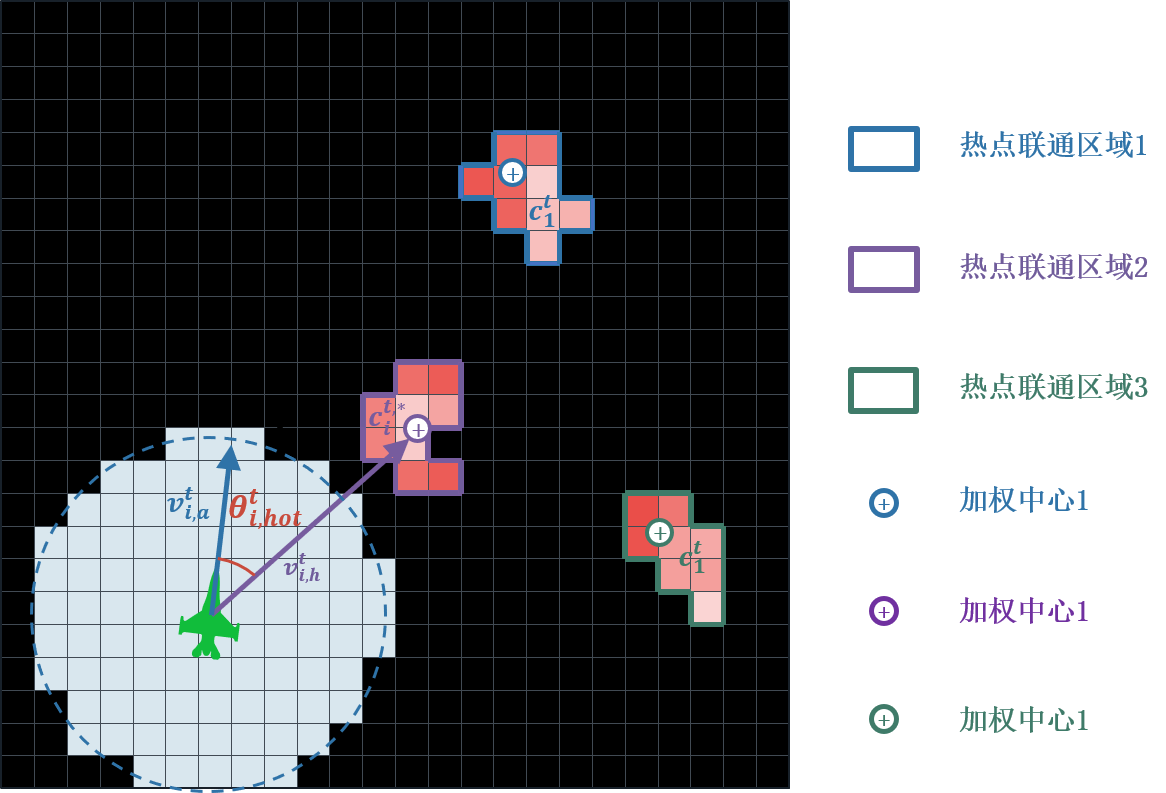
\includegraphics[width=0.75\textwidth]{热点区域中心示意图.png}
    \caption{热点连通域、概率加权中心与方向夹角示意}
    \label{fig:rec-hotspot-center-angle}
\end{figure}

信息阈值、高概率分割阈值和最小连通域面积分别用于判定低信息状态、提取热点和滤除噪声。

令无人机依据动作$a_i^t$形成的移动向量为
\begin{equation}
    \boldsymbol v_{i,\mathrm a}^t
    =\boldsymbol p_i^{t,\mathrm{next}}-\boldsymbol p_i^t,
\end{equation}
由当前位置指向热点中心的参考向量为
\begin{equation}
    \boldsymbol v_{i,\mathrm h}^t
    =\boldsymbol c_i^{t,*}-\boldsymbol p_i^t.
\end{equation}
两者夹角为
\begin{equation}
    \theta_{i,\mathrm{hot}}^t
    =
    \arccos
    \left(
    \frac{
    (\boldsymbol v_{i,\mathrm a}^t)^{\mathrm T}
    \boldsymbol v_{i,\mathrm h}^t}
    {
    \|\boldsymbol v_{i,\mathrm a}^t\|_2
    \|\boldsymbol v_{i,\mathrm h}^t\|_2}
    \right).
    \label{eq:rec-hotspot-angle}
\end{equation}
热点方向补偿奖励定义为
\begin{equation}
    r_{i,\mathrm{hot}}^t
    =
    \lambda_{\mathrm{hot}}
    \operatorname{clip}
    \left(
    \frac{\pi}{2}-\theta_{i,\mathrm{hot}}^t,
    -\frac{\pi}{2},
    \frac{\pi}{2}
    \right),
    \label{eq:rec-hotspot-direction-reward}
\end{equation}
其中$\lambda_{\mathrm{hot}}>0$。朝向、垂直和背离热点分别获得正、零和负奖励；低信息状态持续时保持目标以抑制振荡，恢复有效信息增益后停止补偿，不改变熵减奖励的主体地位。

\begingroup
\let\clearpage\relax
\chapter{原始数据附表}
\label{app:origin-data}
\endgroup

表~\ref{tab:raw-chapter3-search}--表~\ref{tab:raw-chapter5-upper}记录第三至第五章主要多场景对比实验的逐回合数据。$Cfg$为场景或参数配置，$M$为方法，$K$为指标；第三、第四章表头的$0$--$49$为同一配置下的独立测试序号，第五章表头的$31$--$60$为配对随机种子。同一场景、方法与指标的一行数据对应正文箱线图和统计检验使用的完整回合样本，未事后删除极端值。

指标口径与正文保持一致。第三章的目标发现比例取值为$[0,1]$，目标发现时间以决策步计，未发现目标按单回合最大决策步计入，回合平均信息熵取回合内全局信息熵在各决策步及其仿真子步上的平均值。第四、第五章的胜率、拦截率与损失率在附表中以$[0,1]$的比例记录；弹药利用效率为拦截数与弹药消耗量之比，平均拦截距离为拦截位置到保护中心的平均欧氏距离。回合奖励为对应章节所定义团队奖励的逐步累加，仅用于同一实验设置内的方法对比。各表的方法缩写和指标字母另在表后注释。

\begin{sidewaystable}[!htbp]
\captionsetup{font=footnotesize}
\caption{第三章搜索算法多场景测试原始数据}
\label{tab:raw-chapter3-search}
\centering
\begingroup
\fontsize{4.5pt}{5pt}\selectfont
\setlength{\tabcolsep}{0.6pt}
\renewcommand{\arraystretch}{0.75}
\begin{adjustbox}{max width=\linewidth}
\begin{tabular}{@{}lll*{50}{r}@{}}
\toprule
Cfg & M & K & 0 & 1 & 2 & 3 & 4 & 5 & 6 & 7 & 8 & 9 & 10 & 11 & 12 & 13 & 14 & 15 & 16 & 17 & 18 & 19 & 20 & 21 & 22 & 23 & 24 & 25 & 26 & 27 & 28 & 29 & 30 & 31 & 32 & 33 & 34 & 35 & 36 & 37 & 38 & 39 & 40 & 41 & 42 & 43 & 44 & 45 & 46 & 47 & 48 & 49 \\
\midrule
t12r3 & D & N & 0.750 & 0.583 & 0.667 & 0.667 & 0.583 & 0.833 & 0.583 & 0.833 & 0.583 & 0.833 & 0.667 & 0.667 & 0.667 & 0.833 & 0.667 & 0.667 & 0.500 & 0.583 & 0.500 & 0.750 & 0.583 & 0.583 & 0.917 & 0.583 & 0.833 & 0.833 & 0.667 & 0.750 & 0.417 & 0.750 & 0.917 & 0.583 & 0.833 & 0.750 & 0.667 & 0.833 & 0.750 & 0.750 & 0.583 & 0.667 & 0.583 & 0.500 & 0.750 & 0.667 & 0.583 & 0.500 & 0.750 & 0.667 & 0.917 & 0.583 \\
& D & T & 34.833 & 39.417 & 36.000 & 38.917 & 40.500 & 40.750 & 40.750 & 33.333 & 41.167 & 25.750 & 39.833 & 36.000 & 38.500 & 32.667 & 40.333 & 39.083 & 46.500 & 42.417 & 47.833 & 39.167 & 44.583 & 43.250 & 23.500 & 47.417 & 26.833 & 34.833 & 39.000 & 33.500 & 51.417 & 34.667 & 23.333 & 44.917 & 28.167 & 34.583 & 41.083 & 30.417 & 29.000 & 36.917 & 39.000 & 39.750 & 38.583 & 49.750 & 35.917 & 41.083 & 45.000 & 48.500 & 40.167 & 35.250 & 34.250 & 45.667 \\
& D & H & 192.836 & 199.967 & 213.256 & 263.238 & 153.863 & 252.227 & 202.156 & 225.057 & 194.386 & 178.691 & 224.894 & 203.409 & 241.058 & 221.906 & 222.223 & 246.492 & 248.375 & 229.303 & 220.802 & 192.981 & 191.385 & 205.383 & 214.483 & 233.632 & 193.688 & 233.088 & 245.770 & 247.425 & 225.985 & 176.949 & 183.858 & 232.591 & 210.056 & 219.476 & 212.344 & 190.705 & 184.747 & 228.956 & 262.808 & 229.085 & 189.198 & 219.332 & 189.134 & 217.740 & 215.459 & 196.786 & 172.790 & 193.314 & 242.829 & 244.917 \\
& M & N & 0.667 & 0.417 & 0.583 & 0.750 & 0.417 & 0.583 & 0.500 & 0.583 & 0.833 & 0.417 & 0.750 & 0.583 & 0.500 & 0.583 & 0.667 & 0.750 & 0.667 & 0.500 & 0.500 & 0.583 & 0.333 & 0.667 & 0.417 & 0.833 & 0.583 & 0.250 & 0.500 & 0.750 & 0.583 & 0.750 & 0.417 & 0.500 & 0.833 & 0.750 & 0.667 & 0.667 & 0.500 & 0.667 & 0.833 & 0.417 & 0.750 & 0.417 & 0.750 & 0.667 & 0.667 & 0.667 & 0.583 & 1.000 & 0.667 & 0.583 \\
& M & T & 44.583 & 61.417 & 43.167 & 40.250 & 56.083 & 51.250 & 68.417 & 59.417 & 41.000 & 58.083 & 46.667 & 49.917 & 58.083 & 47.917 & 40.333 & 47.000 & 47.333 & 58.000 & 51.083 & 44.667 & 69.000 & 55.333 & 54.417 & 43.167 & 41.833 & 64.750 & 56.250 & 45.167 & 50.833 & 51.333 & 56.333 & 54.583 & 45.833 & 41.250 & 48.167 & 42.833 & 52.833 & 42.917 & 34.583 & 56.917 & 34.750 & 63.333 & 50.750 & 48.833 & 41.500 & 55.000 & 46.500 & 46.750 & 48.917 & 52.500 \\
& M & H & 245.205 & 265.338 & 257.719 & 244.399 & 218.521 & 258.381 & 275.158 & 237.377 & 234.946 & 259.012 & 209.611 & 245.941 & 265.483 & 246.365 & 244.602 & 250.235 & 264.845 & 285.841 & 221.148 & 235.951 & 269.983 & 238.225 & 235.070 & 269.807 & 236.553 & 211.267 & 268.129 & 288.699 & 252.091 & 248.350 & 236.397 & 240.909 & 279.160 & 216.804 & 253.130 & 263.067 & 253.875 & 260.402 & 234.595 & 248.642 & 248.662 & 292.331 & 250.704 & 307.882 & 241.496 & 265.098 & 282.956 & 257.574 & 224.834 & 227.072 \\
& B & N & 0.667 & 0.500 & 0.417 & 0.667 & 0.667 & 0.500 & 0.750 & 0.333 & 0.417 & 0.417 & 0.417 & 0.667 & 0.250 & 0.083 & 0.500 & 0.500 & 0.750 & 0.500 & 0.333 & 0.333 & 0.167 & 0.250 & 0.500 & 0.583 & 0.250 & 0.667 & 0.417 & 0.583 & 0.583 & 0.417 & 0.667 & 0.667 & 0.417 & 0.500 & 0.417 & 0.333 & 0.583 & 0.333 & 0.583 & 0.333 & 0.417 & 0.583 & 0.833 & 0.583 & 0.500 & 0.500 & 0.583 & 0.417 & 0.333 & 0.750 \\
& B & T & 50.917 & 62.667 & 56.167 & 52.833 & 43.667 & 64.667 & 36.000 & 61.750 & 58.917 & 61.333 & 67.500 & 64.333 & 63.917 & 75.333 & 63.083 & 65.500 & 40.167 & 47.750 & 69.083 & 66.333 & 68.083 & 65.333 & 48.583 & 45.917 & 68.667 & 52.500 & 56.500 & 54.000 & 55.583 & 64.833 & 49.083 & 50.583 & 66.917 & 57.000 & 57.500 & 58.167 & 55.833 & 58.417 & 56.417 & 62.333 & 66.750 & 58.083 & 47.417 & 53.667 & 61.583 & 55.917 & 53.500 & 60.167 & 61.083 & 49.833 \\
& B & H & 237.766 & 296.468 & 284.530 & 242.346 & 268.848 & 317.587 & 237.088 & 288.222 & 315.463 & 299.685 & 314.771 & 304.354 & 323.490 & 324.549 & 320.662 & 322.635 & 238.873 & 266.999 & 322.652 & 319.112 & 323.661 & 310.840 & 306.352 & 234.389 & 336.886 & 233.208 & 267.741 & 268.958 & 276.776 & 256.589 & 271.546 & 271.572 & 330.566 & 266.191 & 287.853 & 303.129 & 237.418 & 330.768 & 235.618 & 315.902 & 323.929 & 270.494 & 231.392 & 292.141 & 310.391 & 284.413 & 306.111 & 283.684 & 329.051 & 236.158 \\
& I & N & 0.833 & 0.833 & 0.750 & 0.583 & 0.833 & 0.667 & 0.667 & 0.833 & 0.667 & 0.750 & 0.583 & 0.667 & 0.667 & 0.917 & 0.750 & 0.833 & 0.833 & 0.583 & 0.583 & 0.917 & 0.750 & 0.833 & 1.000 & 0.667 & 0.833 & 0.750 & 0.667 & 0.750 & 0.750 & 0.917 & 0.917 & 0.833 & 0.583 & 0.833 & 0.750 & 0.833 & 0.833 & 0.750 & 0.500 & 0.667 & 0.500 & 0.917 & 0.833 & 0.667 & 0.750 & 0.833 & 0.667 & 0.750 & 0.833 & 0.833 \\
& I & T & 38.333 & 48.250 & 44.583 & 52.000 & 35.000 & 39.000 & 42.500 & 35.667 & 43.750 & 51.750 & 44.000 & 50.833 & 44.167 & 33.000 & 40.917 & 30.750 & 39.667 & 42.250 & 65.167 & 31.000 & 48.167 & 45.583 & 25.417 & 40.083 & 42.250 & 28.167 & 41.500 & 39.667 & 52.500 & 31.500 & 31.167 & 32.000 & 46.333 & 33.667 & 47.167 & 32.167 & 38.667 & 37.333 & 49.500 & 50.500 & 54.833 & 32.500 & 27.333 & 43.750 & 53.833 & 42.583 & 43.500 & 43.167 & 26.250 & 41.250 \\
& I & H & 195.790 & 231.838 & 210.467 & 215.304 & 189.593 & 266.891 & 212.707 & 229.841 & 228.472 & 230.870 & 256.399 & 245.744 & 227.435 & 216.574 & 241.038 & 210.802 & 165.443 & 192.865 & 252.880 & 195.237 & 209.883 & 216.879 & 213.670 & 250.242 & 177.590 & 243.139 & 164.580 & 235.047 & 167.406 & 220.735 & 201.887 & 209.170 & 185.375 & 199.058 & 235.443 & 206.038 & 248.230 & 228.140 & 250.547 & 235.221 & 232.549 & 227.070 & 224.763 & 179.486 & 235.791 & 180.072 & 270.200 & 223.727 & 230.778 & 199.594 \\
& P & N & 0.917 & 0.750 & 0.500 & 0.667 & 0.917 & 0.833 & 0.750 & 0.917 & 0.667 & 0.500 & 0.750 & 0.667 & 0.500 & 0.750 & 0.667 & 0.833 & 0.750 & 0.917 & 0.750 & 0.750 & 0.833 & 0.750 & 0.833 & 0.583 & 0.500 & 0.917 & 0.750 & 0.917 & 0.833 & 0.750 & 0.500 & 0.750 & 0.750 & 0.667 & 0.500 & 0.667 & 0.750 & 0.917 & 0.833 & 0.667 & 0.750 & 0.667 & 0.833 & 0.667 & 0.750 & 0.667 & 0.583 & 0.833 & 0.667 & 0.667 \\
& P & T & 30.000 & 53.833 & 51.417 & 41.333 & 34.250 & 36.750 & 43.250 & 33.000 & 52.083 & 51.167 & 42.000 & 39.833 & 49.417 & 41.083 & 41.917 & 42.750 & 39.250 & 41.583 & 39.500 & 31.500 & 41.750 & 41.083 & 33.000 & 51.750 & 58.000 & 27.167 & 45.917 & 24.333 & 29.000 & 44.667 & 48.750 & 47.750 & 38.917 & 43.500 & 57.250 & 51.000 & 37.583 & 34.083 & 38.583 & 49.333 & 41.000 & 50.667 & 49.333 & 46.000 & 35.250 & 52.750 & 46.083 & 36.417 & 37.583 & 49.250 \\
& P & H & 211.116 & 190.276 & 235.292 & 249.727 & 236.822 & 220.021 & 205.071 & 169.419 & 227.612 & 187.825 & 232.281 & 253.389 & 243.851 & 204.731 & 181.592 & 216.527 & 213.352 & 237.409 & 184.545 & 230.890 & 225.494 & 195.139 & 178.114 & 203.051 & 293.903 & 239.368 & 220.755 & 201.484 & 205.832 & 245.981 & 281.000 & 216.490 & 278.444 & 231.838 & 232.302 & 203.219 & 218.922 & 205.202 & 228.859 & 228.984 & 243.233 & 201.898 & 216.212 & 224.227 & 190.240 & 254.900 & 252.991 & 193.321 & 218.364 & 233.617 \\
& T & N & 0.417 & 0.833 & 0.833 & 0.333 & 0.417 & 0.750 & 0.750 & 0.750 & 0.667 & 0.750 & 0.750 & 0.750 & 0.833 & 0.833 & 0.500 & 0.833 & 0.583 & 0.750 & 0.667 & 0.750 & 0.667 & 0.583 & 0.833 & 0.583 & 0.500 & 0.833 & 0.500 & 0.750 & 0.583 & 0.833 & 0.833 & 0.667 & 0.667 & 0.667 & 0.917 & 0.750 & 0.667 & 0.750 & 0.750 & 0.833 & 0.583 & 0.750 & 0.500 & 0.667 & 0.667 & 0.750 & 0.750 & 0.500 & 0.667 & 0.833 \\
& T & T & 53.333 & 43.417 & 48.333 & 56.333 & 58.000 & 41.583 & 40.333 & 46.917 & 39.167 & 30.250 & 36.667 & 42.333 & 45.167 & 28.167 & 53.750 & 36.083 & 42.750 & 39.500 & 39.083 & 41.667 & 46.250 & 50.833 & 35.667 & 50.667 & 43.750 & 36.083 & 55.667 & 35.917 & 51.833 & 32.500 & 31.083 & 40.167 & 51.167 & 52.000 & 34.167 & 46.250 & 51.167 & 44.333 & 38.833 & 37.417 & 44.417 & 38.250 & 52.000 & 47.750 & 43.500 & 43.083 & 41.500 & 58.333 & 44.000 & 41.417 \\
& T & H & 263.975 & 240.877 & 212.425 & 193.645 & 260.953 & 256.101 & 183.739 & 257.818 & 182.802 & 231.080 & 218.863 & 240.341 & 200.791 & 182.383 & 249.937 & 202.060 & 202.871 & 207.121 & 214.420 & 207.078 & 215.728 & 230.492 & 207.432 & 209.412 & 217.349 & 186.155 & 245.856 & 190.687 & 215.530 & 200.540 & 258.247 & 232.411 & 211.173 & 225.058 & 181.453 & 221.692 & 258.294 & 236.831 & 209.833 & 235.181 & 224.397 & 233.246 & 225.537 & 184.747 & 252.231 & 259.376 & 216.439 & 234.823 & 208.312 & 213.973 \\
t12r6 & D & N & 0.750 & 0.833 & 0.917 & 0.833 & 0.750 & 0.917 & 0.917 & 0.667 & 0.833 & 1.000 & 0.750 & 0.917 & 0.833 & 0.833 & 1.000 & 0.667 & 0.917 & 0.917 & 0.917 & 0.917 & 0.667 & 0.833 & 0.833 & 0.750 & 1.000 & 0.750 & 1.000 & 0.750 & 0.833 & 0.833 & 0.833 & 0.833 & 0.833 & 1.000 & 1.000 & 0.917 & 1.000 & 0.917 & 1.000 & 1.000 & 0.917 & 0.833 & 0.750 & 0.750 & 0.833 & 0.667 & 0.833 & 1.000 & 0.917 & 0.917 \\
& D & T & 28.750 & 35.000 & 33.833 & 30.750 & 35.000 & 30.000 & 25.083 & 34.083 & 30.167 & 16.667 & 33.083 & 24.750 & 32.083 & 27.583 & 26.917 & 36.917 & 24.917 & 19.833 & 25.083 & 29.083 & 39.500 & 26.667 & 29.917 & 36.917 & 16.250 & 35.250 & 22.750 & 31.917 & 27.083 & 34.250 & 31.667 & 25.333 & 22.250 & 23.083 & 20.250 & 23.417 & 24.000 & 22.833 & 22.083 & 11.583 & 22.083 & 27.083 & 32.000 & 30.167 & 32.667 & 35.333 & 26.833 & 22.250 & 21.750 & 22.667 \\
& D & H & 186.235 & 216.280 & 224.171 & 174.725 & 177.151 & 167.591 & 124.657 & 203.942 & 197.071 & 214.070 & 176.938 & 149.883 & 190.485 & 164.871 & 170.936 & 185.587 & 161.771 & 186.102 & 167.054 & 180.219 & 215.924 & 185.757 & 205.905 & 156.693 & 129.101 & 167.079 & 205.436 & 198.236 & 184.090 & 181.158 & 154.677 & 212.341 & 190.396 & 191.923 & 184.021 & 144.038 & 220.661 & 183.296 & 196.139 & 187.711 & 188.017 & 195.021 & 163.088 & 170.918 & 189.579 & 163.805 & 165.042 & 197.249 & 173.055 & 185.722 \\
& M & N & 0.500 & 0.583 & 0.750 & 0.750 & 0.750 & 0.833 & 0.500 & 0.583 & 0.667 & 0.917 & 0.583 & 0.833 & 0.833 & 0.917 & 0.583 & 0.500 & 0.917 & 0.750 & 0.667 & 0.833 & 0.250 & 0.917 & 0.417 & 0.750 & 0.583 & 0.667 & 0.917 & 0.667 & 0.917 & 0.750 & 0.750 & 0.833 & 0.583 & 0.417 & 0.917 & 0.833 & 1.000 & 0.667 & 0.750 & 0.583 & 0.833 & 0.750 & 0.667 & 0.750 & 0.583 & 0.833 & 1.000 & 0.417 & 0.750 & 0.667 \\
& M & T & 63.500 & 52.750 & 53.583 & 39.417 & 38.167 & 30.667 & 50.417 & 53.750 & 49.167 & 34.000 & 60.417 & 47.250 & 37.833 & 43.833 & 50.500 & 55.250 & 41.417 & 50.750 & 49.333 & 43.250 & 65.083 & 44.000 & 65.667 & 42.583 & 50.833 & 58.250 & 54.583 & 47.833 & 30.750 & 48.417 & 46.333 & 45.250 & 47.833 & 60.250 & 31.500 & 39.917 & 29.583 & 51.833 & 40.917 & 45.500 & 40.750 & 49.250 & 50.917 & 47.750 & 43.583 & 37.000 & 28.583 & 57.833 & 52.250 & 52.750 \\
& M & H & 241.292 & 230.075 & 226.682 & 197.846 & 221.691 & 214.388 & 250.863 & 226.364 & 225.960 & 252.880 & 222.102 & 243.630 & 238.644 & 218.850 & 238.014 & 276.488 & 221.211 & 190.546 & 257.711 & 170.158 & 258.982 & 190.777 & 223.348 & 235.651 & 253.580 & 228.851 & 263.605 & 221.764 & 186.576 & 250.456 & 232.152 & 241.536 & 246.695 & 249.653 & 210.061 & 227.410 & 222.776 & 277.462 & 219.237 & 237.728 & 208.359 & 240.986 & 220.173 & 220.898 & 227.192 & 242.063 & 183.096 & 202.025 & 267.907 & 270.274 \\
& B & N & 1.000 & 0.417 & 0.750 & 0.833 & 0.417 & 0.500 & 0.833 & 0.833 & 0.833 & 0.417 & 0.667 & 0.417 & 0.750 & 0.667 & 0.500 & 0.833 & 0.750 & 0.750 & 0.917 & 0.833 & 0.750 & 1.000 & 0.583 & 0.500 & 0.667 & 1.000 & 0.333 & 0.167 & 0.333 & 0.750 & 0.917 & 0.917 & 0.917 & 0.583 & 0.167 & 0.167 & 0.333 & 0.833 & 0.583 & 0.917 & 0.417 & 1.000 & 0.500 & 0.417 & 0.583 & 0.917 & 0.833 & 0.667 & 0.750 & 0.750 \\
& B & T & 29.167 & 53.083 & 50.833 & 42.917 & 63.000 & 49.083 & 33.917 & 40.500 & 40.417 & 54.083 & 40.333 & 54.500 & 45.500 & 45.917 & 55.167 & 56.417 & 40.917 & 59.000 & 31.167 & 44.583 & 40.500 & 31.250 & 53.083 & 55.083 & 43.417 & 30.833 & 63.583 & 72.250 & 61.500 & 49.833 & 46.167 & 31.917 & 40.917 & 48.250 & 68.667 & 74.083 & 69.917 & 52.667 & 50.500 & 31.917 & 61.667 & 27.917 & 49.250 & 59.750 & 51.750 & 28.667 & 35.667 & 55.667 & 44.500 & 47.500 \\
& B & H & 180.360 & 249.641 & 249.385 & 211.238 & 239.535 & 190.560 & 187.206 & 219.429 & 208.134 & 210.285 & 221.050 & 191.025 & 246.582 & 261.889 & 289.595 & 290.936 & 239.161 & 273.134 & 202.456 & 218.001 & 237.577 & 166.749 & 234.720 & 187.149 & 216.070 & 201.739 & 265.748 & 316.867 & 284.915 & 256.296 & 233.979 & 240.704 & 214.532 & 183.759 & 329.865 & 307.847 & 308.983 & 245.792 & 234.474 & 244.672 & 280.487 & 218.598 & 177.873 & 275.471 & 218.688 & 184.789 & 200.183 & 233.078 & 214.280 & 223.016 \\
& I & N & 0.833 & 0.750 & 0.917 & 0.833 & 1.000 & 1.000 & 0.833 & 1.000 & 1.000 & 1.000 & 0.917 & 1.000 & 0.833 & 1.000 & 0.750 & 0.917 & 0.833 & 0.833 & 0.917 & 0.833 & 0.833 & 0.833 & 0.833 & 0.917 & 0.833 & 0.917 & 0.833 & 0.833 & 1.000 & 1.000 & 1.000 & 0.750 & 0.917 & 1.000 & 1.000 & 0.917 & 0.917 & 0.917 & 0.833 & 0.833 & 0.833 & 0.833 & 0.917 & 0.833 & 0.833 & 0.917 & 1.000 & 1.000 & 0.833 & 0.667 \\
& I & T & 27.917 & 37.583 & 27.917 & 30.917 & 29.583 & 13.333 & 31.917 & 22.083 & 23.750 & 18.417 & 30.417 & 26.250 & 33.083 & 19.333 & 33.333 & 34.000 & 33.667 & 32.583 & 22.750 & 30.667 & 33.500 & 26.333 & 38.250 & 29.917 & 28.833 & 20.417 & 23.667 & 34.167 & 17.167 & 18.583 & 23.333 & 34.250 & 33.417 & 20.667 & 17.833 & 30.417 & 24.917 & 27.167 & 28.667 & 30.417 & 29.917 & 42.917 & 22.250 & 27.167 & 27.750 & 20.417 & 23.167 & 21.333 & 27.000 & 41.250 \\
& I & H & 162.289 & 162.818 & 190.801 & 190.089 & 183.944 & 209.960 & 157.710 & 162.638 & 129.224 & 134.920 & 152.827 & 185.942 & 143.539 & 169.627 & 136.956 & 160.997 & 191.178 & 155.089 & 171.217 & 159.888 & 180.804 & 175.763 & 166.993 & 155.114 & 141.581 & 125.216 & 159.359 & 216.875 & 183.239 & 194.477 & 171.476 & 140.781 & 143.786 & 177.466 & 198.668 & 140.298 & 148.719 & 154.083 & 132.282 & 187.552 & 141.419 & 158.803 & 183.754 & 181.013 & 114.566 & 161.102 & 167.401 & 166.974 & 144.453 & 193.799 \\
& P & N & 0.833 & 0.750 & 0.833 & 0.750 & 0.833 & 0.833 & 0.833 & 0.917 & 0.833 & 1.000 & 0.833 & 1.000 & 0.917 & 0.917 & 1.000 & 0.750 & 1.000 & 0.833 & 0.917 & 1.000 & 0.750 & 0.833 & 0.833 & 0.833 & 0.917 & 0.833 & 0.833 & 0.750 & 1.000 & 1.000 & 0.833 & 0.917 & 0.833 & 0.917 & 0.833 & 0.833 & 0.750 & 0.750 & 0.667 & 0.833 & 1.000 & 0.667 & 0.917 & 0.917 & 0.750 & 1.000 & 0.833 & 1.000 & 0.667 & 0.833 \\
& P & T & 36.667 & 37.333 & 44.667 & 49.167 & 43.667 & 27.667 & 36.917 & 28.583 & 28.667 & 24.083 & 31.000 & 26.083 & 31.083 & 35.083 & 31.417 & 44.167 & 24.750 & 34.250 & 31.583 & 33.083 & 30.167 & 45.250 & 39.000 & 33.833 & 33.417 & 33.917 & 33.500 & 39.500 & 27.167 & 29.583 & 37.000 & 28.167 & 37.583 & 27.833 & 32.000 & 41.083 & 38.417 & 45.500 & 53.500 & 35.417 & 26.750 & 48.250 & 33.083 & 25.417 & 44.917 & 31.583 & 32.833 & 31.250 & 44.917 & 36.417 \\
& P & H & 197.411 & 217.496 & 212.375 & 246.674 & 199.710 & 191.838 & 147.603 & 178.820 & 172.897 & 190.669 & 177.130 & 201.150 & 140.623 & 194.319 & 193.964 & 182.963 & 159.483 & 192.453 & 174.036 & 170.126 & 148.947 & 195.591 & 174.101 & 165.705 & 157.690 & 175.267 & 170.278 & 196.588 & 136.955 & 171.248 & 176.672 & 188.213 & 221.511 & 164.452 & 145.616 & 176.098 & 222.106 & 178.988 & 171.609 & 196.461 & 146.760 & 220.087 & 178.092 & 187.307 & 220.618 & 185.866 & 150.973 & 173.005 & 214.636 & 225.994 \\
& T & N & 0.917 & 0.750 & 0.917 & 0.917 & 0.667 & 0.750 & 0.833 & 0.833 & 0.917 & 0.917 & 0.750 & 0.917 & 0.750 & 0.917 & 0.750 & 0.833 & 1.000 & 0.917 & 1.000 & 0.917 & 0.917 & 1.000 & 0.750 & 0.917 & 0.917 & 0.833 & 0.833 & 0.750 & 0.917 & 0.833 & 0.833 & 0.750 & 0.917 & 0.917 & 0.750 & 1.000 & 0.833 & 0.750 & 0.750 & 0.917 & 0.833 & 0.833 & 0.833 & 0.667 & 0.750 & 0.750 & 0.667 & 0.750 & 0.833 & 1.000 \\
& T & T & 38.917 & 41.417 & 31.500 & 28.667 & 52.500 & 43.667 & 39.833 & 37.417 & 22.417 & 28.167 & 32.500 & 29.250 & 37.417 & 24.667 & 31.583 & 34.000 & 32.167 & 28.500 & 28.583 & 46.583 & 34.000 & 20.000 & 35.250 & 35.000 & 37.833 & 36.083 & 33.667 & 36.167 & 29.250 & 33.667 & 41.417 & 38.750 & 34.917 & 31.083 & 38.833 & 34.250 & 39.417 & 40.167 & 38.667 & 34.000 & 44.917 & 36.833 & 40.500 & 39.500 & 36.000 & 53.000 & 43.500 & 44.917 & 44.083 & 23.000 \\
& T & H & 227.723 & 181.964 & 164.793 & 179.251 & 182.990 & 177.587 & 165.268 & 149.097 & 162.028 & 195.549 & 130.998 & 228.617 & 179.562 & 205.446 & 196.185 & 230.161 & 198.364 & 194.574 & 202.238 & 172.748 & 211.602 & 200.812 & 195.835 & 149.968 & 211.315 & 184.542 & 162.943 & 190.648 & 186.073 & 172.980 & 240.253 & 173.524 & 202.517 & 212.840 & 229.118 & 191.264 & 203.068 & 220.036 & 170.430 & 175.513 & 172.115 & 205.013 & 186.913 & 213.322 & 170.429 & 193.878 & 210.358 & 150.530 & 180.230 & 213.552 \\
t15r3 & D & N & 0.867 & 0.800 & 0.600 & 0.533 & 0.733 & 0.800 & 0.800 & 0.667 & 0.600 & 0.200 & 0.667 & 0.800 & 0.800 & 0.600 & 0.667 & 0.533 & 0.600 & 0.667 & 0.600 & 0.733 & 0.400 & 0.667 & 0.600 & 0.867 & 0.667 & 0.733 & 0.733 & 0.667 & 0.600 & 0.667 & 0.600 & 0.667 & 0.600 & 0.867 & 0.800 & 0.867 & 0.800 & 0.600 & 0.733 & 0.600 & 0.533 & 0.733 & 0.600 & 0.467 & 0.667 & 0.533 & 0.600 & 0.600 & 0.667 & 0.467 \\
& D & T & 25.667 & 30.067 & 44.400 & 43.667 & 33.933 & 28.333 & 29.067 & 42.467 & 41.800 & 65.000 & 39.267 & 31.133 & 27.667 & 43.533 & 38.667 & 44.867 & 38.133 & 45.600 & 40.667 & 36.867 & 51.733 & 41.533 & 43.000 & 25.133 & 39.333 & 35.133 & 33.467 & 38.200 & 41.733 & 42.333 & 52.533 & 40.533 & 47.267 & 27.667 & 31.533 & 25.867 & 32.800 & 42.933 & 30.733 & 41.533 & 52.133 & 33.333 & 42.933 & 50.467 & 35.267 & 45.333 & 46.533 & 42.667 & 41.933 & 48.333 \\
& D & H & 237.244 & 236.728 & 269.184 & 301.616 & 253.111 & 222.775 & 290.094 & 270.574 & 272.819 & 329.877 & 250.956 & 272.107 & 219.442 & 209.525 & 269.289 & 273.427 & 338.879 & 244.169 & 257.513 & 307.861 & 325.024 & 275.841 & 254.772 & 207.621 & 270.440 & 255.764 & 296.433 & 235.691 & 281.874 & 280.137 & 269.090 & 226.059 & 271.754 & 242.433 & 235.673 & 220.034 & 243.659 & 251.563 & 290.722 & 303.974 & 323.495 & 280.217 & 276.870 & 263.657 & 302.881 & 256.659 & 268.354 & 278.762 & 268.272 & 303.081 \\
& M & N & 0.467 & 0.533 & 0.667 & 0.467 & 0.400 & 0.533 & 0.533 & 0.733 & 0.533 & 0.733 & 0.600 & 0.933 & 0.733 & 0.600 & 0.600 & 0.600 & 0.600 & 0.533 & 0.733 & 0.533 & 0.467 & 0.600 & 0.533 & 0.333 & 0.400 & 0.533 & 0.533 & 0.533 & 0.600 & 0.667 & 0.600 & 0.667 & 0.733 & 0.800 & 0.600 & 0.400 & 0.467 & 0.400 & 0.600 & 0.467 & 0.533 & 0.533 & 0.800 & 0.533 & 0.867 & 0.667 & 0.800 & 0.400 & 0.733 & 0.467 \\
& M & T & 60.733 & 52.800 & 47.000 & 56.200 & 55.533 & 59.533 & 49.467 & 36.867 & 50.867 & 42.000 & 42.800 & 37.467 & 37.067 & 43.733 & 49.733 & 50.200 & 44.733 & 55.400 & 43.067 & 56.533 & 59.000 & 42.067 & 51.000 & 60.467 & 60.533 & 49.467 & 62.067 & 52.667 & 53.800 & 42.667 & 51.933 & 52.467 & 41.933 & 36.733 & 43.533 & 60.867 & 59.133 & 58.133 & 48.067 & 51.800 & 57.467 & 48.867 & 41.867 & 48.533 & 39.200 & 48.667 & 46.667 & 56.200 & 37.067 & 49.800 \\
& M & H & 287.898 & 257.616 & 286.784 & 273.939 & 321.829 & 253.771 & 275.452 & 241.375 & 260.680 & 260.373 & 297.196 & 254.961 & 262.929 & 297.154 & 331.786 & 243.869 & 254.895 & 304.016 & 265.625 & 282.279 & 300.473 & 240.084 & 322.405 & 323.395 & 241.957 & 333.786 & 303.932 & 280.829 & 329.045 & 285.091 & 343.239 & 325.663 & 271.898 & 252.223 & 263.706 & 275.113 & 320.266 & 255.185 & 285.099 & 275.861 & 286.598 & 263.057 & 312.801 & 253.190 & 285.793 & 296.179 & 291.076 & 293.742 & 291.913 & 293.010 \\
& B & N & 0.733 & 0.333 & 0.200 & 0.467 & 0.200 & 0.333 & 0.267 & 0.267 & 0.333 & 0.400 & 0.267 & 0.400 & 0.333 & 0.333 & 0.333 & 0.267 & 0.400 & 0.200 & 0.267 & 0.133 & 0.400 & 0.333 & 0.467 & 0.733 & 0.267 & 0.333 & 0.400 & 0.600 & 0.267 & 0.600 & 0.333 & 0.400 & 0.267 & 0.467 & 0.400 & 0.400 & 0.267 & 0.267 & 0.333 & 0.533 & 0.200 & 0.600 & 0.200 & 0.467 & 0.467 & 0.333 & 0.667 & 0.467 & 0.267 & 0.333 \\
& B & T & 59.200 & 64.933 & 71.600 & 52.733 & 68.667 & 61.267 & 67.133 & 63.533 & 58.800 & 63.400 & 68.600 & 57.200 & 57.267 & 62.267 & 64.867 & 66.333 & 59.733 & 67.200 & 62.000 & 69.800 & 56.133 & 59.600 & 60.467 & 45.533 & 63.933 & 61.733 & 56.667 & 45.067 & 67.400 & 51.533 & 63.467 & 61.067 & 64.067 & 58.733 & 57.533 & 59.800 & 70.000 & 62.600 & 63.600 & 54.267 & 67.400 & 53.200 & 67.733 & 65.133 & 56.600 & 60.333 & 54.800 & 65.067 & 69.400 & 64.400 \\
& B & H & 308.042 & 380.339 & 328.688 & 358.457 & 383.536 & 364.618 & 396.841 & 334.116 & 301.988 & 392.385 & 331.050 & 308.038 & 385.086 & 324.105 & 342.731 & 375.342 & 367.206 & 345.872 & 306.834 & 366.504 & 335.665 & 295.253 & 331.195 & 286.553 & 347.369 & 327.499 & 299.042 & 294.296 & 346.108 & 302.686 & 369.289 & 357.652 & 329.640 & 297.559 & 321.662 & 317.901 & 335.952 & 317.076 & 309.207 & 345.826 & 358.220 & 294.892 & 367.990 & 337.620 & 315.366 & 287.510 & 336.280 & 369.815 & 353.748 & 332.883 \\
& I & N & 0.733 & 0.467 & 0.467 & 0.600 & 0.533 & 0.733 & 0.533 & 0.733 & 0.800 & 0.600 & 0.667 & 0.800 & 0.733 & 0.733 & 0.667 & 0.733 & 0.733 & 0.467 & 0.533 & 0.733 & 0.533 & 0.800 & 0.867 & 0.533 & 0.800 & 0.600 & 0.733 & 0.733 & 0.867 & 0.600 & 0.933 & 0.400 & 0.933 & 0.800 & 0.533 & 0.800 & 0.733 & 0.733 & 0.867 & 0.600 & 0.867 & 0.533 & 0.733 & 0.733 & 0.533 & 0.733 & 0.533 & 0.733 & 0.800 & 0.600 \\
& I & T & 41.400 & 54.467 & 50.733 & 45.267 & 45.600 & 39.267 & 53.467 & 42.267 & 34.333 & 42.200 & 48.867 & 46.133 & 38.867 & 36.400 & 41.533 & 38.400 & 45.000 & 52.867 & 49.533 & 52.267 & 48.667 & 44.933 & 36.800 & 45.067 & 40.200 & 47.400 & 38.600 & 40.267 & 37.467 & 53.133 & 33.800 & 56.933 & 38.133 & 37.200 & 55.800 & 39.533 & 39.733 & 43.467 & 41.400 & 50.867 & 34.200 & 47.600 & 48.200 & 41.400 & 48.867 & 43.867 & 50.133 & 45.933 & 39.267 & 43.200 \\
& I & H & 294.656 & 268.648 & 279.199 & 279.870 & 267.161 & 274.224 & 237.719 & 284.631 & 242.457 & 251.452 & 275.221 & 278.854 & 261.682 & 227.901 & 260.314 & 237.728 & 263.801 & 285.280 & 293.876 & 269.065 & 275.896 & 274.752 & 223.423 & 236.013 & 252.947 & 294.777 & 242.286 & 273.433 & 214.732 & 274.949 & 299.021 & 323.640 & 205.050 & 258.272 & 253.866 & 269.010 & 250.323 & 198.242 & 251.435 & 284.375 & 281.281 & 294.961 & 237.888 & 221.484 & 256.129 & 190.392 & 264.696 & 213.032 & 264.515 & 241.572 \\
& P & N & 0.933 & 0.667 & 0.600 & 0.667 & 0.800 & 0.667 & 0.600 & 0.667 & 0.733 & 0.800 & 0.667 & 0.667 & 0.600 & 0.867 & 0.867 & 0.733 & 0.400 & 0.600 & 0.533 & 0.600 & 0.600 & 0.600 & 0.600 & 0.533 & 0.667 & 0.800 & 0.533 & 0.533 & 0.533 & 0.733 & 0.533 & 0.533 & 0.667 & 0.800 & 0.800 & 0.733 & 0.467 & 0.733 & 0.600 & 0.800 & 0.600 & 0.600 & 0.467 & 0.667 & 0.800 & 0.867 & 0.733 & 0.867 & 0.733 & 0.667 \\
& P & T & 32.067 & 41.133 & 49.067 & 40.600 & 46.800 & 39.533 & 45.267 & 49.400 & 40.333 & 34.267 & 38.933 & 35.733 & 49.533 & 30.733 & 33.600 & 40.800 & 58.267 & 47.467 & 51.133 & 53.000 & 45.667 & 40.200 & 43.867 & 42.667 & 45.400 & 40.800 & 49.733 & 48.533 & 49.800 & 38.733 & 51.333 & 51.200 & 50.867 & 41.600 & 37.800 & 44.933 & 52.067 & 40.200 & 41.067 & 41.067 & 38.733 & 45.533 & 47.600 & 41.800 & 35.200 & 33.733 & 35.533 & 33.733 & 34.800 & 42.933 \\
& P & H & 237.435 & 253.839 & 221.531 & 268.872 & 270.477 & 247.070 & 274.047 & 262.588 & 234.706 & 266.080 & 293.745 & 222.825 & 287.268 & 268.710 & 269.995 & 243.872 & 288.363 & 259.224 & 227.495 & 295.203 & 263.056 & 280.896 & 326.087 & 295.137 & 246.218 & 220.693 & 220.257 & 221.898 & 237.793 & 277.022 & 277.049 & 312.039 & 264.623 & 313.325 & 283.794 & 249.154 & 241.658 & 259.799 & 278.771 & 248.977 & 291.201 & 308.664 & 250.801 & 255.743 & 253.317 & 262.082 & 273.727 & 228.186 & 271.022 & 291.810 \\
& T & N & 0.600 & 0.733 & 0.533 & 0.600 & 0.533 & 0.467 & 0.600 & 0.600 & 0.733 & 0.733 & 0.733 & 0.733 & 0.867 & 0.667 & 0.533 & 0.600 & 0.733 & 0.733 & 0.667 & 0.533 & 0.467 & 0.600 & 0.533 & 0.800 & 0.800 & 0.667 & 0.600 & 0.667 & 0.600 & 0.467 & 0.733 & 0.667 & 0.533 & 0.667 & 0.667 & 0.867 & 0.600 & 0.600 & 0.467 & 0.400 & 0.667 & 0.600 & 0.667 & 0.467 & 0.600 & 0.667 & 0.533 & 0.600 & 0.667 & 0.600 \\
& T & T & 40.933 & 42.667 & 47.333 & 40.933 & 54.667 & 55.000 & 41.333 & 52.933 & 43.733 & 46.800 & 44.000 & 39.133 & 51.867 & 44.267 & 52.067 & 47.267 & 49.333 & 36.533 & 55.867 & 53.933 & 59.200 & 46.000 & 49.800 & 44.933 & 39.533 & 44.000 & 39.467 & 44.267 & 45.000 & 57.733 & 47.867 & 48.200 & 47.667 & 49.467 & 51.400 & 31.733 & 56.267 & 44.333 & 51.533 & 64.067 & 50.267 & 44.467 & 45.200 & 58.000 & 48.933 & 36.933 & 51.333 & 50.933 & 52.067 & 44.067 \\
& T & H & 283.702 & 265.816 & 314.823 & 255.418 & 318.957 & 277.284 & 268.684 & 306.436 & 283.877 & 303.572 & 220.377 & 251.738 & 292.091 & 292.396 & 232.948 & 248.515 & 277.081 & 288.375 & 292.163 & 248.510 & 249.807 & 250.444 & 252.453 & 291.652 & 263.723 & 266.019 & 230.100 & 261.402 & 225.651 & 294.725 & 231.771 & 308.713 & 268.728 & 290.599 & 298.228 & 200.607 & 273.681 & 308.785 & 299.776 & 318.109 & 295.401 & 261.616 & 261.015 & 296.739 & 317.432 & 258.849 & 262.313 & 262.150 & 261.539 & 265.751 \\
t18r6 & D & N & 0.722 & 0.778 & 0.833 & 0.778 & 0.556 & 0.889 & 0.944 & 0.667 & 0.722 & 0.722 & 0.889 & 0.833 & 0.556 & 0.778 & 0.944 & 0.722 & 0.722 & 0.667 & 0.667 & 0.833 & 0.722 & 0.833 & 0.611 & 0.833 & 0.778 & 0.778 & 0.833 & 0.833 & 0.722 & 0.667 & 0.833 & 0.722 & 0.833 & 0.667 & 0.722 & 0.889 & 0.778 & 0.778 & 0.944 & 0.611 & 0.778 & 0.556 & 0.833 & 0.722 & 0.778 & 0.833 & 0.722 & 0.889 & 0.556 & 0.833 \\
& D & T & 35.667 & 30.500 & 27.833 & 36.611 & 45.833 & 19.333 & 26.389 & 35.611 & 35.167 & 32.667 & 25.722 & 28.722 & 44.111 & 34.667 & 22.667 & 35.944 & 31.111 & 40.167 & 37.333 & 22.111 & 36.889 & 29.944 & 46.389 & 33.278 & 28.222 & 31.111 & 32.333 & 31.444 & 32.833 & 40.667 & 22.944 & 36.778 & 29.778 & 34.611 & 37.389 & 20.889 & 33.389 & 34.167 & 23.833 & 38.889 & 31.722 & 45.056 & 31.000 & 34.944 & 35.722 & 27.222 & 31.056 & 24.611 & 44.889 & 27.611 \\
& D & H & 242.822 & 250.703 & 235.761 & 279.563 & 272.823 & 276.209 & 256.022 & 279.185 & 236.399 & 282.528 & 179.216 & 284.620 & 323.846 & 286.076 & 225.660 & 283.089 & 239.962 & 246.934 & 257.896 & 268.844 & 281.569 & 247.146 & 223.607 & 256.213 & 289.623 & 257.723 & 234.319 & 238.643 & 291.981 & 227.993 & 254.699 & 205.206 & 261.817 & 272.128 & 260.877 & 184.633 & 247.640 & 266.954 & 229.863 & 282.178 & 265.770 & 302.253 & 244.041 & 328.645 & 236.510 & 261.313 & 273.937 & 230.237 & 243.215 & 225.922 \\
& M & N & 0.611 & 0.667 & 0.667 & 0.833 & 0.444 & 0.611 & 0.611 & 0.722 & 0.500 & 0.667 & 0.667 & 0.667 & 0.556 & 0.611 & 0.500 & 0.500 & 0.833 & 0.611 & 0.333 & 0.722 & 0.778 & 0.889 & 0.667 & 0.611 & 0.944 & 0.833 & 0.611 & 0.556 & 0.778 & 0.778 & 0.833 & 0.667 & 0.667 & 0.500 & 0.944 & 0.722 & 0.778 & 0.889 & 0.944 & 0.722 & 0.778 & 0.889 & 0.556 & 0.611 & 0.722 & 0.611 & 0.667 & 0.833 & 0.667 & 0.444 \\
& M & T & 53.889 & 45.722 & 44.667 & 34.556 & 54.000 & 49.778 & 45.500 & 41.056 & 61.667 & 45.667 & 47.444 & 51.778 & 49.889 & 55.722 & 58.444 & 58.833 & 39.944 & 53.222 & 62.556 & 44.556 & 50.944 & 36.944 & 48.111 & 53.056 & 28.556 & 38.889 & 54.500 & 51.833 & 38.667 & 45.000 & 41.778 & 42.111 & 49.278 & 55.000 & 33.611 & 33.722 & 36.222 & 40.278 & 37.833 & 44.611 & 44.167 & 36.389 & 46.778 & 43.889 & 53.222 & 47.167 & 44.167 & 39.389 & 42.000 & 56.833 \\
& M & H & 321.301 & 294.623 & 284.437 & 249.231 & 302.087 & 264.005 & 340.197 & 325.831 & 326.454 & 306.851 & 241.852 & 350.267 & 300.767 & 301.438 & 294.497 & 305.675 & 253.801 & 270.048 & 309.989 & 305.437 & 285.618 & 279.461 & 271.748 & 307.652 & 286.040 & 282.433 & 322.824 & 298.939 & 267.305 & 292.807 & 282.524 & 280.953 & 351.974 & 280.886 & 253.419 & 231.290 & 260.119 & 296.789 & 314.722 & 299.667 & 312.455 & 272.729 & 293.098 & 262.568 & 349.317 & 295.969 & 260.028 & 292.423 & 299.006 & 328.870 \\
& B & N & 0.611 & 0.722 & 0.222 & 0.389 & 0.722 & 0.778 & 0.556 & 0.722 & 0.611 & 0.611 & 0.722 & 0.556 & 0.333 & 0.667 & 0.833 & 0.667 & 0.278 & 0.389 & 0.667 & 0.444 & 0.611 & 0.722 & 0.722 & 0.667 & 0.611 & 0.389 & 0.444 & 0.778 & 0.500 & 0.611 & 0.278 & 0.833 & 0.667 & 0.333 & 0.278 & 0.500 & 0.389 & 0.667 & 0.556 & 0.500 & 0.389 & 0.333 & 0.667 & 0.167 & 0.167 & 0.389 & 0.778 & 0.167 & 0.722 & 0.556 \\
& B & T & 46.778 & 38.722 & 66.222 & 62.889 & 43.056 & 48.722 & 51.611 & 49.000 & 58.444 & 58.056 & 47.944 & 45.611 & 63.444 & 46.722 & 48.056 & 43.056 & 64.389 & 57.722 & 38.778 & 52.833 & 54.722 & 54.667 & 47.000 & 51.333 & 43.833 & 59.444 & 52.833 & 41.889 & 56.111 & 42.944 & 66.444 & 33.611 & 53.556 & 62.389 & 67.222 & 68.944 & 56.833 & 44.500 & 54.000 & 46.389 & 58.944 & 69.500 & 41.556 & 71.889 & 68.167 & 63.500 & 45.667 & 73.111 & 56.333 & 56.000 \\
& B & H & 319.443 & 288.698 & 391.251 & 382.933 & 332.286 & 302.877 & 325.233 & 299.834 & 336.137 & 285.766 & 284.117 & 309.635 & 310.081 & 252.438 & 281.691 & 303.712 & 379.967 & 329.436 & 259.660 & 331.338 & 375.849 & 308.524 & 315.341 & 318.241 & 255.623 & 314.977 & 371.319 & 272.165 & 304.061 & 296.864 & 347.101 & 256.153 & 356.313 & 387.622 & 358.119 & 378.051 & 278.649 & 261.868 & 315.901 & 311.895 & 403.266 & 365.544 & 290.988 & 346.456 & 405.145 & 328.714 & 270.664 & 406.618 & 390.771 & 347.797 \\
& I & N & 0.778 & 0.667 & 0.944 & 0.833 & 0.722 & 0.667 & 0.833 & 0.778 & 0.889 & 0.889 & 0.778 & 0.889 & 0.833 & 0.833 & 0.889 & 0.944 & 0.833 & 0.778 & 0.833 & 0.889 & 0.944 & 0.944 & 0.778 & 0.889 & 0.833 & 0.944 & 0.833 & 0.944 & 0.944 & 0.889 & 0.944 & 0.833 & 0.667 & 0.889 & 0.889 & 0.778 & 0.889 & 0.833 & 0.889 & 0.833 & 0.944 & 0.944 & 0.722 & 0.833 & 0.833 & 0.944 & 0.667 & 0.667 & 0.833 & 0.944 \\
& I & T & 35.056 & 38.111 & 22.667 & 31.611 & 39.722 & 36.889 & 39.833 & 37.889 & 24.167 & 32.444 & 32.500 & 31.611 & 34.556 & 31.944 & 31.111 & 29.722 & 28.833 & 35.500 & 29.889 & 24.889 & 22.778 & 32.722 & 30.333 & 27.333 & 36.611 & 21.278 & 31.722 & 26.722 & 26.278 & 31.611 & 24.667 & 30.833 & 38.333 & 28.722 & 24.778 & 35.111 & 29.944 & 32.444 & 30.222 & 42.500 & 29.667 & 27.167 & 37.500 & 29.667 & 33.444 & 26.222 & 36.611 & 39.000 & 30.222 & 25.778 \\
& I & H & 235.512 & 255.226 & 251.746 & 213.725 & 264.978 & 263.834 & 184.116 & 211.556 & 242.199 & 219.520 & 237.989 & 206.363 & 260.899 & 243.382 & 237.241 & 215.144 & 214.359 & 219.805 & 275.432 & 204.463 & 206.035 & 224.097 & 218.575 & 211.299 & 230.488 & 197.190 & 212.128 & 195.664 & 197.059 & 241.862 & 216.422 & 248.489 & 252.183 & 220.055 & 200.373 & 197.388 & 254.241 & 224.900 & 235.294 & 241.007 & 177.515 & 219.972 & 221.393 & 209.874 & 243.223 & 262.979 & 253.520 & 230.499 & 271.683 & 228.898 \\
& P & N & 0.889 & 0.556 & 0.778 & 0.889 & 0.667 & 0.944 & 0.833 & 0.833 & 1.000 & 0.889 & 0.778 & 0.722 & 0.778 & 0.944 & 0.722 & 1.000 & 0.778 & 0.611 & 0.833 & 0.889 & 0.889 & 0.833 & 0.778 & 0.944 & 0.778 & 0.667 & 0.833 & 0.944 & 0.944 & 0.778 & 1.000 & 0.944 & 0.833 & 0.889 & 0.833 & 0.778 & 0.778 & 0.500 & 0.889 & 1.000 & 0.889 & 0.833 & 0.778 & 0.944 & 0.722 & 1.000 & 0.944 & 0.889 & 1.000 & 0.778 \\
& P & T & 37.056 & 53.556 & 40.444 & 26.167 & 46.944 & 30.111 & 32.167 & 35.444 & 36.333 & 35.222 & 36.444 & 37.833 & 38.556 & 28.833 & 39.667 & 35.722 & 46.611 & 45.278 & 35.833 & 29.944 & 36.111 & 30.667 & 37.167 & 28.778 & 36.444 & 42.944 & 30.444 & 30.500 & 32.389 & 36.389 & 29.111 & 32.667 & 35.000 & 35.167 & 50.500 & 44.222 & 38.556 & 49.944 & 44.278 & 23.056 & 33.611 & 27.722 & 45.333 & 34.889 & 40.722 & 26.611 & 28.444 & 31.389 & 22.000 & 38.444 \\
& P & H & 226.966 & 225.443 & 269.315 & 229.558 & 271.605 & 254.382 & 217.648 & 192.568 & 238.203 & 210.653 & 240.545 & 238.720 & 243.688 & 253.346 & 237.227 & 269.490 & 235.362 & 276.157 & 208.317 & 201.670 & 271.838 & 240.662 & 268.226 & 169.903 & 300.858 & 250.381 & 254.828 & 234.117 & 216.206 & 220.642 & 231.835 & 248.766 & 263.340 & 226.874 & 248.064 & 249.790 & 215.903 & 276.984 & 269.158 & 274.584 & 199.260 & 252.375 & 242.229 & 240.849 & 233.494 & 269.469 & 238.798 & 221.457 & 249.343 & 230.578 \\
& T & N & 0.889 & 0.778 & 0.722 & 0.889 & 0.889 & 0.722 & 0.944 & 0.833 & 0.667 & 0.667 & 0.722 & 0.833 & 0.833 & 0.944 & 0.667 & 0.889 & 1.000 & 0.889 & 0.778 & 0.889 & 0.667 & 0.833 & 0.722 & 0.944 & 0.833 & 0.833 & 0.833 & 0.611 & 0.611 & 0.944 & 0.778 & 0.944 & 0.778 & 0.667 & 0.667 & 0.833 & 0.722 & 0.667 & 0.722 & 0.833 & 0.667 & 0.889 & 0.722 & 0.833 & 0.778 & 0.722 & 0.722 & 0.667 & 0.944 & 0.833 \\
& T & T & 29.889 & 37.111 & 36.556 & 29.944 & 38.778 & 42.333 & 20.833 & 32.278 & 40.389 & 44.333 & 45.833 & 33.611 & 41.500 & 20.500 & 41.722 & 39.889 & 24.000 & 38.389 & 39.889 & 37.389 & 47.556 & 37.389 & 43.333 & 22.444 & 30.222 & 30.278 & 38.056 & 51.000 & 48.167 & 20.389 & 43.167 & 48.333 & 39.722 & 44.722 & 39.444 & 37.722 & 40.889 & 49.278 & 43.611 & 32.833 & 44.889 & 31.889 & 42.222 & 41.389 & 36.667 & 39.611 & 41.722 & 41.556 & 32.333 & 32.278 \\
& T & H & 257.624 & 271.770 & 242.243 & 254.210 & 276.604 & 276.022 & 268.315 & 193.022 & 292.011 & 287.156 & 302.496 & 287.750 & 251.992 & 271.736 & 315.581 & 267.626 & 267.434 & 213.436 & 250.532 & 227.400 & 276.698 & 241.002 & 255.894 & 295.468 & 284.828 & 232.200 & 240.771 & 223.076 & 254.899 & 231.302 & 267.118 & 274.373 & 283.493 & 273.547 & 259.090 & 272.281 & 250.625 & 275.795 & 268.430 & 255.648 & 216.682 & 261.515 & 267.514 & 277.948 & 281.837 & 218.848 & 244.671 & 285.680 & 230.263 & 244.995 \\
t9r3 & D & N & 0.667 & 0.667 & 0.889 & 0.667 & 0.556 & 0.667 & 0.333 & 0.667 & 0.778 & 0.778 & 0.556 & 0.444 & 0.667 & 0.556 & 0.889 & 0.889 & 0.778 & 0.778 & 0.667 & 0.667 & 0.667 & 0.556 & 1.000 & 0.444 & 0.889 & 0.667 & 0.556 & 0.778 & 0.556 & 0.778 & 0.889 & 1.000 & 0.778 & 0.778 & 0.667 & 0.667 & 0.333 & 0.556 & 0.667 & 0.778 & 0.667 & 0.778 & 0.778 & 0.667 & 0.667 & 0.556 & 0.778 & 0.667 & 0.667 & 0.556 \\
& D & T & 36.778 & 32.222 & 34.222 & 37.889 & 46.667 & 36.667 & 58.778 & 46.667 & 31.556 & 29.778 & 42.444 & 52.333 & 36.778 & 48.444 & 22.889 & 21.667 & 36.000 & 33.222 & 32.222 & 41.444 & 38.778 & 43.222 & 26.333 & 56.667 & 27.889 & 42.333 & 44.778 & 28.889 & 42.444 & 32.667 & 24.778 & 14.667 & 27.889 & 32.778 & 36.667 & 37.111 & 61.444 & 49.778 & 40.556 & 32.000 & 36.333 & 35.667 & 32.556 & 46.556 & 41.778 & 42.889 & 34.444 & 35.778 & 43.667 & 45.333 \\
& D & H & 191.379 & 159.462 & 194.070 & 125.460 & 167.950 & 118.351 & 149.441 & 184.153 & 190.207 & 150.348 & 185.774 & 172.225 & 191.983 & 223.402 & 151.674 & 141.272 & 171.179 & 212.035 & 164.644 & 178.078 & 175.177 & 187.077 & 183.298 & 154.967 & 157.028 & 207.666 & 178.791 & 192.277 & 171.516 & 162.784 & 187.083 & 206.207 & 184.404 & 187.816 & 192.594 & 173.154 & 138.827 & 192.185 & 148.263 & 129.740 & 100.652 & 134.664 & 188.057 & 212.994 & 167.096 & 190.022 & 184.975 & 199.195 & 205.625 & 157.513 \\
& M & N & 0.778 & 0.667 & 0.667 & 0.667 & 0.667 & 0.667 & 0.667 & 0.667 & 0.667 & 0.889 & 0.667 & 0.333 & 0.444 & 0.556 & 0.667 & 0.444 & 0.667 & 0.778 & 0.444 & 0.444 & 0.556 & 0.556 & 0.778 & 0.778 & 0.778 & 0.778 & 0.667 & 0.667 & 0.667 & 0.778 & 0.889 & 0.556 & 0.556 & 0.667 & 0.889 & 0.667 & 0.556 & 0.667 & 0.444 & 0.778 & 0.667 & 0.778 & 0.444 & 0.778 & 0.778 & 0.667 & 0.778 & 0.778 & 0.556 & 0.444 \\
& M & T & 52.556 & 47.667 & 44.000 & 51.333 & 43.222 & 47.333 & 43.889 & 43.778 & 43.778 & 36.556 & 47.556 & 58.222 & 56.556 & 50.333 & 52.778 & 50.778 & 42.111 & 41.333 & 54.889 & 63.889 & 51.111 & 49.556 & 51.778 & 43.000 & 45.556 & 33.667 & 41.333 & 48.778 & 42.556 & 49.222 & 40.111 & 49.667 & 44.556 & 50.444 & 36.000 & 42.556 & 51.000 & 45.111 & 62.333 & 46.444 & 54.556 & 36.889 & 54.889 & 41.222 & 38.222 & 49.111 & 45.778 & 44.778 & 46.000 & 56.333 \\
& M & H & 183.842 & 150.550 & 162.211 & 208.625 & 194.110 & 168.674 & 176.166 & 150.059 & 164.660 & 225.840 & 212.396 & 187.639 & 196.607 & 199.746 & 238.685 & 173.178 & 165.045 & 162.429 & 178.781 & 246.355 & 214.227 & 227.722 & 213.193 & 190.022 & 167.074 & 162.221 & 226.787 & 224.242 & 208.971 & 225.083 & 207.175 & 184.074 & 212.338 & 155.940 & 173.914 & 214.617 & 211.951 & 152.652 & 230.402 & 210.331 & 209.048 & 187.957 & 182.463 & 222.493 & 171.054 & 213.945 & 172.098 & 175.254 & 222.113 & 162.469 \\
& B & N & 0.667 & 0.556 & 0.333 & 0.333 & 0.333 & 0.222 & 0.667 & 0.444 & 0.556 & 0.333 & 0.111 & 0.444 & 0.333 & 0.667 & 0.333 & 0.667 & 0.778 & 0.556 & 0.667 & 0.333 & 0.333 & 0.778 & 0.667 & 0.444 & 0.556 & 0.889 & 0.333 & 0.333 & 0.222 & 0.333 & 0.333 & 0.556 & 0.222 & 0.556 & 0.778 & 0.444 & 0.333 & 0.667 & 0.444 & 0.333 & 0.556 & 0.556 & 0.556 & 0.444 & 0.778 & 0.667 & 0.778 & 0.333 & 0.333 & 0.778 \\
& B & T & 40.778 & 53.556 & 68.889 & 66.889 & 60.667 & 70.444 & 44.667 & 56.333 & 56.889 & 71.778 & 72.889 & 60.778 & 57.000 & 43.111 & 59.111 & 45.000 & 53.222 & 51.111 & 59.111 & 56.333 & 70.667 & 54.556 & 52.556 & 55.889 & 55.889 & 45.111 & 58.556 & 59.889 & 67.778 & 67.778 & 68.444 & 49.667 & 70.667 & 52.333 & 41.000 & 48.444 & 70.000 & 50.556 & 64.667 & 61.667 & 54.333 & 52.889 & 51.556 & 59.000 & 44.444 & 54.000 & 37.778 & 63.333 & 64.111 & 52.667 \\
& B & H & 193.192 & 211.679 & 253.834 & 183.525 & 232.795 & 249.532 & 179.616 & 222.848 & 254.814 & 221.207 & 267.051 & 234.092 & 227.629 & 232.455 & 273.174 & 200.964 & 212.452 & 235.412 & 234.127 & 253.712 & 183.605 & 199.580 & 226.111 & 172.893 & 229.164 & 202.485 & 229.037 & 257.622 & 193.451 & 254.527 & 254.797 & 230.586 & 243.604 & 205.371 & 181.350 & 167.353 & 245.961 & 221.163 & 274.499 & 261.749 & 263.831 & 235.123 & 219.493 & 252.567 & 229.492 & 229.424 & 199.201 & 239.055 & 178.323 & 213.206 \\
& I & N & 0.889 & 0.778 & 0.778 & 0.889 & 0.778 & 0.889 & 0.889 & 0.889 & 0.778 & 0.778 & 0.889 & 0.778 & 0.889 & 0.778 & 1.000 & 0.889 & 0.556 & 0.889 & 0.889 & 0.778 & 0.667 & 0.889 & 1.000 & 0.889 & 0.556 & 1.000 & 1.000 & 0.889 & 0.889 & 0.667 & 0.889 & 0.778 & 0.556 & 0.778 & 1.000 & 0.667 & 0.778 & 0.889 & 0.889 & 0.667 & 0.778 & 0.889 & 1.000 & 0.889 & 1.000 & 0.889 & 0.889 & 0.889 & 0.667 & 0.556 \\
& I & T & 44.778 & 39.111 & 43.333 & 42.111 & 30.222 & 37.889 & 42.889 & 33.111 & 36.000 & 41.222 & 40.111 & 35.333 & 48.667 & 39.778 & 30.778 & 30.667 & 45.889 & 32.778 & 36.778 & 48.333 & 44.889 & 21.556 & 28.111 & 28.333 & 44.667 & 22.444 & 34.444 & 37.444 & 32.222 & 37.778 & 30.778 & 34.444 & 53.000 & 47.889 & 28.778 & 42.778 & 43.778 & 21.000 & 33.444 & 48.333 & 38.000 & 31.667 & 24.889 & 39.889 & 24.333 & 24.667 & 23.222 & 31.444 & 46.333 & 44.000 \\
& I & H & 160.400 & 161.978 & 152.161 & 171.745 & 194.897 & 149.004 & 162.825 & 143.347 & 170.092 & 179.939 & 151.718 & 183.025 & 169.426 & 157.828 & 169.985 & 169.444 & 215.199 & 196.292 & 179.585 & 158.909 & 141.369 & 171.847 & 138.158 & 153.966 & 161.619 & 155.074 & 161.925 & 148.790 & 217.422 & 205.392 & 148.807 & 170.870 & 221.400 & 184.397 & 165.519 & 173.138 & 163.902 & 155.580 & 157.622 & 142.026 & 143.146 & 161.401 & 184.273 & 139.295 & 183.338 & 136.326 & 149.328 & 127.021 & 155.434 & 162.610 \\
& P & N & 0.667 & 0.667 & 1.000 & 0.778 & 0.556 & 0.889 & 0.889 & 0.778 & 0.889 & 0.444 & 0.778 & 0.667 & 1.000 & 0.778 & 1.000 & 0.889 & 0.556 & 0.778 & 0.667 & 0.889 & 0.667 & 1.000 & 0.778 & 0.667 & 0.778 & 0.889 & 0.778 & 0.778 & 0.556 & 0.778 & 0.778 & 0.889 & 0.889 & 0.667 & 0.667 & 0.667 & 0.556 & 0.667 & 0.778 & 0.778 & 0.444 & 0.889 & 0.667 & 0.556 & 0.889 & 0.667 & 0.889 & 0.778 & 0.778 & 0.778 \\
& P & T & 38.333 & 35.444 & 27.556 & 42.444 & 51.222 & 36.333 & 31.111 & 43.444 & 45.000 & 56.778 & 35.889 & 41.778 & 27.222 & 36.111 & 34.778 & 35.778 & 43.889 & 36.889 & 42.222 & 37.222 & 50.667 & 25.444 & 49.889 & 47.778 & 36.000 & 38.000 & 36.111 & 42.556 & 44.778 & 41.111 & 38.667 & 29.444 & 25.000 & 45.778 & 45.667 & 42.778 & 45.444 & 42.000 & 33.111 & 36.889 & 55.889 & 36.000 & 36.222 & 52.333 & 39.222 & 41.778 & 34.667 & 37.000 & 36.000 & 38.889 \\
& P & H & 184.293 & 184.939 & 210.327 & 149.042 & 160.368 & 133.983 & 191.662 & 182.470 & 173.393 & 177.576 & 169.856 & 146.108 & 130.391 & 186.121 & 189.534 & 169.646 & 167.488 & 146.510 & 176.120 & 133.398 & 189.641 & 134.983 & 190.439 & 145.204 & 187.885 & 132.010 & 187.480 & 134.698 & 148.729 & 164.131 & 143.730 & 166.400 & 138.812 & 191.022 & 194.739 & 142.898 & 139.185 & 149.111 & 180.009 & 140.854 & 144.437 & 145.902 & 192.970 & 155.133 & 144.469 & 195.980 & 178.794 & 155.558 & 122.868 & 186.060 \\
& T & N & 1.000 & 0.556 & 0.556 & 1.000 & 0.667 & 0.667 & 0.667 & 0.667 & 0.667 & 1.000 & 0.778 & 0.667 & 1.000 & 0.778 & 0.667 & 0.889 & 0.778 & 0.889 & 0.778 & 0.667 & 0.889 & 0.667 & 0.667 & 0.778 & 1.000 & 0.667 & 1.000 & 1.000 & 0.556 & 0.444 & 0.667 & 0.778 & 0.556 & 0.889 & 0.667 & 0.667 & 0.556 & 1.000 & 0.667 & 0.778 & 0.667 & 0.889 & 1.000 & 0.667 & 0.556 & 1.000 & 0.778 & 0.778 & 0.667 & 0.667 \\
& T & T & 38.667 & 41.111 & 51.444 & 32.111 & 52.667 & 52.333 & 51.222 & 54.778 & 43.000 & 30.667 & 44.667 & 55.444 & 38.778 & 36.667 & 49.000 & 47.444 & 38.667 & 30.667 & 33.667 & 47.000 & 32.444 & 41.778 & 37.444 & 30.222 & 44.000 & 47.222 & 36.778 & 41.556 & 50.444 & 61.222 & 46.778 & 39.333 & 46.444 & 36.222 & 51.556 & 36.000 & 56.333 & 28.556 & 37.556 & 43.333 & 54.000 & 27.222 & 27.556 & 42.667 & 51.444 & 29.778 & 31.889 & 38.667 & 43.222 & 55.111 \\
& T & H & 200.905 & 210.693 & 177.442 & 145.012 & 157.412 & 175.653 & 190.727 & 187.185 & 160.886 & 180.666 & 188.326 & 191.167 & 188.549 & 217.721 & 204.266 & 159.019 & 162.385 & 203.429 & 169.492 & 199.936 & 170.419 & 143.481 & 204.921 & 132.616 & 186.617 & 171.480 & 190.685 & 186.639 & 193.089 & 203.253 & 150.217 & 179.557 & 192.242 & 186.218 & 219.495 & 156.015 & 170.318 & 162.280 & 169.351 & 179.649 & 184.062 & 168.863 & 135.616 & 190.158 & 181.101 & 184.991 & 184.896 & 197.665 & 158.680 & 207.374 \\
\bottomrule
\end{tabular}
\end{adjustbox}
\endgroup
\par\vspace{2pt}
{\footnotesize M：D为DDPG，M为MHA-PPO，B为Boust，I为本文方法，P为MAPPO，T为PTR；K：N为目标发现比例，T为目标发现时间，H为回合平均信息熵。}
\end{sidewaystable}


\begin{sidewaystable}[!htbp]
\captionsetup{font=footnotesize}
\caption{第四章观测聚合多场景测试原始数据}
\label{tab:raw-chapter4-aggregation}
\centering
\begingroup
\fontsize{4.5pt}{5pt}\selectfont
\setlength{\tabcolsep}{0.6pt}
\renewcommand{\arraystretch}{0.75}
\begin{adjustbox}{max width=\linewidth}
\begin{tabular}{@{}lll*{50}{r}@{}}
\toprule
Cfg & M & K & 0 & 1 & 2 & 3 & 4 & 5 & 6 & 7 & 8 & 9 & 10 & 11 & 12 & 13 & 14 & 15 & 16 & 17 & 18 & 19 & 20 & 21 & 22 & 23 & 24 & 25 & 26 & 27 & 28 & 29 & 30 & 31 & 32 & 33 & 34 & 35 & 36 & 37 & 38 & 39 & 40 & 41 & 42 & 43 & 44 & 45 & 46 & 47 & 48 & 49 \\
\midrule
A10S5 & A & D & 59.661 & 56.886 & 66.527 & 62.788 & 58.366 & 60.833 & 68.297 & 59.668 & 69.138 & 49.507 & 60.378 & 61.972 & 62.504 & 53.240 & 56.113 & 60.255 & 66.994 & 60.695 & 57.347 & 60.320 & 65.627 & 66.352 & 66.066 & 56.773 & 59.527 & 58.774 & 56.044 & 54.318 & 63.876 & 62.353 & 64.124 & 65.558 & 71.464 & 66.919 & 66.963 & 55.734 & 69.407 & 57.251 & 65.846 & 54.194 & 56.987 & 66.169 & 59.579 & 62.635 & 55.199 & 51.075 & 59.122 & 62.822 & 68.586 & 61.766 \\
& A & U & 1.000 & 1.000 & 1.000 & 1.000 & 1.000 & 1.000 & 1.000 & 1.000 & 1.000 & 0.600 & 1.000 & 1.000 & 1.000 & 1.000 & 1.000 & 1.000 & 1.000 & 1.000 & 1.000 & 1.000 & 1.000 & 1.000 & 1.000 & 0.900 & 0.800 & 1.000 & 0.900 & 1.000 & 1.000 & 1.000 & 1.000 & 1.000 & 1.000 & 1.000 & 1.000 & 1.000 & 1.000 & 1.000 & 1.000 & 1.000 & 1.000 & 1.000 & 1.000 & 1.000 & 1.000 & 1.000 & 1.000 & 1.000 & 1.000 & 1.000 \\
& A & S & 0.800 & 1.000 & 1.000 & 1.000 & 1.000 & 1.000 & 1.000 & 0.800 & 1.000 & 0.600 & 1.000 & 1.000 & 1.000 & 0.600 & 0.800 & 1.000 & 1.000 & 0.800 & 1.000 & 1.000 & 1.000 & 1.000 & 1.000 & 0.600 & 0.800 & 0.600 & 0.400 & 0.600 & 1.000 & 1.000 & 1.000 & 1.000 & 1.000 & 1.000 & 1.000 & 1.000 & 1.000 & 1.000 & 1.000 & 1.000 & 1.000 & 0.800 & 1.000 & 1.000 & 1.000 & 0.400 & 1.000 & 1.000 & 1.000 & 1.000 \\
& A & R & 104.001 & 113.813 & 144.746 & 75.421 & 47.120 & 16.538 & 85.043 & 23.318 & 112.751 & 25.446 & 75.150 & 122.558 & 2.698 & 40.592 & 44.257 & 44.611 & 24.165 & 44.948 & 22.941 & 62.509 & 82.497 & 127.945 & 136.934 & 66.102 & 10.405 & 11.977 & 91.712 & -4.912 & 51.512 & 119.498 & 97.282 & 146.927 & 104.352 & 63.904 & 82.953 & 23.413 & 54.902 & 84.602 & 139.331 & 27.436 & 17.128 & 160.753 & 53.464 & 79.259 & 31.655 & 25.581 & 85.159 & 42.344 & 94.308 & 42.363 \\
& A & W & 0.000 & 0.500 & 0.667 & 0.750 & 0.800 & 0.833 & 0.857 & 0.750 & 0.778 & 0.700 & 0.727 & 0.750 & 0.769 & 0.714 & 0.667 & 0.688 & 0.706 & 0.667 & 0.684 & 0.700 & 0.714 & 0.727 & 0.739 & 0.708 & 0.680 & 0.654 & 0.630 & 0.607 & 0.621 & 0.633 & 0.645 & 0.656 & 0.667 & 0.676 & 0.686 & 0.694 & 0.703 & 0.711 & 0.718 & 0.725 & 0.732 & 0.714 & 0.721 & 0.705 & 0.711 & 0.696 & 0.702 & 0.708 & 0.714 & 0.720 \\
& F & D & 48.533 & 59.244 & 36.933 & 48.289 & 55.795 & 50.077 & 47.060 & 61.883 & 55.280 & 59.318 & 50.103 & 50.300 & 53.302 & 55.436 & 54.938 & 51.094 & 53.046 & 41.722 & 47.317 & 47.554 & 55.271 & 56.725 & 59.872 & 56.439 & 59.685 & 53.526 & 47.022 & 58.874 & 47.898 & 56.480 & 62.741 & 49.479 & 55.045 & 59.942 & 53.727 & 59.841 & 56.413 & 51.531 & 50.606 & 55.775 & 56.495 & 59.222 & 58.066 & 49.974 & 57.388 & 50.971 & 52.676 & 57.712 & 43.640 & 51.719 \\
& F & U & 1.000 & 1.000 & 0.500 & 1.000 & 1.000 & 1.000 & 0.800 & 1.000 & 1.000 & 1.000 & 1.000 & 1.000 & 1.000 & 1.000 & 1.000 & 1.000 & 1.000 & 0.700 & 1.000 & 1.000 & 0.800 & 1.000 & 0.700 & 0.900 & 1.000 & 1.000 & 1.000 & 1.000 & 0.800 & 1.000 & 1.000 & 1.000 & 0.800 & 0.900 & 0.900 & 1.000 & 1.000 & 1.000 & 1.000 & 1.000 & 1.000 & 0.700 & 1.000 & 1.000 & 1.000 & 1.000 & 0.900 & 0.800 & 1.000 & 0.900 \\
& F & S & 0.600 & 1.000 & 0.200 & 1.000 & 1.000 & 1.000 & 0.600 & 1.000 & 1.000 & 1.000 & 1.000 & 1.000 & 1.000 & 1.000 & 1.000 & 1.000 & 1.000 & 0.000 & 1.000 & 1.000 & 0.400 & 1.000 & 0.600 & 0.600 & 1.000 & 1.000 & 1.000 & 1.000 & 0.400 & 1.000 & 1.000 & 1.000 & 0.400 & 0.600 & 0.400 & 0.800 & 1.000 & 1.000 & 1.000 & 1.000 & 1.000 & 0.600 & 1.000 & 0.400 & 1.000 & 1.000 & 0.800 & 0.600 & 1.000 & 0.200 \\
& F & R & -30.725 & -20.553 & -23.176 & 8.037 & 18.157 & -55.170 & 12.533 & -5.948 & 54.993 & 27.480 & 20.069 & -17.521 & -10.647 & 62.841 & -15.775 & 28.834 & -22.075 & -133.282 & 8.569 & 4.493 & -53.019 & 72.939 & -18.272 & -12.763 & 36.012 & 48.386 & 47.589 & 0.355 & 53.925 & -28.003 & 102.400 & -1.952 & -91.085 & -50.339 & -43.606 & 27.697 & -17.812 & -26.351 & -32.847 & 77.392 & 22.573 & -18.697 & 30.610 & 21.717 & 3.049 & 11.980 & 61.406 & -64.420 & -35.818 & -90.782 \\
& F & W & 0.000 & 0.500 & 0.333 & 0.500 & 0.600 & 0.667 & 0.571 & 0.625 & 0.667 & 0.700 & 0.636 & 0.667 & 0.692 & 0.714 & 0.733 & 0.750 & 0.765 & 0.722 & 0.737 & 0.750 & 0.714 & 0.727 & 0.696 & 0.667 & 0.680 & 0.692 & 0.704 & 0.714 & 0.690 & 0.700 & 0.710 & 0.719 & 0.697 & 0.676 & 0.657 & 0.639 & 0.649 & 0.658 & 0.667 & 0.675 & 0.683 & 0.667 & 0.674 & 0.659 & 0.667 & 0.674 & 0.660 & 0.646 & 0.653 & 0.640 \\
& G & D & 68.752 & 63.012 & 67.619 & 68.743 & 77.080 & 57.929 & 61.019 & 68.816 & 59.247 & 53.945 & 55.568 & 60.356 & 57.693 & 75.810 & 58.798 & 65.197 & 69.087 & 55.597 & 68.773 & 69.630 & 59.429 & 65.613 & 59.325 & 60.199 & 67.189 & 53.836 & 56.666 & 66.526 & 64.183 & 59.054 & 70.319 & 58.260 & 71.344 & 63.039 & 56.344 & 70.690 & 64.295 & 66.978 & 62.198 & 51.961 & 61.774 & 66.594 & 61.480 & 63.450 & 53.659 & 62.804 & 55.134 & 62.578 & 66.820 & 58.546 \\
& G & U & 1.000 & 1.000 & 1.000 & 1.000 & 1.000 & 0.900 & 1.000 & 1.000 & 1.000 & 0.800 & 0.900 & 0.800 & 0.700 & 1.000 & 0.800 & 1.000 & 1.000 & 0.700 & 1.000 & 1.000 & 1.000 & 1.000 & 0.800 & 1.000 & 1.000 & 1.000 & 0.800 & 1.000 & 1.000 & 1.000 & 1.000 & 0.900 & 1.000 & 1.000 & 1.000 & 1.000 & 1.000 & 1.000 & 1.000 & 0.800 & 0.800 & 1.000 & 1.000 & 0.900 & 1.000 & 1.000 & 0.700 & 1.000 & 1.000 & 1.000 \\
& G & S & 1.000 & 1.000 & 1.000 & 1.000 & 1.000 & 0.600 & 0.800 & 1.000 & 0.600 & 0.400 & 0.400 & 0.600 & 0.600 & 1.000 & 0.600 & 0.800 & 1.000 & 0.600 & 0.600 & 0.800 & 0.200 & 1.000 & 0.600 & 1.000 & 1.000 & 0.600 & 0.600 & 1.000 & 0.800 & 1.000 & 1.000 & 0.600 & 1.000 & 1.000 & 0.800 & 1.000 & 0.600 & 0.800 & 1.000 & 0.400 & 0.800 & 1.000 & 1.000 & 0.600 & 0.600 & 1.000 & 0.600 & 1.000 & 1.000 & 0.800 \\
& G & R & 157.587 & 27.365 & 133.141 & 90.446 & 84.937 & 13.260 & 88.337 & 30.107 & -31.340 & -9.440 & 92.499 & 60.905 & 55.546 & 137.272 & 12.477 & 95.122 & 67.206 & -37.325 & 49.266 & 76.143 & -1.883 & 70.810 & 15.211 & 32.845 & 66.701 & 41.803 & 5.476 & 181.701 & 50.208 & 51.679 & 96.556 & -15.118 & 84.914 & 71.235 & 20.601 & 58.138 & 25.720 & 75.387 & 50.073 & -51.560 & 38.367 & 83.184 & 40.504 & 36.627 & 19.854 & 59.101 & -29.082 & 106.170 & 131.851 & 17.551 \\
& G & W & 1.000 & 1.000 & 1.000 & 1.000 & 1.000 & 0.833 & 0.714 & 0.750 & 0.667 & 0.600 & 0.545 & 0.500 & 0.462 & 0.500 & 0.467 & 0.438 & 0.471 & 0.444 & 0.421 & 0.400 & 0.381 & 0.409 & 0.391 & 0.417 & 0.440 & 0.423 & 0.407 & 0.429 & 0.414 & 0.433 & 0.452 & 0.438 & 0.455 & 0.441 & 0.429 & 0.444 & 0.432 & 0.421 & 0.436 & 0.425 & 0.415 & 0.429 & 0.442 & 0.432 & 0.422 & 0.435 & 0.426 & 0.417 & 0.429 & 0.420 \\
& H & D & 56.223 & 56.776 & 68.587 & 66.652 & 72.903 & 61.489 & 71.870 & 71.682 & 59.906 & 71.726 & 63.109 & 68.074 & 64.167 & 59.471 & 68.094 & 71.082 & 55.878 & 64.419 & 69.324 & 66.256 & 54.505 & 61.486 & 72.392 & 71.872 & 61.346 & 71.534 & 62.032 & 68.025 & 72.106 & 62.319 & 58.836 & 71.929 & 62.540 & 66.481 & 74.008 & 68.392 & 60.532 & 65.644 & 66.023 & 68.816 & 70.964 & 57.908 & 69.080 & 61.084 & 66.989 & 60.929 & 64.311 & 64.667 & 74.902 & 68.445 \\
& H & U & 1.000 & 1.000 & 1.000 & 1.000 & 1.000 & 1.000 & 1.000 & 1.000 & 1.000 & 1.000 & 1.000 & 1.000 & 1.000 & 1.000 & 1.000 & 1.000 & 0.900 & 1.000 & 1.000 & 1.000 & 1.000 & 1.000 & 1.000 & 1.000 & 1.000 & 1.000 & 1.000 & 1.000 & 1.000 & 1.000 & 1.000 & 1.000 & 1.000 & 1.000 & 1.000 & 1.000 & 1.000 & 1.000 & 1.000 & 1.000 & 1.000 & 1.000 & 1.000 & 1.000 & 1.000 & 1.000 & 1.000 & 1.000 & 1.000 & 1.000 \\
& H & S & 0.600 & 1.000 & 0.800 & 1.000 & 1.000 & 0.600 & 1.000 & 1.000 & 1.000 & 1.000 & 0.600 & 1.000 & 1.000 & 1.000 & 1.000 & 1.000 & 0.800 & 0.800 & 1.000 & 1.000 & 1.000 & 0.800 & 1.000 & 1.000 & 0.600 & 1.000 & 1.000 & 1.000 & 1.000 & 1.000 & 1.000 & 1.000 & 1.000 & 1.000 & 1.000 & 1.000 & 1.000 & 1.000 & 1.000 & 1.000 & 1.000 & 1.000 & 1.000 & 1.000 & 1.000 & 1.000 & 1.000 & 1.000 & 1.000 & 1.000 \\
& H & R & 19.309 & 7.587 & 46.370 & 96.111 & 146.606 & 33.441 & 129.834 & 73.969 & 89.132 & 72.915 & 99.869 & 61.421 & 67.089 & 57.836 & 78.194 & 140.922 & 6.183 & 74.822 & 99.364 & 21.799 & 10.450 & 60.948 & 76.432 & 146.718 & 7.982 & 101.496 & 34.488 & 140.093 & 50.352 & 17.344 & 80.630 & 113.811 & 40.292 & 135.160 & 101.919 & 89.934 & 125.866 & 82.228 & 95.019 & 105.063 & 56.367 & 34.840 & 6.299 & 78.823 & 35.910 & 112.864 & 86.779 & 75.485 & 106.447 & 117.530 \\
& H & W & 0.000 & 0.500 & 0.333 & 0.500 & 0.600 & 0.500 & 0.571 & 0.625 & 0.667 & 0.700 & 0.636 & 0.667 & 0.692 & 0.714 & 0.733 & 0.750 & 0.706 & 0.667 & 0.684 & 0.700 & 0.714 & 0.682 & 0.696 & 0.708 & 0.680 & 0.692 & 0.704 & 0.714 & 0.724 & 0.733 & 0.742 & 0.750 & 0.758 & 0.765 & 0.771 & 0.778 & 0.784 & 0.789 & 0.795 & 0.800 & 0.805 & 0.810 & 0.814 & 0.818 & 0.822 & 0.826 & 0.830 & 0.833 & 0.837 & 0.840 \\
A12S6 & A & D & \textemdash & 61.758 & 62.036 & 65.467 & 57.442 & 69.628 & 67.299 & 57.519 & 60.578 & 57.916 & 68.311 & 67.759 & 63.865 & 62.425 & 61.979 & 66.304 & 62.943 & 66.024 & 76.765 & 59.660 & 69.116 & 59.772 & 65.141 & 59.177 & 62.650 & 63.317 & 66.867 & 66.049 & 68.239 & 62.342 & 65.178 & 59.093 & 65.573 & 60.896 & 67.884 & 55.319 & 58.478 & 72.450 & 68.862 & 66.804 & 62.566 & 64.399 & 62.138 & 71.250 & 62.782 & 68.062 & 66.363 & 57.497 & 60.567 & 67.728 \\
& A & U & \textemdash & 1.000 & 1.000 & 1.000 & 1.000 & 1.000 & 1.000 & 0.917 & 1.000 & 1.000 & 1.000 & 1.000 & 1.000 & 1.000 & 1.000 & 1.000 & 1.000 & 1.000 & 1.000 & 1.000 & 1.000 & 1.000 & 1.000 & 1.000 & 1.000 & 1.000 & 1.000 & 1.000 & 1.000 & 1.000 & 1.000 & 1.000 & 1.000 & 1.000 & 1.000 & 0.917 & 0.917 & 1.000 & 1.000 & 1.000 & 1.000 & 0.917 & 1.000 & 1.000 & 1.000 & 1.000 & 1.000 & 0.917 & 1.000 & 0.917 \\
& A & S & \textemdash & 1.000 & 1.000 & 1.000 & 1.000 & 1.000 & 1.000 & 0.667 & 1.000 & 1.000 & 1.000 & 1.000 & 1.000 & 1.000 & 1.000 & 1.000 & 0.833 & 1.000 & 1.000 & 1.000 & 1.000 & 1.000 & 1.000 & 1.000 & 0.833 & 1.000 & 1.000 & 1.000 & 1.000 & 1.000 & 1.000 & 1.000 & 1.000 & 1.000 & 1.000 & 0.667 & 0.500 & 1.000 & 1.000 & 1.000 & 1.000 & 0.667 & 1.000 & 1.000 & 1.000 & 1.000 & 1.000 & 0.667 & 0.667 & 1.000 \\
& A & R & \textemdash & 116.864 & 34.128 & 101.969 & 46.032 & 112.944 & 173.567 & 6.974 & 55.066 & 21.895 & 124.930 & 145.295 & 79.389 & 60.421 & -53.304 & 25.225 & 41.011 & 209.089 & 128.097 & 49.190 & 90.752 & 3.250 & 78.844 & 4.304 & -0.829 & -20.937 & 136.407 & 7.362 & 42.331 & 71.078 & 58.971 & 17.723 & 92.772 & 52.873 & 65.517 & -33.362 & 31.727 & 120.222 & 28.629 & 51.619 & 6.442 & -1.521 & 33.413 & 127.175 & 53.527 & 66.263 & 84.540 & 27.569 & 15.481 & 41.022 \\
& A & W & \textemdash & 1.000 & 1.000 & 1.000 & 1.000 & 1.000 & 1.000 & 0.875 & 0.889 & 0.900 & 0.909 & 0.917 & 0.923 & 0.929 & 0.933 & 0.938 & 0.882 & 0.889 & 0.895 & 0.900 & 0.905 & 0.909 & 0.913 & 0.917 & 0.880 & 0.885 & 0.889 & 0.893 & 0.897 & 0.900 & 0.903 & 0.906 & 0.909 & 0.912 & 0.914 & 0.889 & 0.865 & 0.868 & 0.872 & 0.875 & 0.878 & 0.857 & 0.860 & 0.841 & 0.844 & 0.848 & 0.851 & 0.833 & 0.816 & 0.800 \\
& F & D & 54.301 & 56.878 & 53.579 & 52.813 & 52.731 & 51.563 & 59.031 & 59.442 & 55.836 & 52.454 & 56.284 & 53.476 & 63.644 & 59.258 & 57.205 & 48.737 & 57.411 & 61.154 & 48.160 & 60.578 & 55.750 & 51.500 & 49.694 & 55.538 & 58.205 & 54.228 & 47.485 & 54.076 & 46.806 & 51.398 & 55.843 & 53.568 & 52.216 & 58.300 & 52.321 & 59.147 & 44.806 & 58.826 & 53.620 & 53.330 & 53.291 & 50.045 & 55.359 & 48.104 & 53.522 & 55.214 & 53.021 & 49.792 & 53.898 & 50.813 \\
& F & U & 1.000 & 0.833 & 1.000 & 1.000 & 1.000 & 1.000 & 0.917 & 0.833 & 1.000 & 1.000 & 0.750 & 1.000 & 1.000 & 0.833 & 1.000 & 1.000 & 1.000 & 0.833 & 0.917 & 1.000 & 1.000 & 1.000 & 1.000 & 1.000 & 0.917 & 1.000 & 1.000 & 1.000 & 1.000 & 1.000 & 1.000 & 1.000 & 0.833 & 1.000 & 1.000 & 0.833 & 1.000 & 1.000 & 1.000 & 1.000 & 0.833 & 1.000 & 1.000 & 1.000 & 1.000 & 1.000 & 1.000 & 1.000 & 1.000 & 1.000 \\
& F & S & 1.000 & 0.500 & 1.000 & 1.000 & 1.000 & 1.000 & 0.667 & 0.667 & 1.000 & 1.000 & 0.667 & 1.000 & 0.667 & 0.667 & 1.000 & 1.000 & 1.000 & 0.667 & 0.667 & 0.500 & 1.000 & 1.000 & 1.000 & 1.000 & 0.667 & 1.000 & 1.000 & 1.000 & 1.000 & 1.000 & 1.000 & 1.000 & 1.000 & 1.000 & 1.000 & 0.667 & 1.000 & 1.000 & 1.000 & 1.000 & 0.500 & 1.000 & 1.000 & 1.000 & 1.000 & 1.000 & 1.000 & 1.000 & 1.000 & 1.000 \\
& F & R & -1.120 & -17.062 & 63.144 & -23.827 & -26.187 & -63.010 & 13.260 & 65.060 & 76.879 & -22.035 & 63.063 & 16.138 & 17.322 & 48.996 & 86.324 & -9.488 & -127.066 & 111.671 & -56.662 & 18.249 & 16.994 & 19.838 & -31.833 & -37.867 & -51.874 & 11.569 & -32.489 & 18.759 & -59.367 & -67.121 & 36.344 & -54.191 & -81.576 & -7.380 & -16.922 & 45.983 & -88.290 & 29.189 & -16.927 & -72.604 & -5.030 & -94.864 & -74.004 & 11.894 & 12.871 & 16.733 & -4.575 & 0.240 & -102.561 & -5.210 \\
& F & W & 1.000 & 0.500 & 0.667 & 0.750 & 0.800 & 0.833 & 0.714 & 0.625 & 0.667 & 0.700 & 0.636 & 0.667 & 0.615 & 0.571 & 0.600 & 0.625 & 0.647 & 0.611 & 0.579 & 0.550 & 0.571 & 0.591 & 0.609 & 0.625 & 0.600 & 0.615 & 0.630 & 0.643 & 0.655 & 0.667 & 0.677 & 0.688 & 0.667 & 0.676 & 0.686 & 0.667 & 0.676 & 0.684 & 0.692 & 0.700 & 0.683 & 0.690 & 0.698 & 0.705 & 0.711 & 0.717 & 0.723 & 0.729 & 0.735 & 0.740 \\
& G & D & 64.226 & 66.885 & 50.453 & 64.174 & 61.133 & 68.147 & 72.254 & 64.859 & 66.777 & 70.757 & 60.134 & 66.736 & 66.432 & 67.668 & 69.514 & 55.972 & 69.747 & 51.494 & 57.758 & 57.274 & 64.126 & 59.984 & 68.280 & 62.608 & 51.476 & 72.422 & 64.727 & 65.699 & 65.123 & 64.359 & 73.956 & 65.430 & 59.785 & 62.446 & 68.820 & 63.709 & 63.563 & 67.356 & 64.674 & 68.244 & 63.516 & 57.873 & 60.591 & 63.174 & 62.285 & 73.338 & 65.256 & 73.798 & 70.756 & 68.122 \\
& G & U & 1.000 & 1.000 & 0.833 & 1.000 & 0.917 & 1.000 & 1.000 & 1.000 & 1.000 & 1.000 & 1.000 & 1.000 & 1.000 & 1.000 & 1.000 & 1.000 & 1.000 & 0.833 & 1.000 & 1.000 & 1.000 & 1.000 & 1.000 & 1.000 & 0.750 & 1.000 & 1.000 & 1.000 & 1.000 & 1.000 & 1.000 & 0.917 & 1.000 & 0.917 & 1.000 & 1.000 & 1.000 & 1.000 & 1.000 & 1.000 & 1.000 & 1.000 & 1.000 & 1.000 & 1.000 & 1.000 & 1.000 & 1.000 & 1.000 & 1.000 \\
& G & S & 1.000 & 1.000 & 0.500 & 1.000 & 0.833 & 1.000 & 0.833 & 1.000 & 1.000 & 1.000 & 1.000 & 1.000 & 1.000 & 1.000 & 1.000 & 0.667 & 1.000 & 0.500 & 1.000 & 1.000 & 1.000 & 1.000 & 1.000 & 1.000 & 0.500 & 1.000 & 1.000 & 1.000 & 0.667 & 1.000 & 1.000 & 0.833 & 0.667 & 0.667 & 1.000 & 1.000 & 1.000 & 1.000 & 0.833 & 1.000 & 0.667 & 1.000 & 1.000 & 1.000 & 1.000 & 1.000 & 1.000 & 1.000 & 1.000 & 1.000 \\
& G & R & 39.757 & 58.485 & -21.895 & 115.597 & -20.708 & 149.770 & 182.216 & 48.111 & 84.068 & 132.042 & 57.073 & 166.000 & 126.415 & 82.449 & 85.738 & 30.167 & 128.956 & -68.011 & 56.809 & 12.401 & 87.736 & 127.438 & 106.231 & 42.178 & -92.717 & 101.641 & 31.495 & 80.989 & 95.072 & 31.238 & 117.103 & 67.834 & -1.504 & 19.784 & 73.603 & 120.183 & 16.588 & 91.987 & 76.756 & 94.949 & 75.316 & 87.571 & 47.620 & 81.239 & 50.183 & 138.770 & 67.410 & 71.559 & 68.477 & 35.337 \\
& G & W & 1.000 & 1.000 & 0.667 & 0.750 & 0.600 & 0.667 & 0.571 & 0.625 & 0.667 & 0.700 & 0.727 & 0.750 & 0.769 & 0.786 & 0.800 & 0.750 & 0.765 & 0.722 & 0.737 & 0.750 & 0.762 & 0.773 & 0.783 & 0.792 & 0.760 & 0.769 & 0.778 & 0.786 & 0.759 & 0.767 & 0.774 & 0.750 & 0.727 & 0.706 & 0.714 & 0.722 & 0.730 & 0.737 & 0.718 & 0.725 & 0.707 & 0.714 & 0.721 & 0.727 & 0.733 & 0.739 & 0.745 & 0.750 & 0.755 & 0.760 \\
& H & D & 66.914 & 65.732 & 63.958 & 66.518 & 73.587 & 64.404 & 66.077 & 72.017 & 57.057 & 64.383 & 64.993 & 66.657 & 65.836 & 58.329 & 63.859 & 60.285 & 69.145 & 68.501 & 59.075 & 67.807 & 61.169 & 59.511 & 62.695 & 63.945 & 70.506 & 63.808 & 59.140 & 72.976 & 70.987 & 69.632 & 58.362 & 67.096 & 68.748 & 66.035 & 69.100 & 70.590 & 60.198 & 61.717 & 62.454 & 63.071 & 71.279 & 69.041 & 67.717 & 69.502 & 73.629 & 70.451 & 64.458 & 62.980 & 66.675 & 67.345 \\
& H & U & 1.000 & 1.000 & 1.000 & 1.000 & 1.000 & 1.000 & 0.917 & 1.000 & 1.000 & 1.000 & 1.000 & 1.000 & 1.000 & 1.000 & 1.000 & 1.000 & 1.000 & 1.000 & 1.000 & 1.000 & 1.000 & 1.000 & 1.000 & 1.000 & 1.000 & 1.000 & 1.000 & 1.000 & 1.000 & 1.000 & 1.000 & 1.000 & 1.000 & 1.000 & 1.000 & 1.000 & 1.000 & 1.000 & 1.000 & 1.000 & 0.917 & 1.000 & 1.000 & 1.000 & 1.000 & 1.000 & 1.000 & 1.000 & 1.000 & 1.000 \\
& H & S & 1.000 & 1.000 & 1.000 & 1.000 & 1.000 & 1.000 & 0.500 & 1.000 & 1.000 & 1.000 & 1.000 & 1.000 & 1.000 & 0.833 & 1.000 & 1.000 & 1.000 & 1.000 & 0.667 & 1.000 & 1.000 & 1.000 & 1.000 & 1.000 & 1.000 & 1.000 & 1.000 & 1.000 & 1.000 & 1.000 & 0.667 & 1.000 & 1.000 & 0.833 & 1.000 & 1.000 & 1.000 & 1.000 & 1.000 & 0.667 & 0.833 & 1.000 & 1.000 & 1.000 & 1.000 & 1.000 & 1.000 & 0.667 & 1.000 & 1.000 \\
& H & R & 90.767 & 6.411 & 79.108 & 96.159 & 211.181 & 60.400 & 7.600 & 165.775 & 21.284 & 75.569 & 72.732 & 38.767 & 95.294 & 33.511 & 93.682 & 2.326 & 102.465 & 116.098 & 53.751 & 127.467 & 86.200 & 123.790 & 69.316 & 108.419 & 114.138 & 93.881 & 9.044 & 76.408 & 99.616 & 86.082 & 90.418 & 138.537 & 134.256 & 69.984 & 124.361 & 86.020 & 26.689 & 91.130 & 118.620 & 87.672 & 104.306 & 92.103 & 109.964 & 143.027 & 134.413 & 111.036 & 76.805 & 11.457 & 124.598 & 88.561 \\
& H & W & 1.000 & 1.000 & 1.000 & 1.000 & 1.000 & 1.000 & 0.857 & 0.875 & 0.778 & 0.800 & 0.818 & 0.833 & 0.846 & 0.786 & 0.800 & 0.812 & 0.824 & 0.833 & 0.789 & 0.800 & 0.810 & 0.818 & 0.826 & 0.833 & 0.840 & 0.846 & 0.852 & 0.857 & 0.862 & 0.867 & 0.839 & 0.844 & 0.848 & 0.824 & 0.829 & 0.833 & 0.838 & 0.842 & 0.846 & 0.825 & 0.805 & 0.810 & 0.814 & 0.818 & 0.822 & 0.826 & 0.830 & 0.812 & 0.816 & 0.820 \\
A6S3 & A & D & 57.383 & 53.330 & 68.377 & 55.831 & 56.359 & 73.010 & 66.622 & 55.480 & 77.669 & 63.516 & 66.251 & 54.075 & 53.794 & 61.698 & 64.100 & 64.534 & 68.396 & 64.519 & 50.224 & 53.316 & 68.549 & 64.269 & 50.177 & 65.156 & 71.150 & 63.897 & 59.046 & 55.098 & 67.464 & 61.496 & 62.269 & 69.351 & 52.692 & 67.835 & 47.564 & 67.384 & 58.275 & 51.298 & 72.034 & 46.170 & 73.716 & 66.052 & 73.047 & 47.359 & 48.927 & 49.526 & 44.099 & 71.339 & 56.903 & 41.745 \\
& A & U & 1.000 & 1.000 & 1.000 & 1.000 & 1.000 & 1.000 & 1.000 & 1.000 & 1.000 & 1.000 & 1.000 & 1.000 & 1.000 & 1.000 & 1.000 & 1.000 & 1.000 & 1.000 & 1.000 & 1.000 & 1.000 & 1.000 & 0.667 & 1.000 & 1.000 & 1.000 & 1.000 & 1.000 & 1.000 & 1.000 & 1.000 & 1.000 & 1.000 & 1.000 & 1.000 & 1.000 & 1.000 & 1.000 & 1.000 & 0.833 & 1.000 & 1.000 & 1.000 & 0.833 & 1.000 & 1.000 & 0.500 & 1.000 & 1.000 & 0.667 \\
& A & S & 0.333 & 1.000 & 1.000 & 1.000 & 0.667 & 1.000 & 1.000 & 1.000 & 1.000 & 1.000 & 1.000 & 1.000 & 1.000 & 1.000 & 1.000 & 1.000 & 1.000 & 1.000 & 1.000 & 1.000 & 1.000 & 0.667 & 0.667 & 1.000 & 1.000 & 1.000 & 0.333 & 1.000 & 1.000 & 1.000 & 1.000 & 1.000 & 0.333 & 1.000 & 0.000 & 1.000 & 1.000 & 1.000 & 1.000 & 0.000 & 1.000 & 1.000 & 1.000 & 0.667 & 1.000 & 0.667 & 0.667 & 1.000 & 1.000 & 0.667 \\
& A & R & -12.288 & 75.906 & 12.699 & 62.174 & 36.031 & 75.976 & 70.143 & 35.660 & 62.412 & 88.973 & 132.027 & 67.403 & 17.071 & 33.145 & 60.162 & 79.108 & 62.630 & 35.489 & 25.476 & 59.757 & 94.835 & 46.050 & 30.557 & 72.649 & 66.851 & 121.038 & 60.385 & 81.838 & 58.166 & 80.671 & 80.251 & 57.093 & 44.833 & 25.537 & -5.590 & 96.861 & 101.377 & -35.368 & 93.692 & 63.490 & 23.680 & 85.339 & 66.003 & 29.032 & 32.427 & -8.489 & -15.142 & 79.945 & 72.293 & -7.880 \\
& A & W & 0.000 & 0.500 & 0.667 & 0.750 & 0.600 & 0.667 & 0.714 & 0.750 & 0.778 & 0.800 & 0.818 & 0.833 & 0.846 & 0.857 & 0.867 & 0.875 & 0.882 & 0.889 & 0.895 & 0.900 & 0.905 & 0.864 & 0.826 & 0.833 & 0.840 & 0.846 & 0.815 & 0.821 & 0.828 & 0.833 & 0.839 & 0.844 & 0.818 & 0.824 & 0.800 & 0.806 & 0.811 & 0.816 & 0.821 & 0.800 & 0.805 & 0.810 & 0.814 & 0.795 & 0.800 & 0.783 & 0.766 & 0.771 & 0.755 & 0.740 \\
& F & D & 45.710 & 43.656 & 52.148 & 52.690 & 53.828 & 41.436 & 51.495 & 62.669 & 56.067 & 42.221 & 43.993 & 60.446 & 50.202 & 45.492 & 51.380 & 43.733 & 53.028 & 53.049 & 47.534 & 63.286 & 47.336 & 39.061 & 56.203 & 54.497 & 47.920 & 40.121 & 52.691 & 60.212 & 50.213 & 59.179 & 55.844 & 57.809 & 55.534 & 41.950 & 53.811 & 54.992 & 50.869 & 49.585 & 59.514 & 54.136 & 45.682 & 53.639 & 60.180 & 41.535 & 62.498 & 48.711 & 49.187 & 41.512 & 52.457 & 67.086 \\
& F & U & 0.833 & 1.000 & 1.000 & 1.000 & 0.833 & 0.833 & 0.833 & 1.000 & 1.000 & 0.833 & 0.833 & 1.000 & 1.000 & 1.000 & 1.000 & 0.833 & 0.833 & 1.000 & 1.000 & 0.833 & 1.000 & 0.833 & 1.000 & 0.833 & 1.000 & 1.000 & 1.000 & 0.833 & 0.833 & 1.000 & 1.000 & 0.833 & 0.667 & 0.833 & 1.000 & 0.667 & 1.000 & 1.000 & 0.833 & 1.000 & 1.000 & 1.000 & 0.833 & 0.667 & 1.000 & 1.000 & 1.000 & 0.833 & 1.000 & 1.000 \\
& F & S & 0.333 & 0.333 & 1.000 & 1.000 & 0.667 & 0.667 & 0.667 & 0.667 & 1.000 & 0.667 & 0.667 & 1.000 & 1.000 & 1.000 & 1.000 & 0.667 & 0.333 & 1.000 & 0.667 & 0.667 & 0.667 & 0.000 & 0.333 & 1.000 & 1.000 & 1.000 & 1.000 & 0.667 & 0.667 & 0.667 & 1.000 & 0.667 & 0.667 & 0.333 & 1.000 & 0.667 & 1.000 & 1.000 & 0.667 & 1.000 & 1.000 & 1.000 & 0.667 & 0.333 & 1.000 & 1.000 & 1.000 & 0.333 & 1.000 & 1.000 \\
& F & R & -8.575 & 41.533 & 62.312 & 43.152 & 41.616 & -78.141 & 35.364 & 81.577 & 67.779 & -47.649 & 36.504 & 8.963 & 20.591 & -40.741 & 25.368 & 24.641 & 12.506 & 63.233 & 21.440 & 8.250 & -75.945 & -9.404 & 53.699 & 21.380 & 49.189 & -16.224 & -2.729 & 23.017 & -19.248 & 11.194 & 40.748 & 16.921 & -5.725 & 1.916 & 23.902 & 14.316 & 65.569 & 7.274 & -0.741 & 55.236 & -16.747 & 16.053 & 57.626 & -10.389 & 91.911 & 49.125 & 15.697 & -65.305 & 11.113 & 51.255 \\
& F & W & 0.000 & 0.000 & 0.333 & 0.500 & 0.400 & 0.333 & 0.286 & 0.250 & 0.333 & 0.300 & 0.273 & 0.333 & 0.385 & 0.429 & 0.467 & 0.438 & 0.412 & 0.444 & 0.421 & 0.400 & 0.381 & 0.364 & 0.348 & 0.333 & 0.360 & 0.385 & 0.407 & 0.393 & 0.379 & 0.367 & 0.387 & 0.375 & 0.364 & 0.353 & 0.371 & 0.361 & 0.378 & 0.395 & 0.385 & 0.400 & 0.415 & 0.429 & 0.419 & 0.409 & 0.422 & 0.435 & 0.447 & 0.438 & 0.449 & 0.460 \\
& G & D & 56.586 & 54.067 & 43.318 & 55.505 & 47.437 & 56.276 & 66.680 & 55.215 & 60.275 & 65.504 & 49.840 & 73.057 & 49.417 & 43.625 & 76.499 & 49.940 & 54.196 & 47.399 & 59.556 & 66.630 & 74.619 & 57.324 & 42.401 & 61.640 & 51.756 & 62.048 & 51.319 & 66.088 & 46.015 & 48.665 & 58.047 & 60.589 & 63.755 & 71.980 & 52.177 & 68.767 & 57.116 & 60.187 & 60.269 & 57.935 & 59.489 & 38.701 & 50.666 & 49.345 & 47.032 & 57.953 & 56.023 & 66.781 & 42.043 & 62.935 \\
& G & U & 1.000 & 0.667 & 0.667 & 1.000 & 0.667 & 0.833 & 1.000 & 1.000 & 1.000 & 1.000 & 0.833 & 1.000 & 1.000 & 1.000 & 1.000 & 0.833 & 1.000 & 0.667 & 1.000 & 1.000 & 1.000 & 1.000 & 0.667 & 1.000 & 1.000 & 1.000 & 0.833 & 1.000 & 0.667 & 0.833 & 0.667 & 1.000 & 0.833 & 1.000 & 0.833 & 1.000 & 1.000 & 1.000 & 1.000 & 1.000 & 0.833 & 0.833 & 1.000 & 1.000 & 1.000 & 0.833 & 0.833 & 0.833 & 0.833 & 0.833 \\
& G & S & 1.000 & 0.333 & 0.333 & 0.333 & 0.333 & 0.667 & 1.000 & 1.000 & 1.000 & 0.667 & 0.333 & 1.000 & 1.000 & 0.667 & 1.000 & 0.333 & 0.333 & 0.333 & 1.000 & 0.667 & 1.000 & 0.667 & 0.000 & 1.000 & 0.667 & 1.000 & 0.333 & 1.000 & 0.667 & 0.333 & 0.667 & 0.667 & 0.667 & 1.000 & 0.333 & 1.000 & 1.000 & 0.333 & 1.000 & 1.000 & 0.667 & 0.000 & 1.000 & 1.000 & 0.667 & 0.333 & 0.333 & 0.667 & 0.000 & 0.667 \\
& G & R & 42.811 & -49.284 & -20.266 & 76.795 & -7.438 & 31.750 & 91.776 & 90.582 & 71.900 & 100.507 & -14.594 & 102.434 & 11.435 & -15.052 & 48.595 & -21.435 & 2.137 & -17.690 & 44.027 & 60.103 & 63.419 & 57.343 & 28.286 & 71.385 & -16.166 & 27.009 & 11.484 & 61.619 & -14.528 & 9.264 & 22.620 & 36.349 & 8.362 & 44.549 & 9.522 & 116.660 & -29.551 & 85.039 & 25.640 & 52.001 & 104.079 & -57.714 & 42.587 & 63.179 & 6.685 & -6.163 & 3.156 & 33.466 & 6.318 & 14.020 \\
& G & W & 1.000 & 0.500 & 0.333 & 0.250 & 0.200 & 0.167 & 0.286 & 0.375 & 0.444 & 0.400 & 0.364 & 0.417 & 0.462 & 0.429 & 0.467 & 0.438 & 0.412 & 0.389 & 0.421 & 0.400 & 0.429 & 0.409 & 0.391 & 0.417 & 0.400 & 0.423 & 0.407 & 0.393 & 0.379 & 0.367 & 0.355 & 0.344 & 0.333 & 0.324 & 0.314 & 0.333 & 0.351 & 0.342 & 0.359 & 0.375 & 0.366 & 0.357 & 0.372 & 0.386 & 0.378 & 0.370 & 0.362 & 0.354 & 0.347 & 0.340 \\
& H & D & 59.317 & 70.810 & 53.520 & 50.463 & 66.429 & 65.836 & 58.647 & 68.449 & 60.889 & 68.345 & 71.946 & 68.922 & 67.650 & 49.111 & 61.539 & 60.072 & 60.587 & 63.422 & 60.530 & 55.798 & 69.872 & 58.231 & 74.346 & 64.069 & 63.088 & 57.301 & 57.220 & 59.235 & 60.980 & 69.253 & 75.716 & 59.517 & 58.054 & 47.040 & 59.282 & 63.952 & 62.360 & 59.644 & 60.945 & 67.516 & 65.861 & 65.904 & 67.441 & 70.255 & 72.679 & 59.239 & 65.510 & 58.310 & 48.770 & 73.960 \\
& H & U & 1.000 & 1.000 & 1.000 & 1.000 & 1.000 & 1.000 & 1.000 & 1.000 & 1.000 & 1.000 & 1.000 & 1.000 & 1.000 & 1.000 & 1.000 & 1.000 & 0.833 & 1.000 & 1.000 & 1.000 & 1.000 & 1.000 & 1.000 & 1.000 & 1.000 & 1.000 & 1.000 & 1.000 & 1.000 & 1.000 & 1.000 & 1.000 & 1.000 & 1.000 & 1.000 & 1.000 & 1.000 & 1.000 & 1.000 & 1.000 & 1.000 & 1.000 & 1.000 & 1.000 & 1.000 & 1.000 & 1.000 & 1.000 & 1.000 & 1.000 \\
& H & S & 1.000 & 1.000 & 0.667 & 0.667 & 1.000 & 1.000 & 1.000 & 1.000 & 1.000 & 1.000 & 1.000 & 1.000 & 1.000 & 1.000 & 1.000 & 1.000 & 0.667 & 1.000 & 1.000 & 0.333 & 1.000 & 1.000 & 1.000 & 1.000 & 1.000 & 0.333 & 1.000 & 0.667 & 1.000 & 1.000 & 1.000 & 1.000 & 0.667 & 1.000 & 1.000 & 1.000 & 0.667 & 1.000 & 0.667 & 1.000 & 1.000 & 1.000 & 1.000 & 1.000 & 1.000 & 1.000 & 1.000 & 1.000 & 1.000 & 1.000 \\
& H & R & 17.081 & 45.290 & 54.785 & 39.215 & 37.296 & 57.018 & 27.949 & 99.341 & 12.967 & 97.836 & 70.351 & 58.555 & 6.440 & 43.740 & 63.280 & -2.629 & 27.707 & 17.562 & 46.360 & 32.941 & 59.327 & 40.496 & 109.950 & 86.782 & 35.242 & -24.868 & 62.284 & -48.429 & 20.448 & 131.825 & 49.651 & 21.575 & 49.692 & 43.326 & 49.742 & 63.825 & 44.696 & 49.846 & 34.866 & 54.741 & 34.680 & 79.970 & 77.209 & 49.319 & 67.392 & 68.285 & 82.052 & 47.046 & 1.564 & 94.291 \\
& H & W & 1.000 & 0.500 & 0.333 & 0.250 & 0.400 & 0.500 & 0.571 & 0.625 & 0.667 & 0.700 & 0.727 & 0.750 & 0.692 & 0.714 & 0.733 & 0.688 & 0.647 & 0.667 & 0.684 & 0.650 & 0.667 & 0.682 & 0.696 & 0.708 & 0.720 & 0.692 & 0.704 & 0.679 & 0.690 & 0.700 & 0.710 & 0.719 & 0.697 & 0.706 & 0.714 & 0.722 & 0.703 & 0.711 & 0.692 & 0.700 & 0.707 & 0.714 & 0.721 & 0.727 & 0.733 & 0.739 & 0.745 & 0.750 & 0.755 & 0.760 \\
A8S4 & A & D & 59.967 & 58.620 & 60.059 & 66.708 & 53.884 & 62.146 & 59.832 & 50.038 & 52.530 & 56.652 & 62.057 & 54.490 & 60.625 & 67.442 & 53.665 & 60.017 & 66.035 & 62.663 & 54.798 & 57.787 & 63.186 & 59.273 & 58.334 & 67.114 & 53.914 & 66.348 & 60.806 & 53.481 & 62.149 & 59.248 & 62.703 & 56.257 & 56.563 & 68.840 & 50.568 & 64.672 & 59.409 & 63.285 & 47.955 & 54.738 & 61.025 & 54.720 & 60.523 & 63.953 & 61.573 & 61.233 & 63.669 & 61.884 & 61.479 & 67.739 \\
& A & U & 1.000 & 1.000 & 1.000 & 1.000 & 0.875 & 1.000 & 1.000 & 0.625 & 1.000 & 1.000 & 1.000 & 1.000 & 1.000 & 1.000 & 1.000 & 1.000 & 1.000 & 1.000 & 1.000 & 1.000 & 1.000 & 1.000 & 1.000 & 1.000 & 1.000 & 1.000 & 1.000 & 1.000 & 1.000 & 1.000 & 1.000 & 1.000 & 1.000 & 1.000 & 1.000 & 1.000 & 0.875 & 1.000 & 0.875 & 1.000 & 1.000 & 1.000 & 1.000 & 1.000 & 1.000 & 1.000 & 1.000 & 1.000 & 1.000 & 1.000 \\
& A & S & 1.000 & 1.000 & 1.000 & 1.000 & 0.750 & 1.000 & 1.000 & 0.750 & 1.000 & 1.000 & 1.000 & 1.000 & 0.750 & 0.750 & 0.750 & 1.000 & 1.000 & 1.000 & 1.000 & 1.000 & 1.000 & 1.000 & 1.000 & 0.750 & 0.750 & 1.000 & 1.000 & 1.000 & 1.000 & 1.000 & 1.000 & 0.500 & 0.750 & 1.000 & 1.000 & 1.000 & 0.750 & 1.000 & 0.500 & 1.000 & 1.000 & 0.750 & 1.000 & 0.750 & 1.000 & 1.000 & 1.000 & 1.000 & 1.000 & 1.000 \\
& A & R & 35.002 & 47.112 & 49.577 & 114.198 & -27.214 & 98.025 & 24.564 & -13.630 & 77.418 & 37.337 & 95.437 & 24.451 & 30.769 & 37.360 & 47.766 & 24.773 & 71.632 & 57.899 & 15.507 & 40.560 & 54.756 & 23.234 & 14.091 & 67.495 & 12.380 & 88.871 & 100.546 & 49.136 & 81.218 & 15.234 & 33.159 & 69.837 & 20.669 & 72.363 & 53.732 & 91.885 & 3.060 & 135.375 & 31.912 & 58.528 & 100.236 & -14.506 & 90.185 & 56.301 & 40.724 & 110.121 & 42.647 & 30.418 & 46.408 & 114.667 \\
& A & W & 1.000 & 1.000 & 1.000 & 1.000 & 0.800 & 0.833 & 0.857 & 0.750 & 0.778 & 0.800 & 0.818 & 0.833 & 0.769 & 0.714 & 0.667 & 0.688 & 0.706 & 0.722 & 0.737 & 0.750 & 0.762 & 0.773 & 0.783 & 0.750 & 0.720 & 0.731 & 0.741 & 0.750 & 0.759 & 0.767 & 0.774 & 0.750 & 0.727 & 0.735 & 0.743 & 0.750 & 0.730 & 0.737 & 0.718 & 0.725 & 0.732 & 0.714 & 0.721 & 0.705 & 0.711 & 0.717 & 0.723 & 0.729 & 0.735 & 0.740 \\
& F & D & 53.040 & 46.988 & 37.001 & 47.669 & 51.213 & 51.439 & 57.649 & 43.895 & 40.153 & 47.319 & 49.751 & 52.632 & 53.516 & 45.779 & 44.347 & 54.148 & 62.545 & 51.986 & 39.171 & 56.616 & 57.726 & 39.629 & 49.106 & 58.229 & 43.501 & 38.976 & 49.145 & 44.191 & 54.568 & 54.413 & 50.247 & 52.818 & 41.893 & 48.947 & 52.940 & 54.695 & 33.129 & 56.440 & 38.346 & 46.149 & 51.356 & 54.478 & 52.918 & 52.408 & 52.289 & 36.516 & 39.442 & 45.321 & 47.129 & 43.451 \\
& F & U & 1.000 & 1.000 & 0.625 & 1.000 & 0.875 & 1.000 & 1.000 & 1.000 & 1.000 & 1.000 & 0.875 & 1.000 & 1.000 & 0.875 & 0.875 & 1.000 & 1.000 & 1.000 & 0.750 & 1.000 & 0.875 & 1.000 & 1.000 & 1.000 & 0.625 & 0.875 & 1.000 & 1.000 & 1.000 & 1.000 & 1.000 & 0.750 & 0.875 & 1.000 & 1.000 & 0.875 & 0.625 & 1.000 & 0.875 & 1.000 & 1.000 & 1.000 & 0.875 & 0.875 & 1.000 & 1.000 & 0.875 & 0.750 & 1.000 & 0.875 \\
& F & S & 0.750 & 1.000 & 0.500 & 1.000 & 0.500 & 1.000 & 1.000 & 1.000 & 0.500 & 1.000 & 0.500 & 1.000 & 0.500 & 1.000 & 0.500 & 1.000 & 0.750 & 1.000 & 0.250 & 1.000 & 0.750 & 0.750 & 0.750 & 1.000 & 0.500 & 0.000 & 1.000 & 0.750 & 1.000 & 1.000 & 1.000 & 0.500 & 0.500 & 1.000 & 1.000 & 0.500 & 0.000 & 1.000 & 0.500 & 1.000 & 1.000 & 1.000 & 0.500 & 0.500 & 1.000 & 0.500 & 0.500 & 0.500 & 1.000 & 0.000 \\
& F & R & 45.125 & 13.133 & -21.530 & 4.568 & -39.428 & -19.648 & 50.078 & 6.191 & -22.527 & -16.530 & 47.582 & 14.019 & 42.431 & -3.517 & 30.827 & 36.483 & 93.836 & 7.118 & -28.076 & 53.799 & 81.905 & 2.917 & 14.613 & 94.428 & -96.213 & 22.282 & 4.269 & 41.029 & 75.058 & 12.904 & -11.270 & 12.699 & -11.510 & 19.994 & 52.240 & 9.144 & -141.224 & 56.596 & 21.762 & 10.262 & 12.414 & -43.193 & 34.566 & -32.786 & 45.562 & -7.841 & -27.832 & -1.997 & 0.997 & -11.461 \\
& F & W & 0.000 & 0.500 & 0.333 & 0.500 & 0.400 & 0.500 & 0.571 & 0.625 & 0.556 & 0.600 & 0.545 & 0.583 & 0.538 & 0.500 & 0.467 & 0.500 & 0.471 & 0.500 & 0.474 & 0.500 & 0.476 & 0.455 & 0.435 & 0.458 & 0.440 & 0.423 & 0.444 & 0.429 & 0.448 & 0.467 & 0.484 & 0.469 & 0.455 & 0.471 & 0.486 & 0.472 & 0.459 & 0.474 & 0.462 & 0.475 & 0.488 & 0.500 & 0.488 & 0.477 & 0.489 & 0.478 & 0.468 & 0.458 & 0.469 & 0.460 \\
& G & D & 65.927 & 59.511 & 53.009 & 53.889 & 46.703 & 47.054 & 58.647 & 68.616 & 66.949 & 51.492 & 51.226 & 46.830 & 54.446 & 50.577 & 61.221 & 62.392 & 52.483 & 53.586 & 60.234 & 58.996 & 75.716 & 53.236 & 70.718 & 59.216 & 66.699 & 47.808 & 62.307 & 71.323 & 50.023 & 61.738 & 62.031 & 57.153 & 60.787 & 48.759 & 66.116 & 58.771 & 51.002 & 52.544 & 70.034 & 47.923 & 54.960 & 61.076 & 63.310 & 44.775 & 59.206 & 63.997 & 59.417 & 74.391 & 77.086 & 60.052 \\
& G & U & 1.000 & 1.000 & 0.875 & 0.875 & 0.750 & 0.750 & 1.000 & 1.000 & 1.000 & 1.000 & 0.875 & 0.750 & 1.000 & 0.875 & 1.000 & 1.000 & 0.625 & 1.000 & 1.000 & 1.000 & 1.000 & 0.875 & 1.000 & 0.875 & 1.000 & 0.625 & 1.000 & 1.000 & 1.000 & 1.000 & 1.000 & 1.000 & 1.000 & 1.000 & 1.000 & 1.000 & 0.875 & 0.750 & 0.875 & 0.625 & 0.875 & 1.000 & 1.000 & 0.625 & 0.875 & 1.000 & 1.000 & 1.000 & 1.000 & 0.875 \\
& G & S & 1.000 & 1.000 & 0.500 & 0.250 & 0.250 & 0.000 & 1.000 & 1.000 & 1.000 & 0.000 & 0.250 & 0.000 & 1.000 & 0.500 & 0.750 & 0.500 & 0.500 & 0.500 & 1.000 & 0.750 & 1.000 & 0.500 & 0.750 & 0.500 & 1.000 & 0.250 & 1.000 & 1.000 & 0.500 & 1.000 & 1.000 & 0.750 & 0.750 & 0.750 & 1.000 & 0.750 & 0.250 & 0.250 & 1.000 & 0.250 & 0.500 & 0.500 & 0.750 & 0.500 & 0.750 & 0.750 & 0.750 & 1.000 & 1.000 & 0.750 \\
& G & R & 36.689 & 28.788 & 8.535 & 3.567 & -47.938 & -37.607 & 60.753 & 60.181 & 35.934 & -4.598 & 5.046 & -13.880 & 42.421 & -51.550 & 42.748 & 59.233 & -71.151 & 26.316 & 78.499 & 41.018 & 88.705 & 37.526 & 106.202 & -15.145 & 174.509 & -55.660 & 78.595 & 47.935 & 25.896 & 38.568 & 66.633 & 26.053 & 77.763 & 16.553 & 38.060 & 37.071 & 10.286 & -11.051 & 142.976 & -17.756 & 17.991 & 14.675 & 83.158 & -14.383 & -5.609 & 91.173 & 20.957 & 131.279 & 113.160 & 85.628 \\
& G & W & 1.000 & 1.000 & 0.667 & 0.500 & 0.400 & 0.333 & 0.429 & 0.500 & 0.556 & 0.500 & 0.455 & 0.417 & 0.462 & 0.429 & 0.400 & 0.375 & 0.353 & 0.333 & 0.368 & 0.350 & 0.381 & 0.364 & 0.348 & 0.333 & 0.360 & 0.346 & 0.370 & 0.393 & 0.379 & 0.400 & 0.419 & 0.406 & 0.394 & 0.382 & 0.400 & 0.389 & 0.378 & 0.368 & 0.359 & 0.350 & 0.341 & 0.333 & 0.326 & 0.318 & 0.311 & 0.304 & 0.298 & 0.312 & 0.327 & 0.320 \\
& H & D & 63.417 & 57.153 & 56.436 & 58.767 & 63.317 & 60.520 & 54.963 & 66.251 & 67.463 & 56.664 & 67.181 & 63.871 & 65.865 & 77.152 & 70.210 & 63.145 & 68.253 & 59.074 & 59.187 & 70.497 & 68.458 & 72.710 & 56.060 & 74.697 & 58.907 & 66.679 & 62.108 & 68.312 & 66.879 & 63.848 & 68.364 & 57.583 & 72.665 & 69.236 & 60.482 & 56.487 & 55.770 & 74.137 & 64.740 & 65.924 & 59.994 & 66.276 & 68.655 & 50.415 & 67.457 & 57.955 & 65.644 & 69.527 & 64.754 & 57.146 \\
& H & U & 1.000 & 1.000 & 1.000 & 1.000 & 1.000 & 1.000 & 0.875 & 1.000 & 1.000 & 1.000 & 1.000 & 1.000 & 1.000 & 1.000 & 1.000 & 1.000 & 1.000 & 1.000 & 1.000 & 1.000 & 1.000 & 1.000 & 1.000 & 1.000 & 1.000 & 1.000 & 1.000 & 1.000 & 1.000 & 1.000 & 1.000 & 0.875 & 1.000 & 1.000 & 1.000 & 1.000 & 1.000 & 1.000 & 1.000 & 1.000 & 1.000 & 1.000 & 1.000 & 0.875 & 1.000 & 1.000 & 1.000 & 1.000 & 1.000 & 1.000 \\
& H & S & 1.000 & 1.000 & 0.750 & 1.000 & 1.000 & 1.000 & 0.500 & 1.000 & 1.000 & 1.000 & 1.000 & 0.750 & 1.000 & 1.000 & 1.000 & 0.750 & 1.000 & 1.000 & 1.000 & 1.000 & 1.000 & 1.000 & 0.750 & 1.000 & 0.500 & 1.000 & 0.750 & 1.000 & 1.000 & 0.750 & 1.000 & 0.750 & 1.000 & 1.000 & 1.000 & 1.000 & 1.000 & 1.000 & 1.000 & 1.000 & 1.000 & 1.000 & 1.000 & 0.750 & 1.000 & 0.750 & 1.000 & 1.000 & 1.000 & 0.750 \\
& H & R & 72.199 & 31.416 & 31.913 & 44.479 & 21.369 & 106.779 & 36.218 & 141.127 & 136.675 & -8.638 & 108.599 & 44.673 & 85.467 & 97.607 & 75.562 & 38.307 & 57.076 & 47.900 & -5.651 & 100.596 & 88.522 & 57.705 & -0.647 & 137.681 & 50.829 & 105.988 & 34.485 & 71.418 & 62.141 & 4.417 & 101.010 & 99.246 & 128.606 & 105.246 & 83.658 & 49.940 & 0.604 & 67.531 & 84.783 & 33.344 & 71.351 & 72.141 & 85.202 & 57.798 & 106.561 & 20.273 & 58.571 & 108.634 & 30.672 & 64.310 \\
& H & W & 1.000 & 1.000 & 0.667 & 0.750 & 0.800 & 0.833 & 0.714 & 0.750 & 0.778 & 0.800 & 0.818 & 0.750 & 0.769 & 0.786 & 0.800 & 0.750 & 0.765 & 0.778 & 0.789 & 0.800 & 0.810 & 0.818 & 0.783 & 0.792 & 0.760 & 0.769 & 0.741 & 0.750 & 0.759 & 0.733 & 0.742 & 0.719 & 0.727 & 0.735 & 0.743 & 0.750 & 0.757 & 0.763 & 0.769 & 0.775 & 0.780 & 0.786 & 0.791 & 0.773 & 0.778 & 0.761 & 0.766 & 0.771 & 0.776 & 0.760 \\
\addlinespace[0.6pt]
\bottomrule
\end{tabular}
\end{adjustbox}
\endgroup
\par\vspace{2pt}
{\footnotesize M：A为AT，F为FEB，G为GAT，H为HGAT；K：D为平均拦截距离，U和S分别为敌方无人机、无人艇拦截率，R为回合奖励，W为任务胜率。}
\end{sidewaystable}

\begin{sidewaystable}[!htbp]
\captionsetup{font=footnotesize}
\caption{第四章目标选择多弹药配置测试原始数据}
\label{tab:raw-chapter4-target}
\centering
\begingroup
\fontsize{4.5pt}{5pt}\selectfont
\setlength{\tabcolsep}{0.6pt}
\renewcommand{\arraystretch}{0.75}
\begin{adjustbox}{max width=\linewidth}
\begin{tabular}{@{}lll*{50}{r}@{}}
\toprule
Cfg & M & K & 0 & 1 & 2 & 3 & 4 & 5 & 6 & 7 & 8 & 9 & 10 & 11 & 12 & 13 & 14 & 15 & 16 & 17 & 18 & 19 & 20 & 21 & 22 & 23 & 24 & 25 & 26 & 27 & 28 & 29 & 30 & 31 & 32 & 33 & 34 & 35 & 36 & 37 & 38 & 39 & 40 & 41 & 42 & 43 & 44 & 45 & 46 & 47 & 48 & 49 \\
\midrule
1-2-6-4 & P & D & 48.321 & 44.788 & 45.396 & 45.738 & 50.295 & 48.739 & 54.229 & 49.745 & 54.309 & 54.140 & 52.439 & 50.725 & 59.997 & 41.312 & 44.497 & 44.024 & 50.558 & 42.829 & 56.695 & 46.225 & 48.096 & 49.013 & 51.182 & 51.996 & 40.203 & 54.313 & 44.822 & 48.000 & 41.894 & 55.247 & 56.364 & 54.713 & 45.695 & 48.308 & 53.043 & 50.355 & 47.286 & 45.534 & 47.265 & 47.035 & 48.136 & 48.543 & 54.168 & 49.947 & 50.871 & 47.758 & 47.247 & 46.400 & 45.941 & 52.916 \\
& P & F & 0.237 & 0.234 & 0.222 & 0.213 & 0.262 & 0.217 & 0.267 & 0.250 & 0.267 & 0.273 & 0.268 & 0.250 & 0.261 & 0.227 & 0.250 & 0.231 & 0.286 & 0.256 & 0.300 & 0.257 & 0.244 & 0.184 & 0.267 & 0.239 & 0.278 & 0.314 & 0.256 & 0.238 & 0.290 & 0.279 & 0.279 & 0.224 & 0.273 & 0.220 & 0.279 & 0.220 & 0.244 & 0.175 & 0.240 & 0.256 & 0.208 & 0.239 & 0.275 & 0.261 & 0.234 & 0.265 & 0.227 & 0.233 & 0.343 & 0.240 \\
& P & R & 1.253 & -2.324 & -3.274 & 1.935 & 6.432 & 4.468 & 11.442 & 12.630 & 14.981 & 17.442 & 0.567 & 9.259 & 18.824 & 3.575 & -1.568 & -2.727 & 14.023 & -2.242 & 18.958 & 0.320 & 10.951 & -5.246 & 12.433 & 10.189 & -2.106 & -0.816 & 0.052 & -1.362 & -1.983 & 14.210 & 16.584 & 3.691 & 10.305 & 10.146 & 14.339 & -0.059 & -2.822 & -1.838 & 14.006 & -1.121 & 0.649 & 10.372 & 5.096 & 15.166 & 5.532 & 2.597 & 0.163 & -0.482 & 11.751 & 15.387 \\
& P & U & 0.750 & 1.000 & 0.875 & 0.875 & 1.000 & 0.875 & 1.000 & 0.875 & 1.000 & 1.000 & 0.875 & 1.000 & 1.000 & 0.875 & 1.000 & 0.750 & 1.000 & 1.000 & 1.000 & 0.875 & 1.000 & 0.750 & 1.000 & 0.875 & 0.875 & 1.000 & 0.875 & 0.750 & 0.875 & 1.000 & 1.000 & 0.875 & 1.000 & 1.000 & 1.000 & 1.000 & 1.000 & 0.500 & 1.000 & 0.875 & 0.875 & 1.000 & 0.875 & 1.000 & 0.875 & 0.750 & 0.875 & 0.875 & 1.000 & 1.000 \\
& P & S & 0.750 & 0.750 & 0.750 & 0.750 & 0.750 & 0.750 & 1.000 & 1.000 & 1.000 & 1.000 & 1.000 & 1.000 & 1.000 & 0.750 & 0.750 & 0.750 & 1.000 & 0.500 & 1.000 & 0.500 & 0.750 & 0.750 & 1.000 & 1.000 & 0.750 & 0.750 & 0.750 & 1.000 & 0.500 & 1.000 & 1.000 & 1.000 & 1.000 & 0.750 & 1.000 & 0.750 & 0.750 & 0.750 & 1.000 & 0.750 & 0.750 & 0.750 & 1.000 & 1.000 & 1.000 & 0.750 & 0.750 & 0.750 & 1.000 & 1.000 \\
& P & X & 0.750 & 1.000 & 0.875 & 0.625 & 0.625 & 0.500 & 0.750 & 0.750 & 0.750 & 0.625 & 0.750 & 0.875 & 0.750 & 0.750 & 0.875 & 0.875 & 0.750 & 0.750 & 0.625 & 0.750 & 0.875 & 1.000 & 0.625 & 0.875 & 0.750 & 0.875 & 0.750 & 0.875 & 0.750 & 0.875 & 0.625 & 0.750 & 1.000 & 0.875 & 0.750 & 0.750 & 0.875 & 0.750 & 0.750 & 0.875 & 0.875 & 0.875 & 0.625 & 0.750 & 0.625 & 0.625 & 0.625 & 0.875 & 0.750 & 0.625 \\
& P & Y & 0.500 & 1.000 & 1.000 & 0.500 & 0.500 & 0.500 & 0.750 & 0.750 & 0.500 & 0.500 & 1.000 & 1.000 & 0.000 & 0.500 & 1.000 & 0.750 & 0.750 & 1.000 & 0.250 & 0.500 & 0.500 & 1.000 & 1.000 & 0.750 & 1.000 & 1.000 & 0.750 & 0.750 & 1.000 & 0.500 & 0.500 & 0.500 & 0.750 & 0.750 & 0.750 & 1.000 & 1.000 & 0.500 & 0.750 & 0.750 & 0.500 & 0.750 & 0.500 & 0.500 & 0.500 & 0.750 & 0.750 & 0.750 & 0.750 & 0.750 \\
& Q & D & 50.528 & 53.048 & 46.837 & 54.068 & 44.241 & 49.884 & 54.833 & 47.894 & 52.000 & 45.831 & 56.780 & 53.543 & 48.681 & 49.470 & 58.010 & 49.797 & 57.911 & 46.049 & 55.939 & 53.192 & 51.741 & 41.680 & 44.525 & 49.645 & 45.333 & 54.245 & 54.454 & 48.795 & 51.217 & 51.597 & 44.878 & 60.328 & 53.039 & 45.739 & 48.375 & 46.366 & 46.118 & 53.400 & 39.121 & 49.682 & 48.344 & 51.586 & 40.508 & 58.715 & 48.230 & 39.804 & 55.697 & 50.140 & 55.561 & 42.947 \\
& Q & F & 0.275 & 0.316 & 0.256 & 0.308 & 0.300 & 0.297 & 0.308 & 0.333 & 0.308 & 0.324 & 0.324 & 0.308 & 0.308 & 0.279 & 0.286 & 0.300 & 0.353 & 0.300 & 0.300 & 0.267 & 0.357 & 0.222 & 0.333 & 0.286 & 0.273 & 0.375 & 0.308 & 0.273 & 0.324 & 0.293 & 0.263 & 0.286 & 0.324 & 0.375 & 0.306 & 0.278 & 0.314 & 0.364 & 0.231 & 0.387 & 0.333 & 0.300 & 0.320 & 0.343 & 0.323 & 0.350 & 0.324 & 0.324 & 0.375 & 0.268 \\
& Q & R & 0.968 & 13.302 & 12.216 & 11.712 & 10.645 & -0.997 & 14.519 & 3.888 & 13.041 & -0.691 & 16.216 & 11.562 & 15.863 & 12.452 & 18.732 & 13.617 & 15.112 & 13.512 & 15.181 & 17.016 & 3.315 & -2.402 & -5.839 & 7.169 & -2.885 & 11.661 & 12.594 & 15.883 & 14.394 & 11.794 & -1.750 & 13.260 & 13.767 & 16.006 & 1.644 & -0.169 & -1.110 & 16.938 & -6.078 & 10.225 & 0.812 & 13.402 & -5.934 & 12.772 & 0.915 & 0.820 & 18.192 & 13.190 & 19.492 & -2.880 \\
& Q & U & 1.000 & 1.000 & 0.875 & 1.000 & 1.000 & 1.000 & 1.000 & 0.875 & 1.000 & 0.875 & 1.000 & 1.000 & 1.000 & 1.000 & 1.000 & 1.000 & 1.000 & 1.000 & 1.000 & 1.000 & 0.875 & 0.750 & 1.000 & 0.875 & 0.750 & 1.000 & 1.000 & 1.000 & 1.000 & 1.000 & 0.875 & 1.000 & 1.000 & 1.000 & 1.000 & 0.875 & 1.000 & 1.000 & 0.875 & 1.000 & 1.000 & 1.000 & 0.750 & 1.000 & 0.875 & 0.625 & 1.000 & 1.000 & 1.000 & 1.000 \\
& Q & S & 0.750 & 1.000 & 1.000 & 1.000 & 1.000 & 0.750 & 1.000 & 0.500 & 1.000 & 1.000 & 1.000 & 1.000 & 1.000 & 1.000 & 1.000 & 1.000 & 1.000 & 1.000 & 1.000 & 1.000 & 0.750 & 0.500 & 0.250 & 0.750 & 0.750 & 1.000 & 1.000 & 1.000 & 1.000 & 1.000 & 0.750 & 1.000 & 1.000 & 1.000 & 0.750 & 0.750 & 0.750 & 1.000 & 0.500 & 1.000 & 0.750 & 1.000 & 0.500 & 1.000 & 0.750 & 0.500 & 1.000 & 1.000 & 1.000 & 0.750 \\
& Q & X & 0.750 & 0.750 & 0.625 & 0.875 & 0.875 & 0.875 & 0.750 & 0.500 & 0.750 & 0.875 & 0.750 & 0.750 & 0.750 & 0.750 & 0.625 & 0.750 & 0.750 & 0.750 & 0.750 & 0.750 & 0.625 & 0.750 & 1.000 & 0.375 & 1.000 & 0.750 & 0.750 & 0.625 & 0.625 & 0.750 & 0.875 & 0.875 & 0.750 & 0.750 & 0.750 & 0.750 & 1.000 & 0.625 & 1.000 & 0.875 & 0.750 & 0.875 & 0.750 & 0.750 & 0.750 & 0.500 & 0.625 & 0.750 & 0.500 & 1.000 \\
& Q & Y & 0.750 & 0.750 & 0.750 & 0.750 & 0.750 & 0.750 & 0.750 & 0.750 & 0.750 & 0.750 & 0.500 & 1.000 & 0.500 & 0.750 & 0.250 & 0.750 & 0.500 & 0.750 & 0.500 & 0.250 & 0.500 & 0.750 & 1.000 & 0.500 & 0.750 & 1.000 & 0.500 & 0.500 & 0.750 & 1.000 & 0.750 & 0.500 & 0.500 & 0.500 & 0.750 & 0.750 & 0.500 & 0.500 & 1.000 & 0.750 & 0.750 & 0.500 & 1.000 & 0.750 & 0.750 & 0.500 & 0.250 & 0.750 & 0.500 & 1.000 \\
& M & D & 51.153 & 53.355 & 59.075 & 56.254 & 60.400 & 52.025 & 53.893 & 63.173 & 54.383 & 48.359 & 52.531 & 44.782 & 56.776 & 49.115 & 41.282 & 40.911 & 57.706 & 49.796 & 56.722 & 59.722 & 52.469 & 44.628 & 44.799 & 55.012 & 60.918 & 54.646 & 55.177 & 46.771 & 50.259 & 53.262 & 57.789 & 55.910 & 49.406 & 51.783 & 48.587 & 57.068 & 51.565 & 57.342 & 53.069 & 49.071 & 55.375 & 51.658 & 53.698 & 53.160 & 52.831 & 47.064 & 49.248 & 44.783 & 52.270 & 54.586 \\
& M & F & 0.400 & 0.353 & 0.400 & 0.387 & 0.364 & 0.344 & 0.364 & 0.353 & 0.400 & 0.367 & 0.353 & 0.314 & 0.324 & 0.387 & 0.346 & 0.333 & 0.300 & 0.414 & 0.333 & 0.324 & 0.333 & 0.370 & 0.321 & 0.353 & 0.353 & 0.400 & 0.324 & 0.355 & 0.282 & 0.316 & 0.316 & 0.333 & 0.300 & 0.316 & 0.429 & 0.462 & 0.343 & 0.333 & 0.375 & 0.375 & 0.333 & 0.343 & 0.353 & 0.324 & 0.300 & 0.364 & 0.275 & 0.296 & 0.333 & 0.316 \\
& M & R & 13.866 & 12.935 & 16.912 & 14.169 & 14.603 & 15.633 & 15.560 & 17.442 & 14.457 & 14.847 & 16.373 & -4.298 & 12.909 & 13.631 & -2.369 & -4.874 & 14.902 & 10.917 & 15.278 & 10.911 & 13.512 & 0.697 & 0.373 & 16.141 & 15.763 & 15.727 & 16.669 & -1.280 & -0.680 & 13.990 & 15.262 & 13.147 & 11.410 & 13.203 & 11.924 & 17.690 & 15.545 & 13.366 & 15.684 & 13.466 & 13.935 & 14.140 & 12.612 & 13.109 & 10.844 & 13.905 & 16.180 & 5.013 & 17.035 & 11.881 \\
& M & U & 1.000 & 1.000 & 1.000 & 1.000 & 1.000 & 0.875 & 1.000 & 1.000 & 1.000 & 0.875 & 1.000 & 1.000 & 0.875 & 1.000 & 0.875 & 1.000 & 1.000 & 1.000 & 1.000 & 1.000 & 1.000 & 0.875 & 0.750 & 1.000 & 1.000 & 1.000 & 1.000 & 1.000 & 1.000 & 1.000 & 1.000 & 1.000 & 1.000 & 1.000 & 1.000 & 1.000 & 1.000 & 1.000 & 1.000 & 1.000 & 1.000 & 1.000 & 1.000 & 1.000 & 1.000 & 1.000 & 0.875 & 0.750 & 1.000 & 1.000 \\
& M & S & 1.000 & 1.000 & 1.000 & 1.000 & 1.000 & 1.000 & 1.000 & 1.000 & 1.000 & 1.000 & 1.000 & 0.750 & 1.000 & 1.000 & 0.500 & 0.250 & 1.000 & 1.000 & 1.000 & 1.000 & 1.000 & 0.750 & 0.750 & 1.000 & 1.000 & 1.000 & 1.000 & 0.750 & 0.750 & 1.000 & 1.000 & 1.000 & 1.000 & 1.000 & 1.000 & 1.000 & 1.000 & 1.000 & 1.000 & 1.000 & 1.000 & 1.000 & 1.000 & 1.000 & 1.000 & 1.000 & 1.000 & 0.500 & 1.000 & 1.000 \\
& M & X & 0.750 & 0.875 & 0.625 & 0.875 & 0.750 & 0.625 & 0.875 & 0.625 & 0.750 & 0.500 & 0.750 & 1.000 & 0.750 & 0.875 & 0.875 & 0.875 & 0.750 & 0.875 & 0.625 & 0.750 & 0.625 & 0.750 & 0.625 & 0.750 & 0.750 & 0.625 & 0.625 & 0.875 & 0.875 & 0.750 & 0.625 & 0.750 & 0.875 & 0.875 & 0.875 & 0.625 & 0.625 & 0.750 & 0.625 & 0.875 & 0.875 & 0.750 & 0.875 & 0.750 & 0.875 & 0.750 & 0.625 & 0.500 & 0.625 & 0.750 \\
& M & Y & 0.750 & 0.500 & 0.750 & 0.500 & 0.750 & 0.500 & 0.250 & 0.500 & 0.500 & 0.750 & 0.250 & 1.000 & 0.750 & 0.500 & 0.500 & 1.000 & 0.500 & 0.750 & 0.750 & 1.000 & 0.750 & 0.500 & 0.750 & 0.500 & 0.250 & 0.750 & 0.750 & 1.000 & 1.000 & 0.750 & 0.750 & 0.750 & 0.500 & 0.500 & 0.750 & 0.500 & 0.750 & 0.750 & 0.500 & 0.750 & 0.500 & 0.500 & 0.500 & 0.750 & 0.750 & 0.500 & 0.500 & 0.250 & 0.500 & 0.750 \\
2-1-6-4 & P & D & 45.563 & 47.191 & 41.873 & 49.043 & 41.084 & 53.401 & 53.195 & 49.837 & 44.876 & 49.800 & 47.048 & 44.302 & 52.964 & 47.242 & 44.974 & 47.243 & 52.722 & 48.464 & 55.478 & 49.459 & 51.830 & 58.415 & 51.152 & 49.437 & 47.511 & 51.306 & 54.487 & 56.913 & 51.172 & 48.399 & 52.526 & 54.443 & 59.154 & 46.242 & 49.643 & 46.078 & 52.034 & 46.171 & 54.499 & 46.907 & 51.989 & 53.929 & 51.722 & 49.499 & 51.990 & 55.601 & 52.639 & 51.778 & 51.848 & 47.909 \\
& P & F & 0.217 & 0.240 & 0.216 & 0.244 & 0.244 & 0.255 & 0.218 & 0.224 & 0.200 & 0.234 & 0.217 & 0.204 & 0.235 & 0.213 & 0.211 & 0.204 & 0.244 & 0.224 & 0.279 & 0.240 & 0.229 & 0.279 & 0.245 & 0.239 & 0.200 & 0.224 & 0.226 & 0.273 & 0.212 & 0.196 & 0.293 & 0.229 & 0.261 & 0.237 & 0.256 & 0.224 & 0.234 & 0.200 & 0.267 & 0.208 & 0.212 & 0.255 & 0.244 & 0.204 & 0.240 & 0.261 & 0.261 & 0.262 & 0.204 & 0.273 \\
& P & R & 1.450 & 10.136 & 1.873 & -6.328 & -2.979 & 13.776 & 11.173 & -2.001 & -0.097 & -1.570 & -0.148 & 10.095 & 15.552 & -3.187 & -1.972 & 11.416 & 3.353 & 3.969 & 15.909 & 16.771 & 11.672 & 15.802 & 11.214 & 1.337 & 2.685 & 14.468 & 18.778 & 14.020 & 15.484 & -0.984 & 12.987 & 5.755 & 17.436 & 1.341 & -1.213 & -3.334 & 2.554 & -0.061 & 17.687 & -2.859 & 5.104 & 16.382 & -1.702 & -0.508 & 15.720 & 17.126 & 15.588 & 0.516 & 2.689 & 12.947 \\
& P & U & 0.875 & 1.000 & 0.750 & 0.875 & 1.000 & 1.000 & 1.000 & 1.000 & 0.875 & 1.000 & 0.875 & 1.000 & 1.000 & 0.875 & 0.750 & 1.000 & 0.875 & 0.875 & 1.000 & 1.000 & 0.875 & 1.000 & 1.000 & 1.000 & 0.750 & 0.875 & 1.000 & 1.000 & 0.875 & 0.875 & 1.000 & 0.875 & 1.000 & 0.750 & 0.750 & 0.875 & 0.875 & 0.875 & 1.000 & 0.875 & 0.875 & 1.000 & 1.000 & 0.875 & 1.000 & 1.000 & 1.000 & 1.000 & 0.875 & 1.000 \\
& P & S & 0.750 & 1.000 & 0.500 & 0.750 & 0.500 & 1.000 & 1.000 & 0.750 & 0.500 & 0.750 & 0.750 & 0.750 & 1.000 & 0.750 & 0.500 & 0.750 & 0.750 & 1.000 & 1.000 & 1.000 & 1.000 & 1.000 & 1.000 & 0.750 & 0.750 & 1.000 & 1.000 & 1.000 & 1.000 & 0.500 & 1.000 & 1.000 & 1.000 & 0.750 & 1.000 & 1.000 & 1.000 & 0.750 & 1.000 & 0.750 & 1.000 & 1.000 & 0.750 & 0.750 & 1.000 & 1.000 & 1.000 & 0.750 & 0.750 & 1.000 \\
& P & X & 0.750 & 0.875 & 0.500 & 1.000 & 0.875 & 0.875 & 0.875 & 0.875 & 0.750 & 1.000 & 0.875 & 0.750 & 0.750 & 1.000 & 0.750 & 0.875 & 0.625 & 0.750 & 0.750 & 0.625 & 0.750 & 0.875 & 0.750 & 0.750 & 0.625 & 0.625 & 0.625 & 0.750 & 0.625 & 0.875 & 0.750 & 0.625 & 0.625 & 0.750 & 0.750 & 1.000 & 0.875 & 0.750 & 0.625 & 1.000 & 0.875 & 0.750 & 1.000 & 0.750 & 0.875 & 0.750 & 0.750 & 0.750 & 0.750 & 0.625 \\
& P & Y & 0.750 & 1.000 & 0.750 & 1.000 & 1.000 & 0.500 & 0.500 & 1.000 & 0.750 & 1.000 & 0.750 & 0.750 & 0.500 & 1.000 & 0.750 & 0.750 & 0.750 & 0.500 & 0.500 & 0.500 & 0.750 & 0.500 & 0.750 & 1.000 & 0.750 & 0.750 & 0.250 & 0.750 & 0.500 & 0.750 & 0.750 & 0.500 & 0.500 & 0.500 & 0.750 & 1.000 & 0.500 & 0.750 & 0.500 & 1.000 & 0.000 & 0.500 & 1.000 & 0.750 & 0.250 & 0.250 & 0.500 & 1.000 & 0.500 & 1.000 \\
& Q & D & 40.557 & 50.796 & 50.063 & 58.345 & 45.012 & 42.350 & 48.812 & 55.657 & 54.180 & 44.712 & 49.173 & 49.643 & 56.085 & 45.515 & 51.164 & 44.728 & 49.420 & 50.791 & 44.411 & 38.709 & 43.976 & 54.190 & 55.177 & 49.991 & 47.088 & 57.557 & 48.784 & 58.116 & 50.068 & 45.157 & 40.741 & 52.953 & 55.946 & 52.968 & 57.027 & 49.053 & 43.518 & 50.453 & 50.946 & 41.996 & 54.147 & 39.253 & 50.684 & 46.274 & 46.045 & 47.222 & 55.363 & 55.496 & 53.130 & 57.178 \\
& Q & F & 0.256 & 0.293 & 0.324 & 0.273 & 0.286 & 0.289 & 0.387 & 0.333 & 0.343 & 0.224 & 0.333 & 0.308 & 0.324 & 0.344 & 0.333 & 0.387 & 0.357 & 0.293 & 0.303 & 0.286 & 0.314 & 0.308 & 0.300 & 0.275 & 0.345 & 0.293 & 0.312 & 0.300 & 0.333 & 0.323 & 0.333 & 0.267 & 0.316 & 0.375 & 0.387 & 0.333 & 0.222 & 0.333 & 0.333 & 0.256 & 0.316 & 0.278 & 0.263 & 0.323 & 0.297 & 0.286 & 0.300 & 0.364 & 0.370 & 0.353 \\
& Q & R & 11.841 & 13.798 & 12.179 & 16.965 & -6.020 & -2.306 & 14.415 & 14.479 & 17.910 & 2.559 & 12.226 & 11.281 & 15.154 & 3.909 & 1.317 & 12.678 & -3.928 & 12.141 & -4.851 & -9.791 & -1.513 & 17.399 & 16.173 & 0.098 & -3.675 & 15.085 & 3.225 & 17.788 & 10.863 & -2.208 & -1.958 & 13.309 & 16.674 & 11.041 & 16.973 & 1.446 & -5.786 & 12.031 & 17.587 & -1.319 & 14.191 & -1.206 & 0.127 & -0.718 & -0.316 & 2.575 & 11.886 & 13.712 & 2.797 & 15.498 \\
& Q & U & 1.000 & 1.000 & 1.000 & 1.000 & 0.750 & 1.000 & 1.000 & 1.000 & 1.000 & 1.000 & 1.000 & 1.000 & 1.000 & 1.000 & 1.000 & 1.000 & 1.000 & 1.000 & 1.000 & 0.625 & 1.000 & 1.000 & 1.000 & 1.000 & 1.000 & 1.000 & 0.875 & 1.000 & 1.000 & 1.000 & 1.000 & 1.000 & 1.000 & 1.000 & 1.000 & 0.875 & 0.750 & 1.000 & 1.000 & 1.000 & 1.000 & 1.000 & 1.000 & 1.000 & 1.000 & 0.750 & 1.000 & 1.000 & 0.875 & 1.000 \\
& Q & S & 0.750 & 1.000 & 1.000 & 1.000 & 0.500 & 0.750 & 1.000 & 1.000 & 1.000 & 0.750 & 1.000 & 1.000 & 1.000 & 0.750 & 0.750 & 1.000 & 0.500 & 1.000 & 0.500 & 0.250 & 0.750 & 1.000 & 1.000 & 0.750 & 0.500 & 1.000 & 0.750 & 1.000 & 1.000 & 0.500 & 0.750 & 1.000 & 1.000 & 1.000 & 1.000 & 0.750 & 0.500 & 1.000 & 1.000 & 0.500 & 1.000 & 0.500 & 0.500 & 0.500 & 0.750 & 1.000 & 1.000 & 1.000 & 0.750 & 1.000 \\
& Q & X & 0.750 & 0.875 & 0.875 & 0.625 & 0.875 & 1.000 & 0.625 & 0.750 & 0.500 & 0.750 & 0.625 & 0.875 & 0.750 & 0.750 & 0.875 & 0.875 & 0.875 & 0.875 & 1.000 & 0.875 & 0.750 & 0.750 & 0.750 & 0.875 & 0.875 & 0.625 & 0.750 & 0.750 & 0.875 & 1.000 & 1.000 & 0.875 & 0.750 & 0.750 & 0.625 & 0.750 & 0.875 & 0.750 & 0.625 & 0.750 & 0.875 & 0.875 & 0.875 & 0.750 & 1.000 & 0.750 & 0.875 & 0.875 & 0.625 & 0.750 \\
& Q & Y & 0.750 & 0.500 & 0.500 & 0.500 & 1.000 & 1.000 & 0.750 & 0.500 & 0.750 & 0.750 & 1.000 & 0.750 & 0.500 & 0.500 & 0.750 & 0.750 & 1.000 & 0.750 & 1.000 & 1.000 & 1.000 & 0.250 & 0.250 & 0.750 & 1.000 & 0.500 & 0.500 & 0.250 & 1.000 & 1.000 & 1.000 & 0.500 & 0.500 & 1.000 & 0.500 & 0.750 & 1.000 & 0.750 & 0.500 & 1.000 & 0.500 & 1.000 & 0.750 & 1.000 & 1.000 & 0.750 & 0.750 & 0.500 & 0.750 & 0.500 \\
& M & D & 52.231 & 58.819 & 57.125 & 50.547 & 49.989 & 56.957 & 42.898 & 41.821 & 49.769 & 55.346 & 53.235 & 52.099 & 54.315 & 51.208 & 49.545 & 53.275 & 52.066 & 49.648 & 49.433 & 52.894 & 60.326 & 58.147 & 47.707 & 47.350 & 50.893 & 52.760 & 56.163 & 47.036 & 53.489 & 50.439 & 53.882 & 58.192 & 60.675 & 45.207 & 61.054 & 47.753 & 58.686 & 53.555 & 54.534 & 53.734 & 52.165 & 47.119 & 53.917 & 56.302 & 52.188 & 50.590 & 53.344 & 53.952 & 54.976 & 52.305 \\
& M & F & 0.353 & 0.429 & 0.353 & 0.306 & 0.364 & 0.364 & 0.370 & 0.357 & 0.400 & 0.333 & 0.364 & 0.262 & 0.294 & 0.364 & 0.244 & 0.343 & 0.333 & 0.367 & 0.333 & 0.375 & 0.387 & 0.308 & 0.308 & 0.290 & 0.316 & 0.343 & 0.387 & 0.344 & 0.267 & 0.275 & 0.343 & 0.364 & 0.343 & 0.308 & 0.375 & 0.303 & 0.333 & 0.343 & 0.316 & 0.343 & 0.333 & 0.275 & 0.357 & 0.364 & 0.267 & 0.333 & 0.316 & 0.353 & 0.316 & 0.316 \\
& M & R & 15.961 & 16.509 & 14.215 & 11.650 & 19.337 & 11.584 & -1.026 & -3.920 & 10.742 & 17.216 & 16.797 & 3.169 & 4.923 & 15.795 & 12.640 & 11.847 & 1.217 & 3.363 & 16.240 & 14.796 & 15.464 & 15.135 & 14.200 & 0.420 & 15.352 & 14.456 & 12.892 & -2.427 & 15.261 & 9.655 & 15.185 & 16.207 & 18.881 & 11.980 & 18.925 & 1.085 & 13.471 & 15.310 & 17.571 & 15.611 & 17.026 & 1.996 & 4.335 & 17.254 & 15.018 & 16.329 & 17.086 & 9.898 & 13.189 & 14.225 \\
& M & U & 1.000 & 1.000 & 1.000 & 1.000 & 1.000 & 1.000 & 1.000 & 1.000 & 1.000 & 1.000 & 1.000 & 0.875 & 0.875 & 1.000 & 0.875 & 1.000 & 0.875 & 1.000 & 1.000 & 1.000 & 1.000 & 1.000 & 1.000 & 0.875 & 1.000 & 1.000 & 1.000 & 1.000 & 1.000 & 1.000 & 1.000 & 1.000 & 1.000 & 1.000 & 1.000 & 0.875 & 1.000 & 1.000 & 1.000 & 1.000 & 1.000 & 1.000 & 0.875 & 1.000 & 1.000 & 1.000 & 1.000 & 1.000 & 1.000 & 1.000 \\
& M & S & 1.000 & 1.000 & 1.000 & 0.750 & 1.000 & 1.000 & 0.500 & 0.500 & 1.000 & 1.000 & 1.000 & 1.000 & 0.750 & 1.000 & 1.000 & 1.000 & 1.000 & 0.750 & 1.000 & 1.000 & 1.000 & 1.000 & 1.000 & 0.500 & 1.000 & 1.000 & 1.000 & 0.750 & 1.000 & 0.750 & 1.000 & 1.000 & 1.000 & 1.000 & 1.000 & 0.750 & 1.000 & 1.000 & 1.000 & 1.000 & 1.000 & 0.750 & 0.750 & 1.000 & 1.000 & 1.000 & 1.000 & 1.000 & 1.000 & 1.000 \\
& M & X & 0.625 & 0.750 & 0.750 & 0.875 & 0.625 & 0.750 & 0.875 & 0.750 & 0.875 & 0.750 & 0.750 & 0.875 & 0.625 & 0.625 & 0.750 & 0.875 & 0.875 & 0.750 & 0.750 & 0.750 & 0.750 & 0.750 & 0.625 & 0.625 & 0.750 & 0.875 & 0.750 & 1.000 & 0.750 & 0.875 & 0.750 & 0.750 & 0.625 & 0.750 & 0.625 & 0.750 & 0.875 & 0.750 & 0.500 & 0.875 & 0.750 & 0.875 & 0.625 & 0.625 & 0.625 & 0.875 & 0.625 & 0.875 & 0.875 & 0.875 \\
& M & Y & 0.750 & 0.500 & 0.750 & 0.750 & 0.250 & 1.000 & 1.000 & 1.000 & 1.000 & 0.250 & 0.250 & 0.500 & 0.500 & 0.750 & 0.750 & 0.750 & 0.500 & 0.500 & 0.500 & 0.500 & 0.500 & 0.500 & 0.750 & 0.750 & 0.500 & 0.500 & 0.750 & 0.750 & 0.500 & 0.750 & 0.500 & 0.500 & 0.250 & 1.000 & 0.500 & 0.750 & 0.500 & 0.500 & 0.500 & 0.250 & 0.250 & 0.500 & 0.500 & 0.500 & 0.750 & 0.250 & 0.500 & 1.000 & 0.500 & 0.500 \\
2-2-3-4 & P & D & 42.265 & 42.815 & 47.317 & 48.859 & 40.087 & 44.964 & 41.537 & 42.587 & 49.125 & 46.719 & 44.657 & 45.889 & 44.207 & 50.507 & 50.926 & 49.100 & 49.977 & 59.939 & 49.813 & 48.303 & 56.594 & 39.384 & 50.836 & 44.124 & 46.059 & 53.527 & 37.922 & 37.852 & 33.412 & 51.632 & 48.291 & 48.590 & 42.974 & 37.526 & 46.204 & 46.502 & 39.834 & 41.413 & 44.873 & 43.161 & 49.641 & 39.385 & 43.464 & 46.621 & 47.152 & 50.892 & 46.111 & 45.049 & 41.700 & 33.361 \\
 & P & F & 0.250 & 0.250 & 0.256 & 0.270 & 0.195 & 0.174 & 0.227 & 0.205 & 0.208 & 0.255 & 0.265 & 0.257 & 0.222 & 0.244 & 0.239 & 0.229 & 0.229 & 0.256 & 0.268 & 0.293 & 0.229 & 0.219 & 0.286 & 0.213 & 0.244 & 0.273 & 0.186 & 0.226 & 0.161 & 0.279 & 0.190 & 0.220 & 0.184 & 0.200 & 0.262 & 0.231 & 0.205 & 0.184 & 0.244 & 0.200 & 0.239 & 0.238 & 0.244 & 0.233 & 0.200 & 0.286 & 0.229 & 0.244 & 0.275 & 0.195 \\
 & P & R & 1.715 & 9.824 & 11.841 & 1.789 & -2.195 & 1.009 & -3.501 & -2.018 & 3.766 & 14.065 & -0.895 & 0.893 & -0.015 & 2.514 & 11.221 & -0.893 & 12.981 & 16.632 & 1.921 & 15.169 & 5.894 & 0.528 & 13.293 & 11.879 & 12.497 & 14.204 & -1.417 & -3.290 & -10.244 & 13.293 & 0.157 & -0.836 & -6.168 & -4.174 & 10.790 & 0.963 & -3.096 & -6.148 & 2.528 & -0.288 & 11.859 & 0.948 & -1.935 & -1.113 & -0.404 & 15.151 & 1.201 & 9.955 & -2.217 & -4.031 \\
 & P & U & 0.875 & 1.000 & 0.875 & 0.875 & 0.625 & 0.625 & 0.875 & 0.625 & 0.750 & 1.000 & 0.875 & 0.625 & 0.625 & 0.875 & 0.875 & 0.625 & 0.875 & 0.875 & 0.875 & 1.000 & 0.875 & 0.625 & 1.000 & 0.750 & 0.875 & 1.000 & 0.750 & 0.625 & 0.500 & 1.000 & 0.500 & 0.750 & 0.500 & 0.625 & 0.875 & 0.750 & 0.625 & 0.625 & 0.875 & 0.625 & 0.875 & 0.875 & 0.875 & 0.875 & 0.500 & 1.000 & 0.625 & 0.875 & 0.875 & 0.875 \\
 & P & S & 0.750 & 1.000 & 1.000 & 0.750 & 0.750 & 0.750 & 0.750 & 1.000 & 1.000 & 1.000 & 0.500 & 1.000 & 0.750 & 1.000 & 1.000 & 0.750 & 1.000 & 1.000 & 1.000 & 1.000 & 1.000 & 0.500 & 1.000 & 1.000 & 1.000 & 1.000 & 0.500 & 0.500 & 0.250 & 1.000 & 1.000 & 0.750 & 0.750 & 0.500 & 1.000 & 0.750 & 0.750 & 0.500 & 0.750 & 0.500 & 1.000 & 0.750 & 0.750 & 0.750 & 1.000 & 1.000 & 0.750 & 1.000 & 1.000 & 0.250 \\
 & P & X & 0.750 & 0.875 & 0.750 & 0.625 & 0.625 & 0.500 & 1.000 & 0.750 & 0.625 & 0.625 & 0.625 & 0.625 & 0.500 & 0.625 & 0.750 & 0.625 & 0.625 & 0.500 & 0.625 & 0.625 & 0.625 & 0.375 & 0.750 & 0.625 & 0.625 & 0.625 & 0.625 & 0.625 & 0.875 & 0.625 & 0.625 & 0.750 & 0.875 & 0.750 & 0.750 & 0.625 & 0.750 & 0.750 & 0.375 & 0.500 & 0.625 & 0.500 & 0.875 & 0.750 & 0.750 & 0.750 & 0.750 & 0.750 & 0.875 & 0.500 \\
 & P & Y & 0.750 & 1.000 & 0.750 & 0.750 & 1.000 & 0.750 & 1.000 & 0.750 & 0.500 & 0.750 & 0.750 & 0.750 & 0.750 & 0.500 & 0.750 & 0.750 & 0.750 & 0.500 & 1.000 & 0.500 & 0.500 & 0.750 & 0.750 & 0.500 & 1.000 & 0.750 & 0.750 & 0.750 & 1.000 & 1.000 & 0.750 & 0.750 & 1.000 & 0.750 & 0.750 & 0.750 & 0.750 & 1.000 & 1.000 & 0.500 & 0.750 & 1.000 & 0.750 & 1.000 & 0.750 & 0.500 & 0.250 & 0.750 & 1.000 & 1.000 \\
 & Q & D & 41.816 & 43.741 & 49.498 & 52.862 & 46.143 & 47.404 & 45.728 & 51.434 & 48.664 & 34.261 & 42.023 & 46.464 & 42.836 & 44.716 & 47.347 & 47.565 & 45.105 & 47.928 & 48.581 & 41.600 & 49.088 & 49.041 & 44.809 & 42.496 & 47.831 & 44.517 & 40.878 & 44.445 & 42.246 & 38.376 & 40.768 & 48.622 & 45.806 & 49.775 & 51.552 & 45.596 & 48.727 & 45.508 & 45.812 & 47.599 & 48.907 & 33.539 & 51.083 & 45.104 & 39.259 & 43.700 & 43.212 & 47.729 & 45.207 & 46.710 \\
 & Q & F & 0.265 & 0.231 & 0.243 & 0.279 & 0.257 & 0.333 & 0.344 & 0.239 & 0.250 & 0.250 & 0.195 & 0.262 & 0.233 & 0.308 & 0.243 & 0.244 & 0.214 & 0.333 & 0.275 & 0.237 & 0.303 & 0.286 & 0.262 & 0.303 & 0.243 & 0.242 & 0.250 & 0.256 & 0.235 & 0.167 & 0.281 & 0.297 & 0.238 & 0.227 & 0.278 & 0.216 & 0.211 & 0.225 & 0.250 & 0.233 & 0.265 & 0.240 & 0.244 & 0.278 & 0.233 & 0.300 & 0.250 & 0.265 & 0.276 & 0.303 \\
& Q & R & -2.216 & 0.129 & 1.986 & 15.729 & 2.626 & 13.854 & 10.172 & -1.590 & 2.919 & -6.454 & -2.428 & 0.272 & 0.717 & 2.968 & 0.458 & 1.764 & -3.046 & 4.005 & 10.312 & -1.890 & 0.137 & 11.527 & 2.456 & -0.670 & -0.353 & -1.774 & -3.460 & 0.851 & -1.034 & -5.964 & -1.290 & 0.321 & 4.316 & 2.359 & 2.242 & 0.853 & -1.097 & -0.207 & -0.998 & -1.628 & -0.297 & -2.601 & 14.400 & -0.221 & -4.123 & -2.851 & -0.826 & 0.063 & -2.989 & -1.990 \\
& Q & U & 0.750 & 0.750 & 0.625 & 1.000 & 0.750 & 1.000 & 0.875 & 0.875 & 0.750 & 0.500 & 0.625 & 1.000 & 0.750 & 0.625 & 0.625 & 0.875 & 0.625 & 0.875 & 0.875 & 0.750 & 0.875 & 1.000 & 1.000 & 0.875 & 0.750 & 0.625 & 0.625 & 0.875 & 0.625 & 0.500 & 0.875 & 1.000 & 0.750 & 0.750 & 0.750 & 0.625 & 0.625 & 0.750 & 0.750 & 0.875 & 0.750 & 0.625 & 0.875 & 0.750 & 0.750 & 0.750 & 0.750 & 0.750 & 0.625 & 0.875 \\
& Q & S & 0.750 & 0.750 & 1.000 & 1.000 & 0.750 & 1.000 & 1.000 & 1.000 & 0.750 & 0.500 & 0.750 & 0.750 & 1.000 & 0.750 & 1.000 & 1.000 & 1.000 & 0.750 & 1.000 & 0.750 & 0.750 & 1.000 & 0.750 & 0.750 & 0.750 & 0.750 & 0.500 & 0.750 & 0.750 & 0.500 & 0.500 & 0.750 & 1.000 & 1.000 & 1.000 & 0.750 & 0.750 & 0.750 & 0.750 & 0.750 & 0.750 & 0.250 & 1.000 & 1.000 & 0.250 & 0.750 & 0.750 & 0.750 & 0.750 & 0.750 \\
& Q & X & 0.750 & 0.625 & 0.750 & 0.500 & 0.625 & 0.625 & 0.625 & 0.875 & 0.500 & 0.625 & 0.750 & 0.625 & 0.625 & 0.500 & 0.625 & 0.750 & 0.750 & 0.625 & 0.750 & 0.750 & 0.750 & 0.625 & 0.625 & 0.750 & 0.625 & 0.625 & 0.625 & 0.625 & 0.500 & 0.750 & 0.875 & 0.750 & 0.500 & 0.625 & 0.625 & 0.500 & 0.625 & 0.625 & 0.625 & 0.875 & 0.750 & 0.500 & 0.625 & 0.875 & 0.625 & 0.875 & 0.500 & 0.625 & 0.875 & 0.750 \\
& Q & Y & 1.000 & 0.750 & 0.500 & 0.750 & 0.500 & 0.750 & 1.000 & 0.750 & 0.500 & 1.000 & 1.000 & 1.000 & 1.000 & 0.250 & 0.750 & 0.750 & 1.000 & 0.750 & 0.750 & 1.000 & 0.750 & 0.750 & 0.750 & 0.750 & 0.750 & 1.000 & 0.750 & 0.750 & 1.000 & 1.000 & 0.750 & 0.750 & 0.500 & 1.000 & 0.750 & 0.750 & 0.750 & 1.000 & 0.750 & 1.000 & 0.500 & 1.000 & 0.750 & 0.750 & 1.000 & 0.750 & 0.750 & 1.000 & 0.500 & 1.000 \\
& M & D & 49.111 & 50.532 & 43.922 & 48.288 & 41.475 & 46.821 & 40.896 & 51.385 & 44.522 & 47.191 & 47.451 & 39.998 & 47.012 & 44.064 & 45.508 & 46.523 & 49.468 & 46.575 & 54.324 & 47.917 & 47.202 & 38.611 & 46.822 & 39.553 & 41.726 & 45.885 & 49.678 & 43.577 & 46.898 & 45.135 & 43.692 & 45.024 & 42.053 & 45.359 & 47.419 & 49.092 & 46.968 & 43.402 & 44.282 & 41.673 & 53.219 & 44.161 & 47.883 & 43.298 & 44.184 & 47.956 & 45.671 & 41.880 & 47.823 & 42.393 \\
& M & F & 0.275 & 0.273 & 0.343 & 0.314 & 0.276 & 0.286 & 0.250 & 0.314 & 0.257 & 0.306 & 0.310 & 0.222 & 0.263 & 0.281 & 0.312 & 0.312 & 0.306 & 0.321 & 0.300 & 0.256 & 0.294 & 0.333 & 0.303 & 0.312 & 0.333 & 0.294 & 0.324 & 0.314 & 0.250 & 0.212 & 0.355 & 0.296 & 0.280 & 0.289 & 0.258 & 0.333 & 0.294 & 0.194 & 0.333 & 0.226 & 0.387 & 0.292 & 0.265 & 0.231 & 0.294 & 0.256 & 0.333 & 0.241 & 0.393 & 0.250 \\
& M & R & 3.079 & 1.574 & 13.470 & 5.517 & 0.360 & -0.809 & -4.087 & 9.766 & 1.650 & -0.792 & 3.241 & -2.187 & 1.601 & 0.776 & -0.720 & 0.735 & 0.496 & -0.468 & 12.951 & 2.008 & 0.148 & -5.315 & -1.875 & 1.663 & -1.825 & 0.413 & 13.001 & 0.717 & 0.365 & -2.844 & -1.223 & 2.679 & 2.626 & 0.456 & 0.881 & 10.599 & 3.437 & -5.684 & 0.115 & -3.095 & 16.516 & -1.925 & 0.117 & -0.617 & -0.963 & -0.522 & -0.697 & -3.909 & 11.183 & -1.999 \\
& M & U & 1.000 & 0.625 & 1.000 & 1.000 & 0.625 & 0.875 & 0.625 & 0.875 & 0.750 & 0.875 & 0.875 & 0.625 & 0.750 & 0.750 & 0.750 & 0.875 & 1.000 & 0.750 & 1.000 & 0.750 & 0.750 & 0.750 & 0.750 & 0.875 & 0.750 & 0.875 & 0.875 & 1.000 & 0.625 & 0.625 & 1.000 & 0.625 & 0.500 & 0.875 & 0.625 & 1.000 & 0.750 & 0.500 & 1.000 & 0.625 & 1.000 & 0.625 & 0.750 & 0.750 & 1.000 & 0.875 & 0.500 & 0.500 & 0.875 & 0.625 \\
& M & S & 0.750 & 1.000 & 1.000 & 0.750 & 0.750 & 0.750 & 0.750 & 1.000 & 0.750 & 1.000 & 0.500 & 0.750 & 1.000 & 0.750 & 1.000 & 0.750 & 0.750 & 0.750 & 1.000 & 1.000 & 1.000 & 0.750 & 1.000 & 0.750 & 0.750 & 0.750 & 1.000 & 0.750 & 0.750 & 0.500 & 0.750 & 0.750 & 0.750 & 1.000 & 0.750 & 1.000 & 1.000 & 0.750 & 0.750 & 0.500 & 1.000 & 0.500 & 0.750 & 0.750 & 0.500 & 0.750 & 1.000 & 0.750 & 1.000 & 0.750 \\
& M & X & 0.500 & 0.750 & 0.500 & 0.500 & 0.500 & 0.500 & 0.750 & 0.750 & 0.500 & 0.750 & 0.500 & 0.625 & 0.625 & 0.625 & 0.625 & 0.750 & 0.875 & 0.750 & 0.750 & 0.625 & 0.750 & 0.875 & 0.875 & 0.625 & 0.750 & 0.750 & 0.625 & 0.625 & 0.500 & 0.875 & 0.750 & 0.500 & 0.625 & 0.625 & 0.500 & 0.750 & 0.625 & 0.625 & 0.625 & 0.375 & 0.625 & 0.750 & 0.625 & 0.625 & 0.750 & 0.750 & 0.750 & 0.625 & 0.625 & 0.750 \\
& M & Y & 0.750 & 0.500 & 0.750 & 0.500 & 0.750 & 1.000 & 1.000 & 0.750 & 1.000 & 1.000 & 0.500 & 1.000 & 1.000 & 0.750 & 1.000 & 0.500 & 0.500 & 0.500 & 0.750 & 0.750 & 0.750 & 1.000 & 1.000 & 0.750 & 1.000 & 0.750 & 0.750 & 1.000 & 0.750 & 0.500 & 1.000 & 0.500 & 0.250 & 1.000 & 0.750 & 1.000 & 0.500 & 1.000 & 0.750 & 1.000 & 0.500 & 0.500 & 0.750 & 0.750 & 1.000 & 0.750 & 0.500 & 0.750 & 0.750 & 0.750 \\
2-2-6-2 & P & D & 41.716 & 51.445 & 49.826 & 57.686 & 46.544 & 49.511 & 54.568 & 47.861 & 48.285 & 54.339 & 55.221 & 60.171 & 46.911 & 54.422 & 56.285 & 56.507 & 52.291 & 49.308 & 46.299 & 53.444 & 53.057 & 49.769 & 40.772 & 45.972 & 56.704 & 50.452 & 50.562 & 50.688 & 50.384 & 48.842 & 52.983 & 45.978 & 52.028 & 54.394 & 53.736 & 49.825 & 51.728 & 50.154 & 39.518 & 52.816 & 51.464 & 50.972 & 47.553 & 47.484 & 50.834 & 55.698 & 54.934 & 48.813 & 50.000 & 48.741 \\
& P & F & 0.162 & 0.250 & 0.273 & 0.235 & 0.234 & 0.231 & 0.255 & 0.245 & 0.216 & 0.240 & 0.224 & 0.255 & 0.200 & 0.239 & 0.286 & 0.255 & 0.235 & 0.279 & 0.222 & 0.229 & 0.255 & 0.261 & 0.233 & 0.235 & 0.226 & 0.255 & 0.235 & 0.212 & 0.255 & 0.212 & 0.267 & 0.204 & 0.275 & 0.282 & 0.250 & 0.234 & 0.255 & 0.256 & 0.196 & 0.262 & 0.231 & 0.224 & 0.229 & 0.216 & 0.222 & 0.250 & 0.245 & 0.244 & 0.227 & 0.244 \\
& P & R & -5.906 & 8.783 & 17.419 & 13.759 & 7.476 & 5.258 & 13.398 & 11.798 & 12.315 & 15.751 & 1.268 & 12.559 & 0.916 & 14.786 & 17.261 & 17.864 & 15.134 & 18.377 & 3.859 & 0.631 & 13.665 & 17.086 & -0.073 & 13.031 & 14.231 & 11.593 & 10.830 & 3.128 & 14.262 & 0.877 & 14.796 & 10.774 & 4.159 & 7.368 & 11.595 & 4.175 & 11.413 & 3.275 & 0.634 & 1.273 & 1.475 & 11.981 & -0.737 & -1.171 & 10.200 & 12.999 & 12.372 & 0.504 & 2.280 & 9.625 \\
& P & U & 0.625 & 1.000 & 1.000 & 1.000 & 1.000 & 0.750 & 1.000 & 1.000 & 0.875 & 1.000 & 1.000 & 1.000 & 0.875 & 1.000 & 1.000 & 1.000 & 1.000 & 1.000 & 0.875 & 1.000 & 1.000 & 1.000 & 1.000 & 1.000 & 1.000 & 1.000 & 1.000 & 1.000 & 1.000 & 1.000 & 1.000 & 1.000 & 1.000 & 1.000 & 1.000 & 1.000 & 1.000 & 0.875 & 0.875 & 0.875 & 0.750 & 1.000 & 0.625 & 1.000 & 1.000 & 1.000 & 1.000 & 1.000 & 0.750 & 1.000 \\
& P & S & 0.250 & 1.000 & 1.000 & 1.000 & 0.750 & 0.750 & 1.000 & 1.000 & 1.000 & 1.000 & 0.750 & 1.000 & 0.750 & 0.750 & 1.000 & 1.000 & 1.000 & 1.000 & 0.750 & 0.750 & 1.000 & 1.000 & 0.500 & 1.000 & 1.000 & 1.000 & 1.000 & 0.750 & 1.000 & 0.750 & 1.000 & 0.750 & 0.750 & 0.750 & 1.000 & 0.750 & 1.000 & 0.750 & 0.750 & 1.000 & 0.750 & 0.750 & 0.750 & 0.750 & 1.000 & 1.000 & 1.000 & 0.750 & 1.000 & 0.750 \\
& P & X & 0.750 & 1.000 & 0.500 & 0.750 & 1.000 & 0.625 & 0.875 & 0.875 & 0.750 & 0.750 & 0.750 & 0.750 & 0.875 & 0.750 & 0.750 & 0.625 & 0.625 & 0.500 & 0.500 & 1.000 & 0.750 & 0.500 & 0.875 & 0.750 & 0.750 & 0.875 & 0.750 & 0.750 & 0.750 & 0.875 & 0.750 & 0.875 & 0.750 & 0.500 & 1.000 & 0.750 & 1.000 & 0.500 & 0.625 & 0.875 & 0.750 & 0.750 & 0.750 & 1.000 & 1.000 & 0.875 & 0.750 & 0.875 & 0.875 & 1.000 \\
& P & Y & 0.500 & 0.750 & 0.750 & 0.750 & 0.750 & 0.250 & 0.500 & 0.750 & 0.500 & 0.500 & 0.750 & 0.500 & 0.500 & 0.500 & 0.500 & 0.500 & 0.750 & 0.500 & 0.750 & 0.500 & 0.750 & 0.750 & 0.500 & 0.750 & 0.500 & 0.750 & 0.750 & 0.500 & 0.500 & 0.500 & 0.500 & 0.750 & 0.500 & 0.500 & 0.500 & 0.500 & 0.500 & 1.000 & 0.750 & 0.500 & 0.500 & 0.500 & 0.500 & 1.000 & 0.750 & 0.500 & 0.750 & 0.500 & 0.500 & 0.500 \\
& Q & D & 50.151 & 46.863 & 53.157 & 53.449 & 51.130 & 50.600 & 53.066 & 54.169 & 54.705 & 56.803 & 58.534 & 45.347 & 51.126 & 54.187 & 48.178 & 45.748 & 55.092 & 56.087 & 53.175 & 53.720 & 48.734 & 45.947 & 51.485 & 46.324 & 49.960 & 54.062 & 52.993 & 44.848 & 50.705 & 50.553 & 54.748 & 39.486 & 48.012 & 41.771 & 55.048 & 52.908 & 52.207 & 49.576 & 48.337 & 42.068 & 51.181 & 51.236 & 37.338 & 55.798 & 38.498 & 54.147 & 55.815 & 52.292 & 40.790 & 44.881 \\
& Q & F & 0.300 & 0.275 & 0.308 & 0.324 & 0.250 & 0.300 & 0.267 & 0.324 & 0.353 & 0.324 & 0.293 & 0.333 & 0.316 & 0.300 & 0.333 & 0.345 & 0.273 & 0.286 & 0.324 & 0.316 & 0.268 & 0.273 & 0.300 & 0.270 & 0.279 & 0.308 & 0.344 & 0.279 & 0.303 & 0.344 & 0.293 & 0.333 & 0.300 & 0.250 & 0.293 & 0.286 & 0.343 & 0.263 & 0.293 & 0.296 & 0.324 & 0.289 & 0.200 & 0.316 & 0.229 & 0.308 & 0.267 & 0.282 & 0.250 & 0.250 \\
& Q & R & 13.959 & -1.528 & 14.120 & 18.190 & 13.558 & 13.238 & 14.590 & 12.150 & 14.955 & 14.237 & 14.318 & -0.827 & 12.558 & 17.491 & 2.331 & 0.762 & 17.028 & 17.032 & 14.258 & 16.174 & 10.331 & 11.109 & 14.811 & 1.257 & 10.154 & 11.651 & 1.280 & 13.027 & 1.959 & 6.344 & 17.460 & -3.764 & 13.508 & -2.019 & 13.999 & 15.232 & 10.574 & 1.079 & 17.140 & -3.056 & 14.661 & 9.626 & 2.173 & 13.972 & -3.417 & 14.309 & 16.680 & 4.719 & -3.012 & -0.118 \\
& Q & U & 1.000 & 1.000 & 1.000 & 1.000 & 1.000 & 1.000 & 1.000 & 1.000 & 1.000 & 1.000 & 1.000 & 1.000 & 1.000 & 1.000 & 0.875 & 0.875 & 1.000 & 1.000 & 1.000 & 1.000 & 1.000 & 1.000 & 1.000 & 0.875 & 1.000 & 1.000 & 1.000 & 1.000 & 0.875 & 1.000 & 1.000 & 0.875 & 1.000 & 1.000 & 1.000 & 1.000 & 1.000 & 0.875 & 1.000 & 0.750 & 1.000 & 1.000 & 0.625 & 1.000 & 0.750 & 1.000 & 1.000 & 1.000 & 0.750 & 0.750 \\
& Q & S & 1.000 & 0.750 & 1.000 & 1.000 & 1.000 & 1.000 & 1.000 & 1.000 & 1.000 & 1.000 & 1.000 & 0.750 & 1.000 & 1.000 & 0.750 & 0.750 & 1.000 & 1.000 & 1.000 & 1.000 & 0.750 & 1.000 & 1.000 & 0.750 & 1.000 & 1.000 & 0.750 & 1.000 & 0.750 & 0.750 & 1.000 & 0.500 & 1.000 & 0.500 & 1.000 & 1.000 & 1.000 & 0.750 & 1.000 & 0.500 & 1.000 & 0.750 & 0.250 & 1.000 & 0.500 & 1.000 & 1.000 & 0.750 & 1.000 & 0.750 \\
& Q & X & 0.750 & 1.000 & 0.875 & 0.625 & 0.750 & 0.750 & 0.875 & 0.875 & 0.750 & 0.750 & 1.000 & 0.875 & 0.875 & 0.625 & 0.750 & 0.750 & 0.625 & 0.750 & 0.750 & 0.750 & 1.000 & 0.750 & 0.750 & 0.875 & 1.000 & 0.875 & 1.000 & 0.875 & 0.750 & 0.625 & 0.625 & 0.625 & 0.750 & 0.875 & 0.750 & 0.750 & 0.875 & 0.750 & 0.625 & 0.750 & 0.750 & 0.875 & 0.375 & 0.875 & 0.625 & 0.750 & 0.750 & 0.750 & 0.875 & 0.750 \\
& Q & Y & 0.750 & 0.750 & 0.500 & 0.500 & 0.500 & 0.750 & 0.500 & 0.750 & 0.750 & 0.750 & 0.500 & 0.750 & 0.750 & 0.500 & 0.500 & 0.750 & 0.750 & 0.250 & 0.750 & 0.500 & 0.500 & 1.000 & 0.500 & 0.500 & 0.750 & 0.750 & 0.500 & 0.750 & 0.250 & 0.500 & 0.500 & 1.000 & 0.750 & 0.750 & 0.500 & 0.500 & 0.750 & 0.500 & 0.500 & 0.750 & 0.750 & 0.750 & 0.500 & 0.500 & 0.750 & 0.750 & 0.250 & 0.250 & 1.000 & 0.750 \\
& M & D & 46.903 & 52.318 & 56.966 & 49.128 & 52.703 & 51.620 & 54.915 & 49.327 & 55.910 & 50.873 & 52.443 & 51.145 & 49.267 & 55.766 & 56.355 & 50.108 & 45.929 & 50.603 & 48.437 & 57.715 & 49.536 & 45.439 & 50.340 & 49.691 & 53.799 & 51.377 & 60.148 & 57.617 & 48.281 & 49.766 & 51.448 & 53.615 & 52.838 & 61.304 & 43.317 & 43.278 & 45.783 & 48.274 & 54.978 & 52.328 & 56.427 & 49.899 & 52.694 & 57.975 & 49.842 & 55.583 & 54.772 & 51.543 & 61.058 & 53.597 \\
& M & F & 0.297 & 0.364 & 0.293 & 0.294 & 0.400 & 0.344 & 0.324 & 0.324 & 0.308 & 0.462 & 0.282 & 0.297 & 0.220 & 0.364 & 0.300 & 0.333 & 0.256 & 0.314 & 0.290 & 0.316 & 0.286 & 0.324 & 0.316 & 0.306 & 0.364 & 0.308 & 0.333 & 0.343 & 0.333 & 0.344 & 0.279 & 0.286 & 0.343 & 0.324 & 0.212 & 0.268 & 0.364 & 0.273 & 0.308 & 0.333 & 0.300 & 0.244 & 0.312 & 0.333 & 0.343 & 0.300 & 0.286 & 0.324 & 0.353 & 0.343 \\
& M & R & 11.569 & 16.081 & 13.951 & -1.137 & 2.122 & 2.776 & 12.119 & 15.447 & 15.954 & 10.871 & 1.603 & 10.876 & 3.322 & 12.717 & 17.458 & 12.279 & -0.384 & 11.454 & -0.690 & 15.608 & 0.707 & -4.551 & 12.622 & 5.904 & 13.932 & 14.470 & 17.338 & 18.587 & 14.832 & -0.474 & 14.274 & 13.849 & 13.035 & 16.900 & -1.890 & 1.648 & 12.191 & 13.054 & 15.039 & 15.542 & 16.041 & 11.559 & 3.714 & 14.830 & 10.684 & 14.745 & 18.420 & 14.083 & 20.071 & 14.957 \\
& M & U & 1.000 & 1.000 & 1.000 & 1.000 & 0.875 & 1.000 & 1.000 & 1.000 & 1.000 & 1.000 & 1.000 & 1.000 & 1.000 & 1.000 & 1.000 & 1.000 & 1.000 & 1.000 & 0.875 & 1.000 & 0.875 & 1.000 & 1.000 & 1.000 & 1.000 & 1.000 & 1.000 & 1.000 & 1.000 & 1.000 & 1.000 & 1.000 & 1.000 & 1.000 & 0.625 & 1.000 & 1.000 & 1.000 & 1.000 & 1.000 & 1.000 & 1.000 & 1.000 & 1.000 & 1.000 & 1.000 & 1.000 & 1.000 & 1.000 & 1.000 \\
& M & S & 0.750 & 1.000 & 1.000 & 0.500 & 0.750 & 0.750 & 1.000 & 1.000 & 1.000 & 1.000 & 0.750 & 0.750 & 0.750 & 1.000 & 1.000 & 1.000 & 0.500 & 0.750 & 0.500 & 1.000 & 0.750 & 0.750 & 1.000 & 0.750 & 1.000 & 1.000 & 1.000 & 1.000 & 1.000 & 0.750 & 1.000 & 1.000 & 1.000 & 1.000 & 0.500 & 0.750 & 1.000 & 1.000 & 1.000 & 1.000 & 1.000 & 0.500 & 0.500 & 1.000 & 1.000 & 1.000 & 1.000 & 1.000 & 1.000 & 1.000 \\
& M & X & 0.875 & 0.750 & 0.750 & 0.875 & 0.750 & 0.750 & 0.625 & 0.625 & 0.750 & 0.875 & 0.875 & 1.000 & 0.625 & 0.875 & 0.500 & 0.875 & 0.875 & 0.875 & 0.625 & 0.750 & 0.750 & 1.000 & 0.875 & 0.625 & 0.750 & 0.750 & 0.500 & 0.625 & 0.750 & 1.000 & 0.750 & 0.750 & 0.875 & 0.625 & 1.000 & 0.875 & 0.875 & 0.750 & 0.750 & 0.750 & 0.750 & 0.750 & 0.625 & 0.750 & 0.875 & 0.750 & 0.750 & 0.750 & 0.625 & 0.750 \\
& M & Y & 0.500 & 0.250 & 0.750 & 0.500 & 0.500 & 0.500 & 0.750 & 0.750 & 0.500 & 0.750 & 0.750 & 0.500 & 0.500 & 0.750 & 0.750 & 0.500 & 0.500 & 0.750 & 0.750 & 0.500 & 1.000 & 1.000 & 0.750 & 0.500 & 0.750 & 0.500 & 0.500 & 0.250 & 0.500 & 0.750 & 0.750 & 0.750 & 0.500 & 0.500 & 0.250 & 0.500 & 0.750 & 0.750 & 0.500 & 0.500 & 0.500 & 0.750 & 0.500 & 0.500 & 0.750 & 0.500 & 0.250 & 0.750 & 0.250 & 0.500 \\
\addlinespace[0.6pt]
\bottomrule
\end{tabular}
\end{adjustbox}
\endgroup
\par\vspace{2pt}
{\footnotesize M：P为PPO，Q为QMIX，M为QMIX-MAT；K：D为平均拦截距离，F为弹药利用效率，R为回合奖励，U和S分别为敌方无人机、无人艇拦截率，X和Y分别为我方无人机、无人艇损失率。}
\end{sidewaystable}

\begin{sidewaystable}[!htbp]
\captionsetup{font=footnotesize}
\caption{续表——第四章目标选择多弹药配置测试原始数据}
\label{tab:raw-chapter4-target-2}
\centering
\begingroup
\fontsize{4.5pt}{5pt}\selectfont
\setlength{\tabcolsep}{0.6pt}
\renewcommand{\arraystretch}{0.75}
\begin{adjustbox}{max width=\linewidth}
\begin{tabular}{@{}lll*{50}{r}@{}}
\toprule
Cfg & M & K & 0 & 1 & 2 & 3 & 4 & 5 & 6 & 7 & 8 & 9 & 10 & 11 & 12 & 13 & 14 & 15 & 16 & 17 & 18 & 19 & 20 & 21 & 22 & 23 & 24 & 25 & 26 & 27 & 28 & 29 & 30 & 31 & 32 & 33 & 34 & 35 & 36 & 37 & 38 & 39 & 40 & 41 & 42 & 43 & 44 & 45 & 46 & 47 & 48 & 49 \\
\midrule
2-2-6-4 & P & D & 50.795 & 56.509 & 45.837 & 48.313 & 55.925 & 58.264 & 58.251 & 43.108 & 56.084 & 50.439 & 49.849 & 50.595 & 50.869 & 44.183 & 52.075 & 58.275 & 56.663 & 47.659 & 46.207 & 55.003 & 41.526 & 58.091 & 52.658 & 56.781 & 59.388 & 43.136 & 52.099 & 48.486 & 45.109 & 48.124 & 49.631 & 49.745 & 54.997 & 52.134 & 45.906 & 57.860 & 46.274 & 48.937 & 54.682 & 51.036 & 51.724 & 42.278 & 55.697 & 56.776 & 50.144 & 53.437 & 55.174 & 47.775 & 43.309 & 46.064 \\
& P & F & 0.222 & 0.250 & 0.214 & 0.267 & 0.273 & 0.279 & 0.216 & 0.235 & 0.226 & 0.196 & 0.235 & 0.214 & 0.224 & 0.208 & 0.189 & 0.245 & 0.240 & 0.208 & 0.220 & 0.218 & 0.196 & 0.218 & 0.261 & 0.245 & 0.279 & 0.213 & 0.261 & 0.245 & 0.204 & 0.200 & 0.216 & 0.200 & 0.234 & 0.267 & 0.226 & 0.250 & 0.196 & 0.196 & 0.267 & 0.209 & 0.267 & 0.163 & 0.255 & 0.235 & 0.208 & 0.218 & 0.226 & 0.212 & 0.209 & 0.220 \\
& P & R & 1.945 & 11.158 & 10.141 & 15.194 & 13.222 & 10.664 & -1.065 & 1.022 & 11.878 & -0.912 & 10.855 & 10.419 & 0.808 & -4.590 & -1.126 & 18.699 & 16.514 & 0.033 & 2.062 & 16.841 & -4.277 & 13.080 & 11.017 & 15.909 & 18.727 & -1.148 & 10.897 & 9.127 & -1.459 & 0.017 & -1.552 & -0.971 & 0.392 & 14.388 & 11.677 & 17.739 & 2.237 & 9.138 & 15.290 & 5.488 & 11.872 & -4.450 & 13.868 & 16.579 & 1.858 & 12.568 & 14.241 & 0.213 & -2.381 & 10.210 \\
& P & U & 0.875 & 1.000 & 1.000 & 1.000 & 1.000 & 1.000 & 0.875 & 0.750 & 1.000 & 0.875 & 1.000 & 1.000 & 0.875 & 0.750 & 0.875 & 1.000 & 1.000 & 0.750 & 0.875 & 1.000 & 1.000 & 1.000 & 1.000 & 1.000 & 1.000 & 0.875 & 1.000 & 1.000 & 1.000 & 0.750 & 0.875 & 0.875 & 0.875 & 1.000 & 1.000 & 1.000 & 0.750 & 1.000 & 1.000 & 0.750 & 1.000 & 0.750 & 1.000 & 1.000 & 0.875 & 1.000 & 1.000 & 1.000 & 0.875 & 1.000 \\
& P & S & 0.750 & 1.000 & 1.000 & 1.000 & 1.000 & 1.000 & 1.000 & 0.500 & 1.000 & 0.500 & 1.000 & 1.000 & 1.000 & 1.000 & 0.750 & 1.000 & 1.000 & 1.000 & 1.000 & 1.000 & 0.500 & 1.000 & 1.000 & 1.000 & 1.000 & 0.750 & 1.000 & 1.000 & 0.750 & 0.750 & 1.000 & 0.750 & 1.000 & 1.000 & 1.000 & 1.000 & 1.000 & 0.750 & 1.000 & 0.750 & 1.000 & 0.500 & 1.000 & 1.000 & 0.750 & 1.000 & 1.000 & 0.750 & 0.500 & 0.750 \\
& P & X & 0.750 & 0.875 & 1.000 & 0.750 & 0.750 & 1.000 & 0.875 & 0.500 & 0.750 & 0.875 & 0.875 & 0.750 & 0.750 & 1.000 & 1.000 & 0.625 & 0.750 & 0.875 & 0.875 & 0.750 & 1.000 & 0.875 & 0.875 & 0.750 & 0.625 & 0.750 & 0.875 & 0.875 & 0.875 & 0.750 & 0.875 & 0.875 & 0.750 & 0.750 & 0.750 & 0.625 & 0.750 & 0.875 & 0.750 & 0.625 & 0.875 & 0.875 & 0.750 & 0.750 & 0.750 & 0.750 & 0.875 & 0.875 & 0.750 & 0.875 \\
& P & Y & 0.750 & 0.750 & 0.750 & 0.500 & 0.750 & 0.750 & 0.750 & 0.750 & 0.750 & 0.500 & 0.750 & 1.000 & 1.000 & 1.000 & 0.750 & 0.500 & 0.250 & 0.500 & 0.750 & 0.250 & 1.000 & 0.500 & 0.750 & 0.500 & 0.000 & 0.750 & 0.750 & 1.000 & 1.000 & 0.500 & 0.750 & 0.500 & 1.000 & 0.500 & 0.750 & 0.500 & 0.500 & 1.000 & 0.500 & 0.250 & 0.750 & 0.500 & 0.750 & 0.250 & 0.500 & 0.750 & 0.500 & 1.000 & 1.000 & 0.750 \\
& Q & D & 51.294 & 48.497 & 51.824 & 49.247 & 55.536 & 52.399 & 51.246 & 50.165 & 52.815 & 49.028 & 41.100 & 51.761 & 54.531 & 57.158 & 55.418 & 52.927 & 53.349 & 54.486 & 42.448 & 51.729 & 51.814 & 44.960 & 51.764 & 48.886 & 54.035 & 52.556 & 41.050 & 49.877 & 54.191 & 51.305 & 52.732 & 50.781 & 51.592 & 50.676 & 48.059 & 48.351 & 49.193 & 48.828 & 51.929 & 49.986 & 51.541 & 53.290 & 58.577 & 50.872 & 50.241 & 49.731 & 51.853 & 54.481 & 48.043 & 52.488 \\
& Q & F & 0.275 & 0.275 & 0.312 & 0.308 & 0.273 & 0.263 & 0.316 & 0.268 & 0.286 & 0.316 & 0.235 & 0.279 & 0.316 & 0.333 & 0.333 & 0.279 & 0.308 & 0.286 & 0.286 & 0.279 & 0.293 & 0.289 & 0.306 & 0.308 & 0.250 & 0.333 & 0.385 & 0.263 & 0.282 & 0.303 & 0.273 & 0.227 & 0.293 & 0.235 & 0.279 & 0.282 & 0.286 & 0.200 & 0.286 & 0.261 & 0.273 & 0.279 & 0.245 & 0.286 & 0.290 & 0.268 & 0.244 & 0.293 & 0.273 & 0.286 \\
& Q & R & 6.581 & 0.202 & 5.648 & 8.798 & 14.668 & -0.296 & 13.028 & -1.537 & 13.349 & 15.163 & 2.598 & 11.895 & 19.434 & 17.564 & 15.705 & 17.889 & 16.220 & 13.138 & -3.948 & 12.822 & 14.320 & -0.546 & 3.207 & 12.259 & 9.772 & 17.661 & 0.078 & -0.097 & 3.585 & 0.022 & 18.190 & -0.021 & 12.776 & 14.776 & 14.535 & 0.770 & 13.180 & 10.792 & 14.533 & 11.222 & 11.971 & 13.125 & 15.592 & 12.468 & -1.190 & -2.330 & 2.347 & 16.583 & 11.501 & -1.186 \\
& Q & U & 1.000 & 1.000 & 0.875 & 1.000 & 1.000 & 0.750 & 1.000 & 1.000 & 1.000 & 1.000 & 0.875 & 1.000 & 1.000 & 1.000 & 1.000 & 1.000 & 1.000 & 1.000 & 0.875 & 1.000 & 1.000 & 1.000 & 0.875 & 1.000 & 1.000 & 1.000 & 0.875 & 1.000 & 1.000 & 0.875 & 1.000 & 0.875 & 1.000 & 1.000 & 1.000 & 1.000 & 1.000 & 0.875 & 1.000 & 1.000 & 1.000 & 1.000 & 1.000 & 1.000 & 0.750 & 1.000 & 0.875 & 1.000 & 1.000 & 1.000 \\
& Q & S & 0.750 & 0.750 & 0.750 & 1.000 & 1.000 & 1.000 & 1.000 & 0.750 & 1.000 & 1.000 & 0.250 & 1.000 & 1.000 & 1.000 & 1.000 & 1.000 & 1.000 & 1.000 & 0.250 & 1.000 & 1.000 & 0.750 & 1.000 & 1.000 & 1.000 & 1.000 & 0.750 & 0.500 & 0.750 & 0.750 & 1.000 & 0.750 & 1.000 & 1.000 & 1.000 & 0.750 & 1.000 & 1.000 & 1.000 & 1.000 & 1.000 & 1.000 & 1.000 & 1.000 & 0.750 & 0.750 & 0.750 & 1.000 & 1.000 & 1.000 \\
& Q & X & 0.625 & 0.750 & 0.750 & 0.875 & 0.875 & 0.875 & 0.750 & 0.875 & 0.875 & 0.750 & 0.500 & 0.875 & 0.500 & 0.500 & 0.750 & 0.625 & 0.625 & 0.875 & 0.750 & 0.875 & 0.750 & 0.875 & 0.750 & 0.750 & 1.000 & 0.625 & 0.625 & 0.875 & 0.750 & 0.750 & 0.750 & 0.750 & 0.875 & 0.750 & 0.750 & 0.750 & 0.875 & 0.875 & 0.625 & 0.875 & 0.875 & 0.750 & 0.750 & 0.875 & 0.750 & 0.875 & 0.750 & 0.625 & 0.750 & 1.000 \\
& Q & Y & 0.250 & 1.000 & 0.250 & 1.000 & 0.500 & 0.500 & 0.750 & 1.000 & 0.500 & 0.500 & 0.750 & 0.750 & 0.250 & 0.500 & 0.500 & 0.250 & 0.500 & 0.500 & 1.000 & 0.500 & 0.750 & 1.000 & 0.750 & 0.750 & 0.750 & 0.500 & 1.000 & 0.750 & 0.500 & 0.750 & 0.250 & 0.750 & 0.750 & 0.500 & 0.500 & 1.000 & 0.500 & 0.750 & 0.500 & 0.750 & 0.750 & 0.750 & 0.500 & 0.500 & 0.750 & 1.000 & 0.500 & 0.500 & 0.750 & 1.000 \\
& M & D & 52.072 & 57.404 & 47.665 & 56.076 & 61.975 & 53.591 & 49.336 & 48.708 & 53.072 & 49.314 & 51.848 & 53.817 & 50.152 & 55.242 & 54.926 & 57.958 & 52.497 & 49.048 & 49.261 & 53.753 & 55.271 & 56.536 & 61.432 & 61.167 & 51.436 & 56.395 & 47.332 & 44.746 & 47.999 & 51.393 & 50.427 & 50.045 & 57.695 & 53.893 & 57.360 & 51.418 & 41.482 & 53.887 & 51.675 & 44.993 & 52.380 & 53.809 & 47.067 & 53.525 & 56.292 & 50.694 & 50.429 & 51.935 & 57.142 & 55.829 \\
& M & F & 0.324 & 0.300 & 0.345 & 0.324 & 0.286 & 0.316 & 0.286 & 0.308 & 0.316 & 0.308 & 0.324 & 0.255 & 0.297 & 0.333 & 0.267 & 0.286 & 0.316 & 0.316 & 0.263 & 0.293 & 0.300 & 0.364 & 0.300 & 0.343 & 0.314 & 0.286 & 0.268 & 0.333 & 0.343 & 0.353 & 0.343 & 0.387 & 0.333 & 0.308 & 0.235 & 0.293 & 0.333 & 0.308 & 0.300 & 0.391 & 0.364 & 0.273 & 0.303 & 0.333 & 0.308 & 0.333 & 0.300 & 0.324 & 0.324 & 0.267 \\
& M & R & 13.279 & 14.373 & 1.020 & 17.016 & 15.786 & 15.605 & 16.726 & 13.182 & 13.631 & 13.374 & 16.939 & 13.114 & -2.064 & 18.755 & 15.728 & 18.438 & 14.336 & 13.150 & 0.695 & 10.486 & 18.087 & 14.238 & 18.671 & 16.744 & 0.614 & 13.568 & 2.479 & 1.534 & 13.286 & 11.816 & 12.847 & 14.274 & 20.342 & 15.720 & 11.835 & 13.441 & -2.624 & 16.172 & 16.305 & 2.974 & 13.024 & 11.506 & -0.147 & 14.768 & 15.006 & 11.612 & 14.252 & 17.788 & 16.556 & 15.466 \\
& M & U & 1.000 & 1.000 & 0.875 & 1.000 & 1.000 & 1.000 & 1.000 & 1.000 & 1.000 & 1.000 & 1.000 & 1.000 & 1.000 & 1.000 & 1.000 & 1.000 & 1.000 & 1.000 & 0.875 & 1.000 & 1.000 & 1.000 & 1.000 & 1.000 & 1.000 & 1.000 & 1.000 & 1.000 & 1.000 & 1.000 & 1.000 & 1.000 & 1.000 & 1.000 & 1.000 & 1.000 & 1.000 & 1.000 & 1.000 & 0.750 & 1.000 & 1.000 & 0.875 & 1.000 & 1.000 & 1.000 & 1.000 & 1.000 & 1.000 & 1.000 \\
& M & S & 1.000 & 1.000 & 0.750 & 1.000 & 1.000 & 1.000 & 1.000 & 1.000 & 1.000 & 1.000 & 1.000 & 1.000 & 0.750 & 1.000 & 1.000 & 1.000 & 1.000 & 1.000 & 0.750 & 1.000 & 1.000 & 1.000 & 1.000 & 1.000 & 0.750 & 1.000 & 0.750 & 0.750 & 1.000 & 1.000 & 1.000 & 1.000 & 1.000 & 1.000 & 1.000 & 1.000 & 0.500 & 1.000 & 1.000 & 0.750 & 1.000 & 1.000 & 0.750 & 1.000 & 1.000 & 1.000 & 1.000 & 1.000 & 1.000 & 1.000 \\
& M & X & 0.750 & 0.750 & 0.750 & 0.625 & 0.875 & 0.750 & 0.625 & 0.750 & 0.750 & 0.750 & 0.625 & 0.875 & 1.000 & 0.500 & 0.750 & 0.625 & 0.750 & 0.750 & 0.625 & 1.000 & 0.625 & 0.625 & 0.625 & 0.750 & 0.875 & 0.750 & 0.750 & 0.625 & 0.750 & 0.875 & 0.875 & 0.750 & 0.375 & 0.625 & 0.750 & 0.750 & 0.875 & 0.750 & 0.625 & 0.625 & 0.875 & 0.875 & 0.750 & 0.750 & 0.750 & 0.875 & 0.750 & 0.750 & 0.875 & 0.750 \\
& M & Y & 0.750 & 0.750 & 0.500 & 0.250 & 0.250 & 0.500 & 0.500 & 0.750 & 0.750 & 0.750 & 0.500 & 0.500 & 1.000 & 0.500 & 0.250 & 0.250 & 0.500 & 0.750 & 0.750 & 0.750 & 0.500 & 0.750 & 0.250 & 0.250 & 0.750 & 0.500 & 1.000 & 1.000 & 0.750 & 0.750 & 0.750 & 0.750 & 0.500 & 0.500 & 0.750 & 0.750 & 1.000 & 0.250 & 0.500 & 0.500 & 0.750 & 0.750 & 1.000 & 0.750 & 0.500 & 0.750 & 0.500 & 0.250 & 0.250 & 0.500 \\
3-2-6-4 & P & D & 47.901 & 45.940 & 51.259 & 51.428 & 51.146 & 50.986 & 44.514 & 54.509 & 48.623 & 56.011 & 45.963 & 50.630 & 55.087 & 45.588 & 47.391 & 44.913 & 53.757 & 53.390 & 53.969 & 47.017 & 51.506 & 47.482 & 49.819 & 50.397 & 50.873 & 40.644 & 46.194 & 59.030 & 58.322 & 47.425 & 58.810 & 45.708 & 47.190 & 48.295 & 52.931 & 42.195 & 47.613 & 53.839 & 49.344 & 47.477 & 43.623 & 45.662 & 52.239 & 47.421 & 42.196 & 47.021 & 49.445 & 43.298 & 40.394 & 51.919 \\
& P & F & 0.196 & 0.182 & 0.192 & 0.214 & 0.224 & 0.222 & 0.204 & 0.240 & 0.176 & 0.208 & 0.250 & 0.207 & 0.211 & 0.175 & 0.184 & 0.200 & 0.222 & 0.212 & 0.240 & 0.207 & 0.214 & 0.196 & 0.245 & 0.196 & 0.238 & 0.189 & 0.196 & 0.255 & 0.214 & 0.209 & 0.218 & 0.175 & 0.196 & 0.179 & 0.218 & 0.179 & 0.218 & 0.226 & 0.200 & 0.190 & 0.200 & 0.192 & 0.250 & 0.244 & 0.216 & 0.196 & 0.204 & 0.176 & 0.190 & 0.226 \\
& P & R & 0.876 & 1.151 & -1.871 & 15.800 & 0.058 & 17.689 & -0.282 & 13.154 & -0.444 & 4.406 & 9.737 & 13.992 & 13.261 & 2.361 & -1.633 & -2.459 & 13.592 & 10.776 & 18.284 & 8.548 & 14.006 & -4.065 & 14.171 & 0.453 & 5.048 & -4.001 & 1.424 & 11.300 & 11.535 & 0.995 & 17.556 & 1.122 & 0.173 & -2.745 & 12.611 & -2.828 & 13.461 & 12.332 & 3.417 & 2.614 & -2.193 & -2.153 & 11.920 & 0.084 & -4.326 & 2.048 & -0.067 & -1.980 & -2.406 & 15.986 \\
& P & U & 0.875 & 0.875 & 0.875 & 1.000 & 1.000 & 1.000 & 0.750 & 1.000 & 0.750 & 0.875 & 1.000 & 1.000 & 1.000 & 0.875 & 0.750 & 0.875 & 1.000 & 1.000 & 1.000 & 1.000 & 1.000 & 1.000 & 1.000 & 1.000 & 0.750 & 1.000 & 0.875 & 1.000 & 1.000 & 0.750 & 1.000 & 0.875 & 1.000 & 0.750 & 1.000 & 1.000 & 1.000 & 1.000 & 0.875 & 1.000 & 0.875 & 1.000 & 1.000 & 1.000 & 1.000 & 0.750 & 0.875 & 0.750 & 0.750 & 1.000 \\
& P & S & 0.750 & 0.750 & 0.750 & 1.000 & 0.750 & 1.000 & 1.000 & 1.000 & 0.750 & 1.000 & 1.000 & 1.000 & 1.000 & 0.750 & 0.750 & 0.750 & 1.000 & 0.750 & 1.000 & 1.000 & 1.000 & 0.500 & 1.000 & 0.750 & 1.000 & 0.500 & 1.000 & 1.000 & 1.000 & 0.750 & 1.000 & 0.750 & 0.750 & 1.000 & 1.000 & 0.500 & 1.000 & 1.000 & 0.750 & 0.750 & 0.750 & 0.500 & 1.000 & 0.750 & 0.750 & 0.750 & 0.750 & 0.750 & 0.500 & 1.000 \\
& P & X & 0.750 & 0.750 & 1.000 & 0.750 & 0.875 & 0.625 & 0.875 & 0.875 & 0.750 & 0.750 & 1.000 & 0.875 & 0.875 & 0.750 & 0.625 & 0.750 & 0.750 & 0.875 & 0.625 & 1.000 & 0.875 & 0.875 & 0.750 & 0.875 & 0.625 & 1.000 & 0.750 & 0.875 & 0.875 & 0.625 & 0.750 & 0.875 & 1.000 & 1.000 & 0.875 & 0.875 & 0.875 & 0.875 & 0.625 & 0.875 & 0.875 & 0.875 & 0.875 & 0.875 & 1.000 & 0.750 & 0.875 & 0.875 & 0.625 & 0.750 \\
& P & Y & 0.750 & 0.500 & 0.750 & 0.500 & 1.000 & 0.500 & 0.750 & 0.750 & 0.750 & 0.500 & 0.750 & 0.500 & 0.500 & 0.500 & 1.000 & 1.000 & 0.750 & 0.750 & 0.500 & 0.750 & 0.500 & 1.000 & 0.500 & 1.000 & 0.500 & 1.000 & 0.750 & 0.750 & 0.750 & 0.750 & 0.250 & 0.500 & 0.750 & 0.750 & 0.750 & 1.000 & 0.750 & 0.750 & 0.500 & 0.500 & 1.000 & 1.000 & 0.750 & 1.000 & 1.000 & 0.500 & 0.750 & 0.500 & 1.000 & 0.500 \\
& Q & D & 48.249 & 53.077 & 53.941 & 46.329 & 50.946 & 52.840 & 57.594 & 50.127 & 43.642 & 51.785 & 57.109 & 52.776 & 57.106 & 42.036 & 52.898 & 51.988 & 52.311 & 58.036 & 55.080 & 47.298 & 50.909 & 52.093 & 49.887 & 54.492 & 46.100 & 51.310 & 44.617 & 53.935 & 47.355 & 53.931 & 43.464 & 58.271 & 54.191 & 56.968 & 49.004 & 56.130 & 50.498 & 46.289 & 54.247 & 50.564 & 41.834 & 55.571 & 45.446 & 56.391 & 51.829 & 51.925 & 52.194 & 53.813 & 53.659 & 57.392 \\
& Q & F & 0.256 & 0.273 & 0.255 & 0.256 & 0.279 & 0.250 & 0.273 & 0.267 & 0.243 & 0.270 & 0.267 & 0.324 & 0.267 & 0.241 & 0.267 & 0.268 & 0.300 & 0.279 & 0.324 & 0.300 & 0.239 & 0.255 & 0.279 & 0.231 & 0.217 & 0.238 & 0.234 & 0.273 & 0.273 & 0.240 & 0.220 & 0.279 & 0.286 & 0.300 & 0.275 & 0.261 & 0.275 & 0.222 & 0.273 & 0.240 & 0.235 & 0.255 & 0.250 & 0.279 & 0.293 & 0.267 & 0.279 & 0.364 & 0.286 & 0.300 \\
& Q & R & 0.926 & 16.468 & 10.745 & -4.975 & 8.623 & 13.127 & 19.046 & 14.110 & -3.112 & 2.254 & 16.565 & 12.657 & 15.269 & -0.589 & 13.424 & -3.472 & 11.829 & 16.748 & 13.323 & 11.963 & 2.899 & 10.422 & 12.196 & 17.053 & -0.450 & 0.284 & 9.233 & 12.388 & 8.404 & 14.643 & -0.802 & 19.819 & 15.216 & 14.553 & 2.773 & 13.911 & 10.940 & 11.099 & 13.323 & 14.691 & -2.504 & 14.723 & 1.448 & 15.028 & 13.550 & 15.943 & 18.256 & 15.958 & 18.466 & 14.231 \\
& Q & U & 1.000 & 1.000 & 1.000 & 1.000 & 1.000 & 1.000 & 1.000 & 1.000 & 0.875 & 1.000 & 1.000 & 1.000 & 1.000 & 0.625 & 1.000 & 0.875 & 1.000 & 1.000 & 1.000 & 1.000 & 1.000 & 1.000 & 1.000 & 1.000 & 0.875 & 0.875 & 1.000 & 1.000 & 1.000 & 1.000 & 1.000 & 1.000 & 1.000 & 1.000 & 1.000 & 1.000 & 1.000 & 1.000 & 1.000 & 1.000 & 0.750 & 1.000 & 0.750 & 1.000 & 1.000 & 1.000 & 1.000 & 1.000 & 1.000 & 1.000 \\
& Q & S & 0.750 & 1.000 & 1.000 & 0.500 & 1.000 & 1.000 & 1.000 & 1.000 & 0.500 & 0.500 & 1.000 & 1.000 & 1.000 & 0.500 & 1.000 & 1.000 & 1.000 & 1.000 & 1.000 & 1.000 & 0.750 & 1.000 & 1.000 & 1.000 & 0.750 & 0.750 & 0.750 & 1.000 & 1.000 & 1.000 & 0.750 & 1.000 & 1.000 & 1.000 & 0.750 & 1.000 & 0.750 & 1.000 & 1.000 & 1.000 & 0.500 & 1.000 & 0.750 & 1.000 & 1.000 & 1.000 & 1.000 & 1.000 & 1.000 & 1.000 \\
& Q & X & 0.875 & 0.750 & 0.875 & 1.000 & 1.000 & 0.875 & 0.750 & 0.750 & 1.000 & 0.750 & 0.750 & 0.875 & 0.750 & 0.625 & 0.750 & 1.000 & 0.875 & 0.625 & 0.875 & 0.875 & 0.875 & 0.875 & 0.875 & 0.750 & 1.000 & 0.750 & 1.000 & 0.875 & 1.000 & 0.625 & 0.875 & 0.625 & 0.750 & 0.625 & 0.625 & 0.875 & 0.875 & 0.875 & 0.750 & 0.625 & 0.625 & 0.875 & 0.625 & 0.750 & 0.750 & 0.750 & 0.625 & 0.750 & 0.625 & 0.750 \\
& Q & Y & 0.750 & 0.500 & 0.750 & 1.000 & 0.750 & 0.500 & 0.250 & 0.750 & 0.500 & 0.750 & 0.500 & 0.500 & 0.500 & 0.500 & 0.750 & 1.000 & 0.750 & 0.250 & 0.500 & 0.750 & 0.250 & 0.750 & 0.750 & 0.500 & 0.500 & 0.750 & 0.750 & 0.750 & 0.750 & 0.750 & 0.750 & 0.250 & 0.750 & 0.750 & 0.750 & 0.250 & 0.750 & 0.750 & 0.750 & 0.500 & 0.750 & 0.250 & 0.750 & 0.500 & 0.750 & 0.500 & 0.250 & 0.500 & 0.250 & 0.500 \\
& M & D & 57.995 & 45.547 & 51.001 & 51.701 & 52.301 & 52.863 & 58.009 & 54.003 & 55.587 & 48.280 & 52.194 & 53.939 & 48.189 & 50.380 & 58.109 & 44.950 & 51.989 & 56.202 & 54.788 & 48.967 & 54.762 & 44.556 & 51.281 & 52.219 & 51.848 & 52.029 & 55.170 & 44.535 & 50.042 & 49.086 & 50.340 & 54.451 & 39.215 & 55.553 & 52.622 & 45.441 & 49.745 & 53.445 & 57.533 & 50.750 & 61.496 & 55.221 & 51.177 & 54.481 & 51.801 & 53.763 & 54.228 & 45.570 & 52.157 & 43.833 \\
& M & F & 0.343 & 0.250 & 0.364 & 0.261 & 0.293 & 0.333 & 0.300 & 0.308 & 0.308 & 0.279 & 0.316 & 0.300 & 0.273 & 0.316 & 0.267 & 0.333 & 0.286 & 0.308 & 0.245 & 0.333 & 0.306 & 0.273 & 0.282 & 0.286 & 0.308 & 0.293 & 0.286 & 0.367 & 0.316 & 0.353 & 0.224 & 0.245 & 0.290 & 0.324 & 0.235 & 0.375 & 0.308 & 0.343 & 0.250 & 0.308 & 0.400 & 0.293 & 0.324 & 0.316 & 0.385 & 0.343 & 0.293 & 0.345 & 0.286 & 0.286 \\
& M & R & 16.496 & 3.137 & 17.789 & 14.511 & 13.229 & 22.334 & 12.844 & 14.975 & 18.162 & 11.800 & 16.718 & 15.130 & 12.890 & 13.168 & 10.256 & 11.956 & 12.500 & 15.880 & 12.924 & 13.119 & 3.543 & 1.751 & 1.396 & 13.014 & 16.043 & 15.076 & 14.854 & 10.418 & 9.670 & 11.572 & -1.521 & 14.612 & -1.526 & 15.385 & 12.407 & -1.381 & 11.518 & 17.653 & 15.187 & 14.168 & 22.679 & 18.940 & 13.555 & 16.745 & 3.537 & 13.307 & 18.278 & -0.150 & 14.661 & -2.191 \\
& M & U & 1.000 & 0.875 & 1.000 & 1.000 & 1.000 & 1.000 & 1.000 & 1.000 & 1.000 & 1.000 & 1.000 & 1.000 & 1.000 & 1.000 & 1.000 & 1.000 & 1.000 & 1.000 & 1.000 & 1.000 & 1.000 & 0.875 & 0.875 & 1.000 & 1.000 & 1.000 & 1.000 & 1.000 & 1.000 & 1.000 & 0.875 & 1.000 & 0.875 & 1.000 & 1.000 & 0.875 & 1.000 & 1.000 & 1.000 & 1.000 & 1.000 & 1.000 & 1.000 & 1.000 & 0.875 & 1.000 & 1.000 & 1.000 & 1.000 & 1.000 \\
& M & S & 1.000 & 0.750 & 1.000 & 1.000 & 1.000 & 1.000 & 1.000 & 1.000 & 1.000 & 1.000 & 1.000 & 1.000 & 1.000 & 1.000 & 1.000 & 1.000 & 1.000 & 1.000 & 1.000 & 1.000 & 0.750 & 0.500 & 1.000 & 1.000 & 1.000 & 1.000 & 1.000 & 0.750 & 1.000 & 1.000 & 1.000 & 1.000 & 0.500 & 1.000 & 1.000 & 0.500 & 1.000 & 1.000 & 1.000 & 1.000 & 1.000 & 1.000 & 1.000 & 1.000 & 0.750 & 1.000 & 1.000 & 0.500 & 1.000 & 0.500 \\
& M & X & 0.625 & 0.875 & 0.625 & 0.750 & 0.875 & 0.500 & 0.875 & 0.625 & 0.625 & 0.875 & 0.750 & 0.875 & 0.875 & 0.750 & 1.000 & 0.750 & 0.875 & 0.625 & 0.875 & 0.750 & 0.750 & 0.625 & 1.000 & 0.875 & 0.750 & 0.750 & 0.750 & 0.750 & 1.000 & 0.875 & 0.875 & 0.750 & 0.750 & 0.750 & 0.875 & 0.625 & 0.875 & 0.625 & 0.750 & 0.750 & 0.500 & 0.625 & 0.750 & 0.750 & 0.625 & 0.875 & 0.625 & 0.750 & 0.875 & 0.875 \\
& M & Y & 0.500 & 0.250 & 0.500 & 0.500 & 0.750 & 0.250 & 0.750 & 0.750 & 0.250 & 0.750 & 0.500 & 0.250 & 0.500 & 0.750 & 0.500 & 0.750 & 0.750 & 0.750 & 0.500 & 0.750 & 0.500 & 0.750 & 0.500 & 0.750 & 0.750 & 0.750 & 0.500 & 0.750 & 0.750 & 0.750 & 0.750 & 0.500 & 0.750 & 0.500 & 0.500 & 0.750 & 0.750 & 0.500 & 0.500 & 0.500 & 0.250 & 0.250 & 0.750 & 0.250 & 0.500 & 0.500 & 0.250 & 1.000 & 0.500 & 1.000 \\
\addlinespace[0.6pt]
\bottomrule
\end{tabular}
\end{adjustbox}
\endgroup
\par\vspace{2pt}
{\footnotesize M：P为PPO，Q为QMIX，M为QMIX-MAT；K：D为平均拦截距离，F为弹药利用效率，R为回合奖励，U和S分别为敌方无人机、无人艇拦截率，X和Y分别为我方无人机、无人艇损失率。}
\end{sidewaystable}

\begin{sidewaystable}[!htbp]
\captionsetup{font=footnotesize}
\caption{第四章下层策略多场景测试原始数据}
\label{tab:raw-chapter4-strategy}
\centering
\begingroup
\fontsize{4.5pt}{5pt}\selectfont
\setlength{\tabcolsep}{0.6pt}
\renewcommand{\arraystretch}{0.75}
\begin{adjustbox}{max width=\linewidth}
\begin{tabular}{@{}lll*{50}{r}@{}}
\toprule
Cfg & M & K & 0 & 1 & 2 & 3 & 4 & 5 & 6 & 7 & 8 & 9 & 10 & 11 & 12 & 13 & 14 & 15 & 16 & 17 & 18 & 19 & 20 & 21 & 22 & 23 & 24 & 25 & 26 & 27 & 28 & 29 & 30 & 31 & 32 & 33 & 34 & 35 & 36 & 37 & 38 & 39 & 40 & 41 & 42 & 43 & 44 & 45 & 46 & 47 & 48 & 49 \\
\midrule
A10S5 & H & D & 56.223 & 56.776 & 68.587 & 66.652 & 72.903 & 61.489 & 71.870 & 71.682 & 59.906 & 71.726 & 63.109 & 68.074 & 64.167 & 59.471 & 68.094 & 71.082 & 55.878 & 64.419 & 69.324 & 66.256 & 54.505 & 61.486 & 72.392 & 71.872 & 61.346 & 71.534 & 62.032 & 68.025 & 72.106 & 62.319 & 58.836 & 71.929 & 62.540 & 66.481 & 74.008 & 68.392 & 60.532 & 65.644 & 66.023 & 68.816 & 70.964 & 57.908 & 69.080 & 61.084 & 66.989 & 60.929 & 64.311 & 64.667 & 74.902 & 68.445 \\
 & H & W & 0.000 & 0.500 & 0.333 & 0.500 & 0.600 & 0.500 & 0.571 & 0.625 & 0.667 & 0.700 & 0.636 & 0.667 & 0.692 & 0.714 & 0.733 & 0.750 & 0.706 & 0.667 & 0.684 & 0.700 & 0.714 & 0.682 & 0.696 & 0.708 & 0.680 & 0.692 & 0.704 & 0.714 & 0.724 & 0.733 & 0.742 & 0.750 & 0.758 & 0.765 & 0.771 & 0.778 & 0.784 & 0.789 & 0.795 & 0.800 & 0.805 & 0.810 & 0.814 & 0.818 & 0.822 & 0.826 & 0.830 & 0.833 & 0.837 & 0.840 \\
 & H & F & 0.217 & 0.211 & 0.209 & 0.214 & 0.259 & 0.191 & 0.195 & 0.242 & 0.203 & 0.205 & 0.194 & 0.185 & 0.211 & 0.254 & 0.211 & 0.221 & 0.232 & 0.187 & 0.195 & 0.217 & 0.205 & 0.184 & 0.234 & 0.224 & 0.217 & 0.208 & 0.214 & 0.197 & 0.205 & 0.195 & 0.234 & 0.200 & 0.211 & 0.238 & 0.188 & 0.192 & 0.214 & 0.203 & 0.221 & 0.234 & 0.208 & 0.195 & 0.214 & 0.234 & 0.234 & 0.242 & 0.208 & 0.259 & 0.273 & 0.179 \\
 & R & D & 58.581 & 56.092 & 57.178 & 52.009 & 58.604 & 55.631 & 54.771 & 61.157 & 53.581 & 54.268 & 57.517 & 58.803 & 48.760 & 54.590 & 50.581 & 58.230 & 53.906 & 58.176 & 54.828 & 56.369 & 59.604 & 53.103 & 54.979 & 51.851 & 57.502 & 55.587 & 51.255 & 58.340 & 54.289 & 51.138 & 56.640 & 54.075 & 56.770 & 55.534 & 57.281 & 52.279 & 56.723 & 61.449 & 53.671 & 53.944 & 53.193 & 54.246 & 53.530 & 54.214 & 56.316 & 56.363 & 53.281 & 59.918 & 51.883 & 59.067 \\
 & R & W & 1.000 & 1.000 & 1.000 & 0.750 & 0.800 & 0.833 & 0.714 & 0.750 & 0.778 & 0.800 & 0.818 & 0.833 & 0.769 & 0.786 & 0.733 & 0.750 & 0.765 & 0.778 & 0.737 & 0.750 & 0.762 & 0.773 & 0.783 & 0.792 & 0.800 & 0.808 & 0.778 & 0.786 & 0.793 & 0.800 & 0.806 & 0.812 & 0.818 & 0.824 & 0.829 & 0.833 & 0.838 & 0.842 & 0.846 & 0.825 & 0.829 & 0.810 & 0.791 & 0.795 & 0.800 & 0.804 & 0.809 & 0.812 & 0.796 & 0.780 \\
 & R & F & 0.234 & 0.263 & 0.227 & 0.246 & 0.263 & 0.227 & 0.265 & 0.273 & 0.254 & 0.221 & 0.246 & 0.227 & 0.239 & 0.238 & 0.237 & 0.238 & 0.234 & 0.221 & 0.233 & 0.234 & 0.246 & 0.242 & 0.246 & 0.254 & 0.259 & 0.221 & 0.231 & 0.242 & 0.221 & 0.214 & 0.259 & 0.224 & 0.254 & 0.224 & 0.278 & 0.246 & 0.224 & 0.246 & 0.254 & 0.237 & 0.227 & 0.220 & 0.206 & 0.208 & 0.234 & 0.214 & 0.238 & 0.246 & 0.237 & 0.259 \\
A12S6 & H & D & 65.996 & 71.484 & 69.805 & 56.827 & 75.579 & 72.624 & 60.226 & 70.213 & 59.626 & 72.504 & 50.357 & 71.296 & 67.393 & 72.937 & 66.711 & 61.815 & 64.691 & 65.447 & 69.535 & 70.650 & 67.314 & 72.353 & 69.777 & 61.110 & 67.531 & 63.493 & 54.125 & 66.671 & 66.222 & 57.613 & 75.931 & 73.220 & 64.566 & 65.285 & 72.437 & 66.038 & 68.137 & 70.974 & 61.740 & 58.100 & 68.400 & 74.120 & 65.001 & 64.721 & 56.880 & 74.069 & 67.869 & 63.847 & 61.164 & 61.904 \\
 & H & W & 1.000 & 1.000 & 0.667 & 0.500 & 0.600 & 0.667 & 0.571 & 0.625 & 0.667 & 0.600 & 0.545 & 0.583 & 0.615 & 0.643 & 0.667 & 0.625 & 0.647 & 0.667 & 0.684 & 0.700 & 0.714 & 0.727 & 0.739 & 0.750 & 0.760 & 0.731 & 0.704 & 0.714 & 0.690 & 0.667 & 0.677 & 0.688 & 0.667 & 0.676 & 0.686 & 0.694 & 0.703 & 0.711 & 0.692 & 0.675 & 0.683 & 0.690 & 0.698 & 0.705 & 0.689 & 0.696 & 0.702 & 0.708 & 0.694 & 0.700 \\
 & H & F & 0.212 & 0.214 & 0.207 & 0.207 & 0.209 & 0.191 & 0.234 & 0.234 & 0.205 & 0.173 & 0.188 & 0.220 & 0.200 & 0.220 & 0.214 & 0.188 & 0.250 & 0.214 & 0.243 & 0.184 & 0.207 & 0.228 & 0.198 & 0.180 & 0.231 & 0.172 & 0.224 & 0.175 & 0.195 & 0.228 & 0.247 & 0.196 & 0.210 & 0.200 & 0.209 & 0.205 & 0.222 & 0.209 & 0.179 & 0.197 & 0.228 & 0.220 & 0.194 & 0.207 & 0.185 & 0.237 & 0.222 & 0.191 & 0.178 & 0.212 \\
 & R & D & 55.214 & 58.632 & 52.201 & 56.520 & 57.220 & 61.015 & 62.626 & 59.769 & 59.953 & 56.459 & 55.522 & 60.989 & 58.663 & 59.475 & 58.514 & 57.935 & 58.243 & 55.720 & 61.015 & 61.351 & 57.935 & 63.825 & 65.634 & 53.571 & 62.424 & 56.702 & 62.827 & 55.758 & 61.547 & 57.839 & 58.135 & 54.007 & 59.155 & 61.461 & 60.523 & 57.929 & 61.586 & 61.832 & 53.514 & 54.938 & 57.486 & 56.195 & 55.525 & 62.291 & 59.040 & 52.895 & 60.795 & 57.213 & 63.214 & 58.353 \\
 & R & W & 1.000 & 1.000 & 0.667 & 0.500 & 0.600 & 0.667 & 0.714 & 0.750 & 0.667 & 0.600 & 0.636 & 0.667 & 0.692 & 0.714 & 0.733 & 0.750 & 0.765 & 0.722 & 0.737 & 0.750 & 0.714 & 0.727 & 0.739 & 0.750 & 0.760 & 0.769 & 0.778 & 0.786 & 0.793 & 0.800 & 0.774 & 0.781 & 0.788 & 0.794 & 0.800 & 0.806 & 0.811 & 0.816 & 0.821 & 0.800 & 0.805 & 0.810 & 0.791 & 0.795 & 0.800 & 0.783 & 0.787 & 0.792 & 0.796 & 0.800 \\
 & R & F & 0.243 & 0.243 & 0.246 & 0.230 & 0.240 & 0.228 & 0.234 & 0.243 & 0.239 & 0.195 & 0.228 & 0.237 & 0.234 & 0.254 & 0.212 & 0.240 & 0.228 & 0.218 & 0.225 & 0.250 & 0.230 & 0.240 & 0.250 & 0.217 & 0.212 & 0.265 & 0.217 & 0.243 & 0.225 & 0.243 & 0.250 & 0.243 & 0.217 & 0.257 & 0.261 & 0.214 & 0.286 & 0.257 & 0.240 & 0.195 & 0.234 & 0.220 & 0.215 & 0.250 & 0.243 & 0.225 & 0.240 & 0.222 & 0.237 & 0.222 \\
A4S2 & H & D & 29.905 & 72.343 & 62.208 & 43.162 & 71.456 & 69.484 & 55.751 & 69.195 & 56.973 & 68.996 & 38.599 & 43.156 & 61.911 & 81.875 & 50.312 & 68.646 & 34.848 & 70.621 & 66.204 & 63.976 & 55.409 & 81.298 & 83.147 & 71.728 & 60.871 & 55.013 & 72.643 & 67.236 & 52.552 & 35.569 & 73.593 & 43.014 & 34.778 & 70.248 & 54.986 & 32.690 & 68.122 & 57.230 & 59.322 & 80.652 & 57.504 & 61.289 & 64.324 & 50.053 & 57.220 & 65.588 & 48.961 & 77.181 & 48.437 & 56.805 \\
& H & W & 0.000 & 0.500 & 0.333 & 0.250 & 0.400 & 0.333 & 0.429 & 0.500 & 0.444 & 0.500 & 0.455 & 0.417 & 0.385 & 0.429 & 0.467 & 0.500 & 0.471 & 0.500 & 0.526 & 0.550 & 0.524 & 0.545 & 0.565 & 0.542 & 0.520 & 0.538 & 0.556 & 0.571 & 0.586 & 0.567 & 0.581 & 0.562 & 0.545 & 0.559 & 0.571 & 0.556 & 0.541 & 0.553 & 0.564 & 0.575 & 0.585 & 0.571 & 0.558 & 0.545 & 0.533 & 0.543 & 0.532 & 0.542 & 0.531 & 0.540 \\
& H & F & 0.222 & 0.222 & 0.217 & 0.200 & 0.261 & 0.250 & 0.261 & 0.250 & 0.208 & 0.273 & 0.235 & 0.217 & 0.227 & 0.240 & 0.273 & 0.261 & 0.188 & 0.222 & 0.273 & 0.261 & 0.286 & 0.300 & 0.261 & 0.231 & 0.278 & 0.207 & 0.231 & 0.214 & 0.222 & 0.211 & 0.250 & 0.200 & 0.192 & 0.194 & 0.240 & 0.130 & 0.240 & 0.250 & 0.261 & 0.240 & 0.250 & 0.156 & 0.261 & 0.238 & 0.200 & 0.261 & 0.176 & 0.261 & 0.267 & 0.261 \\
& R & D & 46.834 & 45.192 & 44.566 & 41.071 & 27.953 & 55.458 & 44.033 & 46.379 & 49.294 & 42.892 & 36.141 & 31.647 & 43.863 & 43.842 & 49.411 & 38.120 & 28.078 & 42.116 & 40.719 & 30.200 & 39.475 & 50.223 & 61.079 & 47.232 & 48.677 & 38.598 & 42.662 & 33.985 & 31.717 & 37.184 & 33.117 & 34.678 & 37.306 & 34.484 & 40.368 & 35.609 & 49.274 & 45.105 & 37.886 & 35.511 & 29.510 & 44.800 & 36.927 & 45.230 & 32.806 & 34.119 & 49.610 & 43.368 & 46.482 & 32.995 \\
& R & W & 1.000 & 1.000 & 1.000 & 0.750 & 0.600 & 0.667 & 0.571 & 0.625 & 0.667 & 0.700 & 0.727 & 0.667 & 0.692 & 0.714 & 0.733 & 0.688 & 0.647 & 0.667 & 0.684 & 0.650 & 0.667 & 0.682 & 0.696 & 0.667 & 0.680 & 0.692 & 0.704 & 0.679 & 0.655 & 0.633 & 0.613 & 0.594 & 0.576 & 0.559 & 0.571 & 0.583 & 0.595 & 0.605 & 0.590 & 0.600 & 0.585 & 0.595 & 0.581 & 0.591 & 0.600 & 0.587 & 0.596 & 0.604 & 0.612 & 0.620 \\
& R & F & 0.261 & 0.250 & 0.222 & 0.227 & 0.267 & 0.261 & 0.250 & 0.240 & 0.273 & 0.231 & 0.286 & 0.222 & 0.261 & 0.222 & 0.231 & 0.250 & 0.188 & 0.273 & 0.300 & 0.231 & 0.214 & 0.300 & 0.300 & 0.263 & 0.273 & 0.273 & 0.261 & 0.188 & 0.250 & 0.192 & 0.192 & 0.227 & 0.217 & 0.238 & 0.222 & 0.250 & 0.263 & 0.261 & 0.263 & 0.261 & 0.217 & 0.261 & 0.273 & 0.240 & 0.222 & 0.235 & 0.222 & 0.207 & 0.240 & 0.240 \\
A6S3 & H & D & 59.317 & 70.810 & 53.520 & 50.463 & 66.429 & 65.836 & 58.647 & 68.449 & 60.889 & 68.345 & 71.946 & 68.922 & 67.650 & 49.111 & 61.539 & 60.072 & 60.587 & 63.422 & 60.530 & 55.798 & 69.872 & 58.231 & 74.346 & 64.069 & 63.088 & 57.301 & 57.220 & 59.235 & 60.980 & 69.253 & 75.716 & 59.517 & 58.054 & 47.040 & 59.282 & 63.952 & 62.360 & 59.644 & 60.945 & 67.516 & 65.861 & 65.904 & 67.441 & 70.255 & 72.679 & 59.239 & 65.510 & 58.310 & 48.770 & 73.960 \\
& H & W & 1.000 & 0.500 & 0.333 & 0.250 & 0.400 & 0.500 & 0.571 & 0.625 & 0.667 & 0.700 & 0.727 & 0.750 & 0.692 & 0.714 & 0.733 & 0.688 & 0.647 & 0.667 & 0.684 & 0.650 & 0.667 & 0.682 & 0.696 & 0.708 & 0.720 & 0.692 & 0.704 & 0.679 & 0.690 & 0.700 & 0.710 & 0.719 & 0.697 & 0.706 & 0.714 & 0.722 & 0.703 & 0.711 & 0.692 & 0.700 & 0.707 & 0.714 & 0.721 & 0.727 & 0.733 & 0.739 & 0.745 & 0.750 & 0.755 & 0.760 \\
& H & F & 0.184 & 0.250 & 0.229 & 0.235 & 0.273 & 0.243 & 0.257 & 0.209 & 0.273 & 0.225 & 0.225 & 0.231 & 0.250 & 0.200 & 0.225 & 0.281 & 0.233 & 0.273 & 0.214 & 0.212 & 0.243 & 0.231 & 0.243 & 0.200 & 0.191 & 0.200 & 0.209 & 0.276 & 0.231 & 0.231 & 0.243 & 0.243 & 0.222 & 0.231 & 0.237 & 0.225 & 0.229 & 0.243 & 0.250 & 0.220 & 0.231 & 0.273 & 0.250 & 0.257 & 0.214 & 0.220 & 0.257 & 0.188 & 0.191 & 0.225 \\
& R & D & 49.106 & 45.368 & 50.094 & 51.376 & 47.408 & 48.148 & 54.313 & 45.461 & 55.573 & 49.986 & 48.766 & 48.692 & 43.973 & 46.894 & 52.132 & 49.743 & 44.708 & 37.047 & 40.948 & 56.170 & 50.443 & 55.030 & 52.920 & 47.139 & 49.049 & 43.551 & 54.810 & 45.678 & 43.328 & 48.557 & 46.813 & 38.067 & 51.397 & 50.043 & 48.175 & 44.385 & 39.564 & 44.369 & 45.506 & 57.312 & 40.914 & 50.806 & 47.504 & 34.764 & 45.492 & 46.585 & 53.899 & 53.412 & 48.014 & 53.644 \\
& R & W & 1.000 & 1.000 & 1.000 & 1.000 & 1.000 & 0.833 & 0.857 & 0.750 & 0.778 & 0.800 & 0.818 & 0.833 & 0.769 & 0.786 & 0.800 & 0.750 & 0.765 & 0.722 & 0.737 & 0.750 & 0.714 & 0.727 & 0.739 & 0.750 & 0.760 & 0.769 & 0.778 & 0.750 & 0.724 & 0.733 & 0.742 & 0.719 & 0.727 & 0.706 & 0.714 & 0.694 & 0.676 & 0.684 & 0.667 & 0.675 & 0.683 & 0.690 & 0.698 & 0.682 & 0.689 & 0.674 & 0.681 & 0.688 & 0.673 & 0.680 \\
& R & F & 0.257 & 0.225 & 0.281 & 0.250 & 0.257 & 0.211 & 0.257 & 0.200 & 0.257 & 0.257 & 0.250 & 0.250 & 0.276 & 0.250 & 0.257 & 0.229 & 0.231 & 0.240 & 0.225 & 0.257 & 0.267 & 0.237 & 0.250 & 0.257 & 0.237 & 0.250 & 0.257 & 0.205 & 0.222 & 0.243 & 0.237 & 0.263 & 0.214 & 0.259 & 0.205 & 0.250 & 0.259 & 0.243 & 0.242 & 0.273 & 0.225 & 0.281 & 0.265 & 0.200 & 0.290 & 0.296 & 0.300 & 0.250 & 0.242 & 0.243 \\
A8S4 & H & D & 63.417 & 57.153 & 56.436 & 58.767 & 63.317 & 60.520 & 54.963 & 66.251 & 67.463 & 56.664 & 67.181 & 63.871 & 65.865 & 77.152 & 70.210 & 63.145 & 68.253 & 59.074 & 59.187 & 70.497 & 68.458 & 72.710 & 56.060 & 74.697 & 58.907 & 66.679 & 62.108 & 68.312 & 66.879 & 63.848 & 68.364 & 57.583 & 72.665 & 69.236 & 60.482 & 56.487 & 55.770 & 74.137 & 64.740 & 65.924 & 59.994 & 66.276 & 68.655 & 50.415 & 67.457 & 57.955 & 65.644 & 69.527 & 64.754 & 57.146 \\
& H & W & 1.000 & 1.000 & 0.667 & 0.750 & 0.800 & 0.833 & 0.714 & 0.750 & 0.778 & 0.800 & 0.818 & 0.750 & 0.769 & 0.786 & 0.800 & 0.750 & 0.765 & 0.778 & 0.789 & 0.800 & 0.810 & 0.818 & 0.783 & 0.792 & 0.760 & 0.769 & 0.741 & 0.750 & 0.759 & 0.733 & 0.742 & 0.719 & 0.727 & 0.735 & 0.743 & 0.750 & 0.757 & 0.763 & 0.769 & 0.775 & 0.780 & 0.786 & 0.791 & 0.773 & 0.778 & 0.761 & 0.766 & 0.771 & 0.776 & 0.760 \\
& H & F & 0.203 & 0.218 & 0.224 & 0.231 & 0.197 & 0.211 & 0.196 & 0.197 & 0.250 & 0.222 & 0.214 & 0.212 & 0.255 & 0.226 & 0.235 & 0.196 & 0.255 & 0.222 & 0.207 & 0.203 & 0.214 & 0.255 & 0.234 & 0.214 & 0.227 & 0.218 & 0.224 & 0.293 & 0.222 & 0.186 & 0.235 & 0.192 & 0.240 & 0.200 & 0.231 & 0.214 & 0.214 & 0.240 & 0.231 & 0.245 & 0.250 & 0.214 & 0.214 & 0.182 & 0.214 & 0.224 & 0.222 & 0.226 & 0.235 & 0.216 \\
& R & D & 48.399 & 54.407 & 52.363 & 56.272 & 46.387 & 55.572 & 47.797 & 58.843 & 60.365 & 45.924 & 41.221 & 54.987 & 57.379 & 48.643 & 51.712 & 53.298 & 50.626 & 52.787 & 49.336 & 55.915 & 62.283 & 47.750 & 55.646 & 60.356 & 56.459 & 40.703 & 49.071 & 52.486 & 47.869 & 54.716 & 55.692 & 50.609 & 52.000 & 55.827 & 47.804 & 55.139 & 59.244 & 53.226 & 50.009 & 55.957 & 52.636 & 59.362 & 48.425 & 50.962 & 56.311 & 51.197 & 46.489 & 44.872 & 45.010 & 62.880 \\
& R & W & 0.000 & 0.500 & 0.667 & 0.750 & 0.600 & 0.667 & 0.714 & 0.625 & 0.667 & 0.600 & 0.545 & 0.583 & 0.615 & 0.643 & 0.667 & 0.688 & 0.706 & 0.722 & 0.737 & 0.750 & 0.762 & 0.773 & 0.783 & 0.792 & 0.800 & 0.769 & 0.741 & 0.750 & 0.724 & 0.733 & 0.742 & 0.750 & 0.758 & 0.765 & 0.743 & 0.750 & 0.757 & 0.763 & 0.744 & 0.750 & 0.732 & 0.738 & 0.744 & 0.727 & 0.733 & 0.739 & 0.745 & 0.729 & 0.735 & 0.740 \\
& R & F & 0.237 & 0.245 & 0.286 & 0.250 & 0.213 & 0.226 & 0.255 & 0.234 & 0.261 & 0.222 & 0.208 & 0.255 & 0.218 & 0.240 & 0.250 & 0.255 & 0.250 & 0.300 & 0.255 & 0.255 & 0.255 & 0.231 & 0.267 & 0.279 & 0.240 & 0.216 & 0.239 & 0.250 & 0.250 & 0.245 & 0.235 & 0.231 & 0.250 & 0.267 & 0.229 & 0.255 & 0.240 & 0.235 & 0.233 & 0.255 & 0.204 & 0.255 & 0.222 & 0.256 & 0.222 & 0.245 & 0.261 & 0.208 & 0.267 & 0.250 \\
\addlinespace[0.6pt]
\bottomrule
\end{tabular}
\end{adjustbox}
\endgroup
\par\vspace{2pt}
{\footnotesize M：H为HGAT-PPO，R为Rule；K：D为平均拦截距离，W为任务胜率，F为弹药利用效率。}
\end{sidewaystable}

\begin{sidewaystable}[!htbp]
\captionsetup{font=footnotesize}
\caption{第五章上层决策对比实验原始数据}
\label{tab:raw-chapter5-upper}
\centering
\begingroup
\fontsize{4.5pt}{5pt}\selectfont
\setlength{\tabcolsep}{0.6pt}
\renewcommand{\arraystretch}{0.75}
\begin{adjustbox}{max width=\linewidth}
\begin{tabular}{@{}lll*{50}{r}@{}}
\toprule
M & K & 31 & 32 & 33 & 34 & 35 & 36 & 37 & 38 & 39 & 40 & 41 & 42 & 43 & 44 & 45 & 46 & 47 & 48 & 49 & 50 & 51 & 52 & 53 & 54 & 55 & 56 & 57 & 58 & 59 & 60 \\
\midrule
F & W & 1.000 & 0.000 & 1.000 & 0.000 & 1.000 & 0.000 & 1.000 & 1.000 & 0.000 & 1.000 & 0.000 & 0.000 & 0.000 & 1.000 & 1.000 & 1.000 & 0.000 & 1.000 & 1.000 & 0.000 & 1.000 & 1.000 & 1.000 & 1.000 & 1.000 & 0.000 & 1.000 & 1.000 & 0.000 & 1.000 \\
F & I & 1.000 & 0.281 & 1.000 & 0.875 & 1.000 & 0.906 & 1.000 & 1.000 & 0.375 & 1.000 & 0.250 & 0.375 & 0.344 & 1.000 & 1.000 & 1.000 & 0.969 & 1.000 & 1.000 & 0.938 & 1.000 & 1.000 & 1.000 & 1.000 & 1.000 & 0.906 & 1.000 & 1.000 & 0.938 & 1.000 \\
F & L & 0.656 & 0.188 & 0.688 & 0.781 & 0.719 & 0.844 & 0.594 & 0.656 & 0.438 & 0.656 & 0.344 & 0.344 & 0.250 & 0.781 & 0.781 & 0.750 & 0.750 & 0.781 & 0.656 & 0.938 & 0.750 & 0.688 & 0.531 & 0.812 & 0.750 & 0.688 & 0.750 & 0.719 & 0.750 & 0.750 \\
F & D & 56.119 & 45.245 & 53.627 & 50.803 & 53.775 & 44.341 & 58.970 & 55.871 & 43.575 & 49.794 & 51.286 & 49.096 & 45.988 & 48.712 & 50.163 & 54.536 & 51.275 & 41.899 & 48.870 & 44.533 & 52.229 & 53.505 & 60.007 & 47.696 & 53.157 & 52.714 & 51.340 & 48.475 & 52.049 & 52.851 \\
L & W & 1.000 & 1.000 & 0.000 & 0.000 & 0.000 & 1.000 & 0.000 & 0.000 & 1.000 & 0.000 & 1.000 & 1.000 & 1.000 & 1.000 & 1.000 & 1.000 & 0.000 & 0.000 & 0.000 & 1.000 & 1.000 & 0.000 & 1.000 & 1.000 & 1.000 & 1.000 & 1.000 & 1.000 & 0.000 & 0.000 \\
L & I & 1.000 & 1.000 & 0.469 & 0.438 & 0.438 & 1.000 & 0.344 & 0.438 & 1.000 & 0.344 & 1.000 & 1.000 & 1.000 & 1.000 & 1.000 & 1.000 & 0.406 & 0.312 & 0.312 & 1.000 & 1.000 & 0.469 & 1.000 & 1.000 & 1.000 & 1.000 & 1.000 & 1.000 & 0.469 & 0.438 \\
L & L & 0.656 & 0.531 & 0.344 & 0.219 & 0.219 & 0.594 & 0.188 & 0.250 & 0.500 & 0.281 & 0.375 & 0.656 & 0.594 & 0.656 & 0.531 & 0.656 & 0.375 & 0.281 & 0.375 & 0.781 & 0.531 & 0.188 & 0.719 & 0.594 & 0.531 & 0.562 & 0.688 & 0.719 & 0.406 & 0.312 \\
L & D & 75.975 & 63.369 & 87.772 & 78.324 & 86.626 & 69.692 & 76.484 & 83.025 & 84.545 & 70.905 & 75.121 & 65.420 & 72.207 & 60.645 & 66.819 & 67.038 & 59.245 & 68.939 & 79.534 & 70.792 & 68.572 & 98.250 & 66.714 & 74.242 & 71.988 & 74.927 & 69.469 & 74.840 & 65.252 & 87.085 \\
\addlinespace[0.6pt]
\bottomrule
\end{tabular}
\end{adjustbox}
\endgroup
\par\vspace{2pt}
{\footnotesize M：F为固定规则策略，L为大模型辅助决策；K：W为任务胜率，I为目标拦截率，L为平台损失率，D为平均拦截距离。}
\end{sidewaystable}



